% \DocumentMetadata{pdfversion=1.7}
\documentclass[twoside]{book}
\overfullrule10pt 
\PassOptionsToPackage{silent}{xeCJK}
\usepackage{ctex}
\usepackage{fontawesome5}

\usepackage[library={doc,box,bnf,ref,counter,pgf}]{cus}
\newcommand{\hook}{\cmd[module=hook,type=hook]}
\newcommand{\colna}{\key[module=color name,type=color name]}
\usepackage{marginnote}

\makeatletter
\newcommand{\sdanger}[1][1]{\par\medskip\noindent\@@line{\hss\Replicate{#1}{\textdbend}\hss}\par}
\newcommand{\mdanger}[1][1]{\marginnote{\Replicate{#1}{\textdbend}}}
\makeatother

\newcommand{\pkgdoc}[1]{\pkg{#1} 宏包文档}
\newcommand*{\TODO}{\textcolor{red!90!black}{\bfseries[TODO]}}
\newcommand\UNEXPANDEDRESULT{最终结果使用 \tn{unexpanded} (\cs{exp_not:n})包裹起来。}

\setuplayout*[balance]{hmargin=1.7cm,top=2.3cm,bottom=2.5cm,
  hfoffset=0pt,nomarginpar,
  columnsep=35pt,headsep=10pt,footskip=30pt,}
\setuplayout[main]{paper=a4,
  marginparsep=10pt,marginparwidth=15\ccwd,
  textwidth=35\ccwd,inner=1.7cm,top=2.3cm,bottom=2.5cm,
  headsep=10pt,footskip=30pt,
  hfoffset={[OR,EL]168.1pt},%marking,%showframe,
}

\usepackage{graphicx}
\graphicspath{{.}{./cus-aux/}{./cusdoc-aux}}
\usepackage{xcolor}

%region math & fonts
\usepackage{amsmath,amsfonts}
\usepackage{unicode-math}
% \setmainfont{texgyrepagella}[
%   Extension      = .otf,
%   UprightFont    = *-regular,
%   BoldFont       = *-bold,
%   ItalicFont     = *-italic,
%   BoldItalicFont = *-bolditalic]
\makeatletter
\setfontface\cus@doc@itfont{texgyrepagella-italic}[Extension=.otf,BoldFont=texgyrepagella-bolditalic]
\makeatother
\setmainfont{TeXGyreTermesX}[
  Extension      = .otf,
  UprightFont    = *-Regular,
  BoldFont       = *-Bold,
  ItalicFont     = *-Italic,
  BoldItalicFont = *-BoldItalic,
  SlantedFont    = *-Slanted,
  BoldSlantedFont= *-BoldSlanted]
\setsansfont{texgyreheros}[
  Extension      = .otf,
  UprightFont    = *-regular,
  BoldFont       = *-bold,
  ItalicFont     = *-italic,
  BoldItalicFont = *-bolditalic]
\setmonofont{cmun}[
  Extension      = .otf,
  UprightFont    = *btl,
  BoldFont       = *tb,
  ItalicFont     = *bto,
  BoldItalicFont = *tx,
  HyphenChar     = None]
\setmathfont{texgyrepagella-math.otf}
%endregion

\usepackage{lineno}
\usepackage{caption}
% \expandafter\let\csname caption@ifoddpage\endcsname\ifPageOdd
\usepackage{floatrow}
\usepackage{tikz}
\usetikzlibrary{shadings}
\usepackage[many]{tcolorbox}
\usepackage{listings}
% \usepackage{siunitx}
\usepackage{adjustbox}
% \usepackage[strict]{changepage}
% \renewcommand{\cplabel}{@}
\usepackage{array,booktabs,tabularx,makecell}
\usepackage{tabularray}

\floatsetup{captionskip=5pt,facing=yes}

\ExplSyntaxOn
\msg_redirect_name:nnn { tabularray } { table-width-too-small } { log }
\ExplSyntaxOff

\usepackage[colorlinks]{hyperref}
\hypersetup{pdfauthor={Longaster, \CusTeX},
  pdftitle=\CusTeX 宏集手册,
  pdfcreator={\XeLaTeX} with hyperref and \CusLaTeX}
\usepackage{nameref,varioref,cleveref}

\usepackage[numbered,open,openlevel=1]{bookmark}

\usepackage{glossaries}

\usepackage{zhlipsum}

\DeclareNewFloatType{example}{fileext=example,name=例}

\newfloatcommand{mtabbox}{table}[\setcaptiontype{table}\captop][\FBwidth]

\enablecombinedlist 


\newsavebox\WaterMarkBox
\sbox{\WaterMarkBox}{\rotatebox{45}{\color{gray!30}\fontsize{100}{0}\sffamily \CusTeX}}
\background+[./watermark]{\copy\WaterMarkBox}

%region title setting
\makeatletter
\@secpenalty=-\@m 
\NewMarkClass{chapter/head}
\NewMarkClass{section/head}
\long\def\chaptermark#1{%
  \InsertMark{chapter/head}{\noexpand\hyperlink{\@currentHref}{#1}}%
  \InsertMark{section/head}{}}
\long\def\sectionmark#1{%
  \InsertMark{section/head}{\noexpand\hyperlink{\@currentHref}{#1}}}
\def\@chaptosec{\;\texttt{>\kern-.1em >}\;}
\def\@splitrange{\ \texttt{=\kern-.1em =\kern-.2em >}\ }
\def\head@ifempty#1{\ifthenelse{\equal{#1}{}}}
\def\head@hifeq#1{\IfMarksEqualTF{#1/head}}
\def\head@ifeq#1#2{\ifthenelse{\equal{#1}{#2}}}
\def\head@ct{\TopMark{chapter/head}} \def\head@st{\TopMark{section/head}}
\def\head@cf{\FirstMark{chapter/head}} \def\head@sf{\FirstMark{section/head}}
\def\head@cl{\LastMark{chapter/head}} \def\head@sl{\LastMark{section/head}}
\newcommand\marked@title{%
  \head@hifeq{chapter}{first}{last}{%
    \head@ifempty\head@cf{}
      {\head@ifempty\head@ct
        {\head@cf\head@ifempty\head@sl{}{\@chaptosec
          \head@ifeq\head@sf\head@sl{\head@sf}{\head@sf
            \head@ifempty\head@sl{}{\@splitrange\head@sl}}}}
        {\head@ifeq\head@ct\head@cf
          {\head@ct\head@ifempty\head@sf{}
            {\@chaptosec\head@ifeq\head@sf\head@sl
              {\head@sf}{\head@sf\@chaptosec\head@sl}}}
          {\head@ct\head@ifempty\head@st{}{\@chaptosec\head@st}\@splitrange
            \head@cl\head@ifempty\head@sl{}{\@chaptosec\head@sl}}}}%
  }{\head@cf\@splitrange\head@cl}}
\setuptitle[chapter]{pagestyle=fancy, 
  fixskip, break=\addpenalty{\@secpenalty}, 
  beforeskip=30pt, afterskip=25pt, format=\zihao{-2}\bfseries\centering,}
\setuptitle[section]{fixskip, name={\texorpdfstring{\S~}{\S}},
  beforeskip=20pt plus 5pt minus 5pt, afterskip=15pt plus 2pt minus 2pt,
  format=\zihao{-3}\bfseries\raggedright,}
\setuptitle[subsection]{fixskip,
  beforeskip=10pt plus 3pt minus 3pt,
  afterskip=10pt plus 3pt minus 3pt,
  format=\zihao{-4}\bfseries\raggedright,}

\providecommand\headlink@warp[1]{#1}
\setpagestyle*{plain}{
  \setheadrulewidth{0pt}
  \setfootrulewidth{0pt}
  \setheadfoot{}
}
\setpagestyle{fancy}{
  \setheadfoot {}
  \sethead [ol,er] {\CusTeX 宏集手册}
  \sethead [or,el] {\headlink@warp\marked@title}
  % \setfoot [or,el] {\texttt{Longaster@163.com}}
  \setfoot [ol,er] {第\thepage 页}
  \setheadrulewidth {1pt}
}
\makeatother
%endregion

\definecolor{cus/color/doc cs}{RGB}{180,116,107}
\definecolor{cus/color/doc env}{RGB}{216,156,122}
\definecolor{cus/color/doc key}{RGB}{138,149,169}
\newindextype[auto=true,filename=\jobname.idx,heading*={\section}]{\empty}
\setupindex[\empty,docchange]{auto=false}


%region aux env
\makeatletter
\lstdefinestyle{xamplestyle}{language={[LaTeX]TeX},
  basicstyle=\small\linespread{1.1}\ttfamily,
  aboveskip=\smallskipamount,belowskip=-\medskipamount,
  % aboveskip={0\p@ \@plus 6\p@}, belowskip={0\p@ \@plus 6\p@},
  columns=fullflexible, keepspaces=true,
  breaklines=true, breakatwhitespace=true, 
  breakindent=0pt, postbreak={\hb@xt@1.5em{\hss{\color{gray}$\hookrightarrow$}\hss}},
  extendedchars=true, nolol,
  numberstyle=\tiny,numbersep=8pt,
  commentstyle=\color{green!55!black}}
\definebufferpair [ __process_line=standard-not-nest,
  save-mode=write, write=\jobname.exambuff, blank=space] 
  \startxamplecode \stopxamplecode {} 
  {\edef\xamplecode{\noexpand\lstinputlisting[style=xamplestyle,\unexpanded\expandafter{\xampleOPTlst}]{\jobname.exambuff}}%
    \def\xcaption{\setcaptiontype{example}\caption}%
    \xample@hango\begin{longfbox}[]\xample@hangi}
\protected\def\xample@hango{%
  \par\refstepcounter{example}%
  \edef\xample@test{\noexpand\ifnum\the\c@example>\c@example 
    \global\advance\c@example\@ne\noexpand\fi}}
\protected\def\xample@hangi{%
  \setbox\z@\hb@xt@\textwidth{\hss{\color{red!80!black}\bfseries 例\theexample}}%
  \global\advance\c@example -\@ne
  \vspace*{-\dimexpr\option{/fbox/padding-top}+\parskip}\par
  \edef\xample@tmp{\vskip-\the\dimexpr\ht\z@+\dp\z@+.3333em+\parskip\relax\par}%
  \box\z@ \xample@tmp}
\protected\def\xampleline{\noindent \kern-\dimexpr\option{/fbox/padding-left}\relax
  \cleaders\hb@xt@.2em{\hss.\hss}\hfill 
  \kern\dimexpr-\option{/fbox/padding-right}\relax \par}
\def\xampletext{\par\input{\jobname.exambuff}}
\def\xampleprint{\xamplecode \xampleline \xampletext}
\NewDocumentEnvironment {xample} { O{} O{} }
  {\penalty-599 \def\xampleOPTlst{#1}%
    \fboxset{breakable=true,#2}%
    \expandafter\expandafter\expandafter\startxamplecode
      \expandafter\string\@firstofone}
  {\end{longfbox}\xample@test}

\lstdefinelanguage[BNF]{TeX}[common]{TeX}{
  texcs=[1]{BNFItem}, texcs=[2]{BNFN}, texcs=[3]{BNFT}, 
  texcs=[4]{BNFI,is}, texcs=[5]{BNFO,alt},
  moredelim=[s][{\color{blue}}]{<}{>},
  moredelim=[s][{\color{red!70}}]{"}{"},
  literate={{:}{{\bfseries\color{green!50!black}:}}1 {::=}{{\bfseries\color{green!50!black}::=}}3 {|}{{\bfseries\color{cyan}\string|}}1},
  texcsstyle={[1]{\color{purple}}}, texcsstyle={[2]{\color{blue}}}, 
  texcsstyle={[3]{\color{red!70}}}, texcsstyle={[4]{\bfseries\color{green!50!black}}},
  texcsstyle={[5]{\bfseries\color{cyan}}}}

\protected\def\normalsize{%
  \@setfontsize \normalsize {10.53937}{12.64725}%
  \abovedisplayskip 1\p@ \@plus 4\p@ \@minus 2\p@ 
  \abovedisplayshortskip \z@ \@plus 2\p@ 
  \belowdisplayskip \abovedisplayskip 
  \belowdisplayshortskip \abovedisplayshortskip
  \let \@listi \@listI
}
\makeatother
%endregion

\crefformat{figure}{#2图#1#3}
\crefformat{table}{#2表#1#3}
\crefformat{example}{#2例#1#3}
\crefformat{part}{#2第\zhnumber{#1}部分#3}
\crefformat{chapter}{#2第\zhnumber{#1}章#3}
\crefformat{section}{第 #2#1#3 节}
\crefformat{subsection}{第 #2#1#3 小节}

\setlist{nosep}

\def\nofuncskip{\par\vskip-\bigskipamount\vskip\parskip\par}

\raggedbottom \hfuzz=2.5pt \vfuzz=10pt 

\title{\CusTeX 宏集手册}
\author{Longaster}
\date{\zhtoday\quad v\UseName{cus@versi@n}}

\begin{document}

\usepagestyle{totalempty}
\setlength{\lineskiplimit}{4pt}
\setlength{\lineskip}{4pt}

\def\thepage{t.\arabic{page}}
\setuplayout{preset=balance}
\maketitle

\frontmatter
\usepagestyle{fancy}
\setuptitle[chapter]{numbering=false}
\renewcommand{\contentsname}{总目录}
\tableofcontents[ragged,outer-sep=0pt,sep=1.5em,2]


\mainmatter
\setuplayout{preset=main}
\setuptitle[chapter]{numbering=true}
\removebackground[./watermark]


\chapter{概述}

{\color{red}\bfseries 目前 \CusTeX 还处于早期的开发状态中,很多功能还并不完善。}

\CusTeX (\CusLaTeX)宏集意为 \textcolor{purple}Chinese \textcolor{purple}User
\textcolor{purple}Scheme \textcolor{purple}\TeX(\textcolor{purple}{\LaTeX}),
为中文 \LaTeX 用户定制的文档类框架。

对于排版外文文档,已经有诸如 \hologo{KOMAScript}、\cls{memoir} 等优秀的文档类,
由于中文文档的特殊性,直接使用它们虽然可能,但这些文档类终究不是为中文用户设计的,
使用起来仍有些不便。
而像 \pkg{ctex} 文档类,则注重解决输出中文的最根本的问题,
要求它们具有像 \hologo{KOMAScript} 文档类的完整功能不太可能。
如此,本宏集应运而生。

使用 \CusTeX 可以方便地设置标题、目录、页面样式(页面几何元素、页眉页脚等)、图表、背景、水印、
边注、脚注、列表、索引、术语表等文档元素,具有强大的可定制性。\CusTeX 原生兼容 \pkg{pgf} 和 
\pkg{tcolorbox},加载这两个宏包或使用 \cuslibrary{pgf} 库可实现更多的功能 \TODO。

\CusTeX 通过模块(module)和库(library)来实现诸多功能。其中\emph{模块}是核心部分,
\CusTeX 将自动加载它们;库是提供额外功能的,用户可以选择是否加载它们。库可能依赖其它模块和库,
但模块不会依赖库。

模块和库均可能加载其它宏包,一般情况下,\CusTeX 会自动加载这些模块并处理好它们的依赖和兼容性,
当用户需要加载其它宏包时,最好通过 \CusTeX 的宏包加载机制来加载它们 \TODO。

\CusTeX 支持 \XeLaTeX、\LuaLaTeX、\upLaTeX、\ApLaTeX(p\LaTeX-ng)等多种编译方式,其中
\LuaLaTeX、\upLaTeX、\ApLaTeX 还支持竖排 \TODO。

\CusTeX 还很好的支持和适配了通用驱动(generic driver),这是 \LaTeXe 2022-06-01 中的新功能。

\emph{不}兼容 \pkg{beamer}。

\chapter{文档接口}

\CusTeX 定义的命令有的用于文档中,有的则是面向开发者,本章描述那些在文档中可能使用到的接口。

\begin{function}{\CusTeX,\CusLaTeX}
Logo。输出 \CusTeX,\CusLaTeX。
\end{function}

\begin{function}{\cussetup}
\begin{syntax}
  \verb|\cussetup| \marg{key-vals}
  \verb|\cussetup| \oarg{key path} \marg{key-vals}
  \verb|\cussetup| \{
  ~~\meta{key path_1} = \marg{key-vals_1} ,
  ~~\meta{key path_2} = \marg{key-vals_2} ,
  ~~...
  \}
\end{syntax}
键值设置命令。

\CusTeX 的不同模块使用不同的 \meta{key path},一般情况下,这些模块会提供自己的键值设置接口,
为了使用 \cs{cussetup} 来设置这些键值,需要指定 \meta{key path}。
\end{function}

\begin{function}{\cussetstyle}
\begin{syntax}
  \verb|\cussetstyle|   \oarg{key path} \marg{key} \marg{key-vals}
  \verb|\cussetstyle| * \oarg{key path} \marg{key} \marg{code}
\end{syntax}
自定义键。

带 \verb|*| 的可使用一个参数,它代表键传入的值。
\end{function}

\section{\cusmodule{ltx}模块}

\cusmodule{ltx} 模块,本模块封装或提供一些 \LaTeXe 的接口。

\begin{function}[EXP]{\Replicate}
\begin{syntax}
  \verb|\Replicate| \marg{num expr} \marg{code}
\end{syntax}
重复 \meta{code} \meta{num expr} 次。
\end{function}

\begin{function}{\lo,\hi,\lohi} 
  \begin{syntax}
    \V\lo   \marg{material}
    \V\hi   \marg{material}
    \V\lohi \marg{lo material} \marg{hi material}
  \end{syntax}
在数学模式中,它们相当于 \verb|{}_{...}|、\verb|{}^{...}|、\verb|_{...}^{...}|,
在文本模式中,它们也可直接使用,\cs{lo} 相当于 \tn{textsubscript},
\cs{hi} 相当于 \tn{textsuperscript}。
\end{function}

\begin{xample}
\Large 字\lo{下}\hi{上},字\lohi{下}{上}。$ H\lo{u}\hi{n} H\lohi{u}{n}$.
\stopxamplecode
\xampleprint
\end{xample}

\begin{function}{\makelapbox,\parlapbox}
  \begin{syntax}
    \V\makelapbox \marg{material}
    \V\makelapbox \oarg{width} \oarg{pos} \marg{material}
    \V\makelapbox \oarg{width} \oarg{pos} \oarg{lap to} \marg{material}
    \V\parlapbox  \marg{width} \marg{material}
    \V\parlapbox  \oarg{pos} \oarg{height} \oarg{inner-pos} \marg{width} \marg{material}
    \V\parlapbox  \oarg{pos} \oarg{height} \oarg{inner-pos} \oarg{lap to} \marg{width} \marg{material}
  \end{syntax}
\cs{makelapbox} 的用法和 \tn{makebox} 一样,但是会把它向 \meta{lap to} 侧重叠,
\meta{lap to} 默认值和 \oarg{pos} 一样。
\cs{parlapbox} 的用法和 \tn{parbox} 一样,但是会把它向 \meta{lap to} 侧重叠,
\meta{lap to} 默认值为 \texttt{c}。
\end{function}

\begin{function}{\zkern}
相当于 \verb|\kern\z@|。
\end{function}

\begin{function}[type=environment]{enumlist,enumlist*}
  \begin{syntax}
    \verb|\begin{enumlist}| \oarg{default label} \marg{left} \marg{indent} \marg{label sep} \marg{right}
    ~~~~...
    \verb|\end{enumlist}|
  \end{syntax}
相当于 \env{list} 环境。

\meta{default label} 为列表的标签,默认为空;\meta{left} 为左侧间距;
\meta{indent} 为每段首行的缩进;\meta{label sep} 为标签与首行的间距;
\meta{right} 为右侧间距。

带星号的环境还会设置段落间距和每项的间距为 0pt。
\end{function}

\begin{function}{\cusemoji,\cusemojilowerratio}
  \begin{syntax}
    \V\cusemoji \marg{pic filename}
  \end{syntax}
插入一张图片,它的(总)高度为当前文字的高度,向下移动 \cs{cusemojilowerratio} 个文字的高度。
\cs{cusemojilowerratio} 必须为 \texttt{0} 或 \veta{a}\texttt/\veta{b},其中 \veta{a}、
\veta{b} 为非零整数;如果是负数则向上移动。\cs{cusemojilowerratio} 默认为 \texttt{1/8}。

可以用于数学模式,会根据是否处于上下标而改变大小。

需要用户自行加载 \pkg{graphicx} 宏包。
\end{function}

\begin{xample}
\newcommand{\bdhj}{\cusemoji{bd-huaji.png}}
滑稽 \bdhj ; $ \sin\bdhj = 2^\bdhj $
\stopxamplecode
\xampleprint
\end{xample}

\subsection{参数处理器,Argument processors}

\pkg{ltcmd} 提供了 \cs{NewDocumentCommand} 等命令来定义新的命令,每个参数可以使用
“参数处理器”来先行处理,再传递给实际的代码(或其它参数处理器),并提供了 \cs{Reverse\-Bool\-ean}、
\cmd\SplitArgument、\cmd\SplitList、\cs{TrimSpaces} 等几个参数处理器。

本模块提供了更多的处理器。

\begin{function}{\ReplaceArgumentIf}
  \begin{syntax}
    \V\ReplaceArgumentIf \marg{test function} \marg{true replacement} \marg{false replacement}
  \end{syntax}
\meta{test function} 应该吸收三个参数,分别为要测试的值、true 分支、false 分支。
当测试为真时,把参数替换为 \meta{true replacement},否则,替换为 \meta{false replacement}。
\end{function}

\begin{xample}
\newcommand\mytestfake[3]{\ifthenelse{\equal{#1}{fake}}{#2}{#3}}
%\usepackage{ifthen}
\DeclareDocumentCommand\whatnews
  { >{ \ReplaceArgumentIf{\mytestfake}{true}{#1} } m }
  {#1 news}
\whatnews{fake}, \whatnews{some}.
\stopxamplecode
\xampleprint
\end{xample}

上述代码定义了一个命令 \verb|\whatnews|,它检查第一个参数是否为 \verb|fake|,如果是,
则替换为 \verb|true|。

\begin{function}{\ReplaceArgumentIfEqual,\ReplaceArgumentIfStrEqual}
  \begin{syntax}
    \V\ReplaceArgumentIfEqual    \marg{tl} \marg{true replacement} \marg{false replacement}
    \V\ReplaceArgumentIfStrEqual \marg{str} \marg{true replacement} \marg{false replacement}
  \end{syntax}
判断参数是否等于 \meta{tl},如果是则替换为 \meta{true replacement},否则,
替换为 \meta{false replacement}。
\end{function}

\begin{xample}
\DeclareDocumentCommand\foo
  { >{ \ReplaceArgumentIfEqual{s}{c}{#2} } m 
    >{ \ReplaceArgumentIfEqual{j}{m}{#2} } m }
  {[#1][#2]}

\foo {k}{j}
\foo {s}{o}
\stopxamplecode
\xampleprint
\end{xample}

上述代码定义了一个命令 \verb|\foo|,它判断第一个参数是否为 \verb|s|,如果是,
则替换为 \verb|c|,否则替换为第二个参数的值(在使用它的参数处理器之前的值)。
判断第二个参数是否为 \verb|j|,如果是则替换为 \verb|m|,否则不变。

\begin{function}{\ReplaceArgumentIfMatch}
  \begin{syntax}
    \V\ReplaceArgumentIfMatch \marg{regex} \marg{true replacement} \marg{false replacement}
  \end{syntax}
判断此参数是否匹配正则表达式 \meta{regex},如果是,则替换为 \meta{true replacement},
否则,替换为 \meta{false replacement}。
\end{function}

\begin{function}{\ExpandArgument}
  \begin{syntax}
    \V\ExpandArgument \marg{spec}
  \end{syntax}
类似于 \cs{ExpandArgs},先使用 \meta{spec} 指定的展开方式展开这个参数,再传递给实际的代码(或其它参数处理器)。

目前有效的 \meta{spec} 为 \verb|coVvefx| 和 \verb|p| 之一。前几个和 \cs{ExpandArgs}
的类似,\verb|p| 类似于 \verb|x|,但那些被保护的命令和未定义的命令以及
数学公式中的命令不会被展开。

此外,还有几个特殊的 spec:
\begin{itemize}
  \item[\texttt{sS}] --- 把参数转化为字符串,(使用 \tn{detokenize});
  \item[\texttt{sT}] --- 和 \verb|p| 完全一样,(使用 \cs{text_expand:n});
  \item[\texttt{sF}] --- 类似于 \verb|x|,但不可展开的记号和未定义的命令被移除了,(使用 \cs{text_purify:n});
  \item[\texttt{sP}] --- 类似于 \verb|sT|,速度更快,但数学公式中的命令会被展开,未定义的命令也会出错。
\end{itemize}
\end{function}

\begin{xample}
\DeclareDocumentCommand \faa 
  {                        >{\ExpandArgument{p}}  m }{#1}
\DeclareDocumentCommand \fee 
  { >{\ExpandArgument{sS}} >{\ExpandArgument{p}}  m }{#1}
\DeclareDocumentCommand \fii 
  { >{\ExpandArgument{sS}} >{\ExpandArgument{sP}} m }{#1}
\DeclareDocumentCommand \foo 
  { >{\ExpandArgument{sS}} >{\ExpandArgument{sF}} m }{#1}
\newcommand{\mytextit}[1]{\textit{#1}}
\faa{\textbf{bfseries} \mytextit{itshape} $ \mytextit{math rm } a+b=c $}\par 
\ttfamily
\fee{\textbf{bfseries} \mytextit{itshape} $ \mytextit{math rm } a+b=c $}\par 
\fii{\textbf{bfseries} \mytextit{itshape} $ \mytextit{math rm } a+b=c $}\par 
\foo{\textbf{bfseries} \mytextit{itshape} $ \mytextit{math rm } a+b=c $}\par 
\stopxamplecode
\xampleprint
\end{xample}

\begin{xample}
\DeclareDocumentCommand\oof
  { >{ \ReplaceArgumentIfMatch{\A.\Z}{0#1}{#1} } >{ \ExpandArgument{e} } m 
    >{ \ReplaceArgumentIfMatch{(.{2,}|[^lcr])}{c}{#2} } m }
  {[#1][#2]}

\oof {1}{m}
\oof {10}{mn}
\oof {jk}{r}
\oof {{jk}}{r}
\DeclareDocumentCommand\mytext{}{ab}% 不能被展开
\oof {\mytext}{m}
\DeclareExpandableDocumentCommand\mytext{}{ab}% 可以被展开
\oof {\mytext}{m}
\stopxamplecode
\xampleprint
\end{xample}

上述代码定义了一个命令 \verb|\oof|,它的第一个参数先被完全展开
(使用 \cs{Exp\-and\-Argument}),
再传递给后一个参数处理器,这个参数处理器判断此参数是否是单个记号,如果是,则在其左侧加上 
\verb|0|,否则保持不变。

它的第二个参数使用正则表达式 \verb!(.{2,}|[^lcr])! 进行判断,如果匹配则替换为 \verb|c|,
否则保持不变。

\begin{function}{\RegexReplaceArgument}
  \begin{syntax}
    \V\RegexReplaceArgument   \marg{regex} \marg{regex replacement}
    \V\RegexReplaceArgument + \marg{regex} \marg{regex replacement}
  \end{syntax}
在参数中使用 \meta{regex} 查找,并用 \meta{replacement} 替换之。

带 \texttt{+} 的替换所有,不带 \texttt{+} 的替换一次。
\end{function}

\begin{xample}
\DeclareDocumentCommand\foo
  { >{ \RegexReplaceArgument
        {(\d{2,4})[\/\-](\d{1,2})[\/\-](\d{1,2})}
        {\1/\2/\3}
     }
    m }
  {#1}
\foo{1920/02/09}
\foo{1920-02-09}
\stopxamplecode
\xampleprint
\end{xample}

\begin{texnote}
以上这些正则表达式的匹配和替换使用的是 \LaTeXiii 的 \texttt{l3regex} 库中的命令,
如 \cs{regex_match:nnTF}、\cs{regex_replace_once:nnN}、\cs{regex_replace_all:nnN},
支持的正则表达式语法请参考 \file{interface3.pdf}。
\end{texnote}


\section{\cusmodule{util}模块}

\begin{function}[rEXP]{\MapClist,\MapList}
\begin{syntax}
  \verb|\MapClist| \marg{comma list} \marg{tokens}
  \verb|\MapList|  \marg{list} \marg{tokens}
\end{syntax}
\cs{MapClist} 使用 \meta{tokens} 迭代逗号分隔的列表 \meta{comma list},它将 \meta{tokens} 
置于列表项之前。

\cs{MapList} 使用 \meta{tokens} 迭代记号列表 \meta{list},它将 \meta{tokens} 置于列表项之前。
\end{function}

\begin{function}{\IterateClist,\IterateList}
\begin{syntax}
  \verb|\IterateClist| \marg{comma list} \marg{inline code}
  \verb|\IterateList|  \marg{list} \marg{inline code}
\end{syntax}
\cs{IterateCist} 使用 \meta{inline code} 迭代逗号分隔的列表 \meta{comma list},\meta{inline code} 可带一个参数 \verb|#1|,它为当前迭代项。

\cs{IterateList} 使用 \meta{inline code} 迭代记号列表 \meta{list},\meta{inline code} 可带一个参数 \verb|#1|,它为当前迭代项。
\end{function}

\begin{xample}
$ \MapClist{1,2,3,n}{a_} $ \quad $ \IterateClist{1,2,3}{a_{#1}+} a_n $
\stopxamplecode
\xampleprint
\end{xample}

\begin{function}{\IterateThread}
  \begin{syntax}
    \verb|\IterateThread|   \marg{comma list_1} \marg{comma list_2} \marg{inline code}
    \verb|\IterateThread| * \marg{comma list_1} \marg{comma list_2} \marg{inline code}
    \verb|\IterateThread|   \oarg{n} \marg{comma list_1} ... \marg{comma list_n} \marg{inline code}
    \verb|\IterateThread| * \oarg{n} \marg{comma list_1} ... \marg{comma list_n} \marg{inline code}
    \verb|\IterateThread|   \oarg{n} \marg{comma list_1} ... \marg{comma list_n} 
    ~~~~~~~~~~~~~~~~~\oarg{middle} \marg{inline code}
    \verb|\IterateThread|   \oarg{n} \marg{comma list_1} ... \marg{comma list_n} 
    ~~~~~~~~~~~~~~~~~\oarg{middle} \oarg{last} \marg{inline code}
    \verb|\IterateThread| * \oarg{n} \marg{comma list_1} ... \marg{comma list_n} 
    ~~~~~~~~~~~~~~~~~\oarg{middle} \oarg{last} \marg{inline code}
  \end{syntax}
使用 \meta{inline code} 迭代这 $n$ 个 \meta{comma list},\meta{inline code} 
可接受 $n+1$ 个参数,其中第一个参数为索引,其后的参数分别为诸列表的当前迭代项。
当某一个列表结束时迭代终止,多余的项被移除。$n$ 的可选值为 1 -- 7,即最多可使用 7 个列表。

使用 \meta{middle} 来分隔各项,最后两项用 \meta{last} 分隔,默认与 \meta{middle} 一致。如未给出,则为空,即不在两项之间插入其它符号。

带 \verb|*| 的版本保留空项和每项前后的空格,不带 \verb|*| 的则不保留。

若某个 \meta{comma list} 为单个记号,则将其展开一次。这样,可以使用一个宏保存列表项。
\end{function}

\begin{xample}
$ \IterateThread{a+b,c+d,e+f}{A+B,C+D,E+F}{\dfrac{#2}{#3}\geq} 0 $ \par 
$ \IterateThread  {a+b, ,e+f}{A+B,C+D, }{\dfrac{#2}{#3}\geq} 0 $ \par 
$ \IterateThread *{a+b, ,e+f}{A+B,C+D, }{\dfrac{#2}{#3}\geq} 0 $ \par 
\stopxamplecode
\xamplecode
\xampleline\par\smallskip
\xampletext
\end{xample}

\begin{xample}
$ \IterateThread[2]{1,2,3,n}{n,n-1,n-2,1}[+][+\cdots+]{a_{#2}\cdot b^{#3}} $
%= $ a_1\cdot b^n+a_2\cdot b^{n-1}+a_3\cdot b^{n-2}+\cdots+a_n\cdot b^1 $
\stopxamplecode
\xampleprint
\end{xample}

\begin{function}[rEXP]{\ucchar,\ucchars}
  \begin{syntax}
    \verb|\ucchar|  \marg{unicode slot}
    \verb|\ucchars| \marg{unicode slots}
  \end{syntax}
展开为 \meta{unicode slot} 对应的 Unicode 字符。\meta{unicode slots} 为空格分隔的 
Unicode 代码点。
\end{function}

\begin{xample}
\ucchar{"5982}:%
\ucchars{"75 "74 "69 "6C "6A21 "5757}。
\stopxamplecode 
\xampleprint
\end{xample}

\begin{function}{\Verbatimize}
  \begin{syntax}
    \verb|\Verbatimize|   \marg{balanced tokens}
    \verb|\Verbatimize| * \meta{token} \meta{tokens} \meta{token}
  \end{syntax}
以 verbatim 的形式输出 \meta{balanced tokens} 或 \meta{tokens}。

带 \verb|*| 的版本作用与 \tn{verb} 类似,由一对 \meta{token} 包裹,也支持一对 \verb|{ }| 包裹。只是它仍然使用当前字体。不能作为一个命令的参数。

不带 \verb|*| 的版本可以作为另一个命令的参数,但如下几个字符必须使用转义的形式:
\texttt{\Verbatimize{\#\$\%\ \{\}\\\^}},即,使用 \verb|\#\$\%\ \{\}\\\^|。
\end{function}

\begin{function}{\ifPageOdd,\ifAbsPageOdd}
  \begin{syntax}
    \verb|\ifPageOdd| \marg{true} \marg{false}
  \end{syntax}
判断当前页码是否为奇数。\cs{ifAbsPageOdd} 仅在 shipout 时有效(如在 \hook{shipout/\allowbreak foreground},\hook{shipout/background},\hook{shipout/after} 钩子中)。

平常使用时并不一定准确,\cusmodule{ref} 库改进了这一点,见\cref{sec:lib-ref}。
\end{function}


\section[float-barrier=on]{页面布局,\cusmodule{layout}模块}

\cusmodule{layout} 提供页面布局的相关接口。

\begin{function}{\setuplayout}
  \begin{syntax}
    \verb|\setuplayout|                \;\marg{layout key-val}
    \verb|\setuplayout|   \oarg{preset name} \marg{layout key-val}
    \verb|\setuplayout| * \oarg{preset name} \marg{layout key-val}
  \end{syntax}
设置布局。

第一个用法为直接设置页面布局。
第二个除了设置布局外,还将这个布局保存下来,可供后续重复使用。
第三个则仅保存布局,而不设置这个布局。

可以在文档中间改变布局,纸张大小也可改变。
\end{function}

% from geometry.dtx
\def\gpart#1{\textsf{\textsl{\color[rgb]{.0,.45,.7}#1}}}
% \thisfloatsetup{margins=hangoutside,capposition=beside,
% capbesideposition={top,inside},floatwidth=\textwidth}
\begin{figure}
 \ifPageOdd{\raggedleft}{\raggedright}\small
 {\unitlength=.65pt
 \begin{picture}(450,250)(0,-10)
 \put(20,0){\framebox(170,230){}}
 \put(20,235){\makebox(170,230)[br]{\gpart{paper}}}
 \begingroup\thicklines
 \put(40,30){\framebox(120,170){}}\endgroup
 \put(40,30){\makebox(120,165)[tr]{\gpart{total body}~}}
 \put(45,30){\makebox(0,170)[l]{\texttt{height}}}
 \put(40,35){\makebox(120,0)[bc]{\texttt{width}}}
 \put(50,-20){\makebox(120,0)[bc]{\texttt{paperwidth}}}
 \put(10,45){\makebox(0,170)[r]{\texttt{paperheight}}}
 \put(90,200){\makebox(0,30)[lc]{\texttt{top}}}
 \put(90,0){\makebox(0,30)[lc]{\texttt{bottom}}}
 \put(10,70){\makebox(0,0)[r]{\texttt{left}}}
 \put(10,55){\makebox(0,0)[r]{(\texttt{inner})}}
 \put(200,70){\makebox(0,0)[l]{\texttt{right}}}
 \put(200,55){\makebox(0,0)[l]{(\texttt{outer})}}
 \put(80,230){\vector(0,-1){30}}\put(80,30){\vector(0,-1){30}}
 \put(80,200){\vector(0,1){30}}\put(80,0){\vector(0,1){30}}
 \put(20,70){\vector(1,0){20}}\put(40,70){\vector(-1,0){20}}
 \put(160,70){\vector(1,0){30}}\put(190,70){\vector(-1,0){30}}
 \multiput(160,30)(5,0){24}{\line(1,0){2}}
 \multiput(160,200)(5,0){24}{\line(1,0){2}}
 \begingroup\thicklines
 \put(280,30){\framebox(120,170){}}\endgroup
 \put(283,133){\makebox(0,12)[l]{\texttt{textheight}}}
 \put(295,130){\vector(0,-1){100}}\put(295,150){\vector(0,1){50}}
 \multiput(280,220)(5,0){24}{\line(1,0){3}}
 \put(280,208){\makebox(120,20)[bc]{\gpart{head}}}
 \multiput(280,207)(5,0){24}{\line(1,0){3}}
 \put(420,225){\makebox(0,0)[l]{\texttt{headheight}}}
 \put(418,225){\line(-2,-1){20}}
 \put(420,213){\makebox(0,0)[l]{\texttt{headsep}}}
 \put(418,213){\line(-2,-1){20}}
 \put(420,12){\makebox(0,0)[l]{\texttt{footskip}}}
 \put(418,12){\line(-2,1){20}}
 \put(280,40){\makebox(120,140)[c]{\gpart{body}}}
 \put(305,45){\vector(-1,0){25}}\put(375,45){\vector(1,0){25}}
 \put(80,230){\vector(0,-1){30}}\put(80,30){\vector(0,-1){30}}
 \put(280,48){\makebox(120,0)[c]{\texttt{textwidth}}}
 \put(280,15){\makebox(120,10)[c]{\gpart{foot}}}
 \multiput(280,14)(5,0){24}{\line(1,0){2}}
 \put(410,30){\dashbox{3}(30,170){}}
 \put(415,30){\makebox(30,170)[l]{\gpart{marginal note}}}
 \put(425,45){\vector(-1,0){15}}\put(425,45){\vector(1,0){15}}
 \put(450,70){\makebox(0,0)[l]{\texttt{marginparsep}}}
 \put(448,70){\line(-3,-1){43}}
 \put(450,45){\makebox(0,0)[l]{\texttt{marginparwidth}}}
 \end{picture}}
 \caption{长度变量}
 \label{fig:layout}
\end{figure}


键值接口大都直接使用 \pkg{geometry} 宏包的接口。具体用法说明可参见其说明文档。如未作说明,
则与 \pkg{geometry} 宏包提供的接口用法相同。

\subsection{页面尺寸}

\nofuncskip 
\begin{keyval}[path=layout]{papername,paper}
  \begin{syntax}
    papername|paper = \marg{papername}
  \end{syntax}
设置纸张大小。\meta{papername} 为预定义的纸张名,大小写无关。
\end{keyval}

\begin{keyval}[path=layout]{papersize,paperwidth,paperheight}
  \begin{syntax}
    papersize   = \{\meta{宽},\meta{高}\} 或 \{\meta{宽}:\meta{高}\} 或 \marg{长度}
    paperwidth  = \marg{宽}
    paperheight = \marg{高}
  \end{syntax}
设置纸张大小。
\end{keyval}

\begin{table}[thb]
  \ifPageOdd{\makebox[\linewidth][l]}{\makebox[\linewidth][r]}%
    {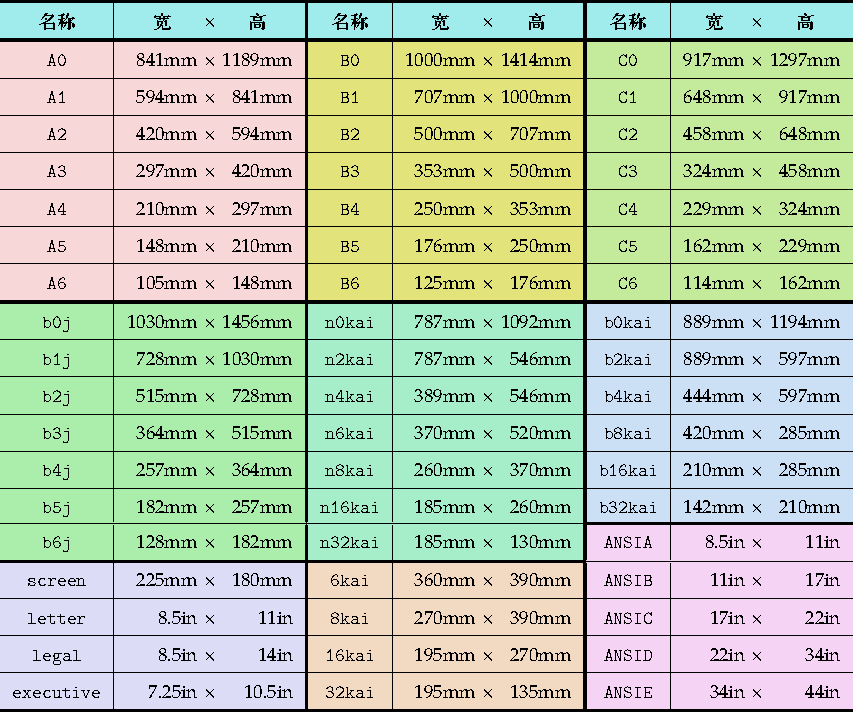
\includegraphics{cus-aux/tab-defined-papername}}
  \caption{预定义的纸张名}\label{tab:defined-papername}
\end{table}

\begin{keyval}[path=layout]{paperorientation,orientation,landscape,portrait,direction}
  \begin{syntax}
    paperorientation|orientation = <&landscape|portrait>
    landscape &&
    portrait  &&
    direction = <&bigwidth|bigheight|normal|inverse>
  \end{syntax}
设置纸张方向。使用 \opt{portrait} 时,纸张高度大于宽度。\opt{landscape} 则反之。

\opt{direction} 的 \opt{bigheight} 和 \opt{normal} 相当于 \opt{portrait},
\opt{bigwidth} 和 \opt{inverse} 相当于 \opt{landscape}。

使用 \opt{papername} 等选项时,将自动设置纸张方向,使得实际纸张宽高与所给一致。
\end{keyval}

\begin{keyval}[path=layout]{layout,layoutname,
  layoutwidth,layoutheight,layoutsize,
  layouthoffset,layoutvoffset,layoutoffset,centerlayout}
设置 \gpart{layout} 部分大小。

\opt{layout} 或 \opt{layoutname} 会根据纸张方向自动交换长宽,因此纸张方向必须先于它们设置。

\opt{centerlayout} 通过将 \opt{layoutfoffset} 和 \opt{layoutvoffset} 设置为合适的值,以将 
\gpart{layout} 部分置于纸张中心。

见 \pkgdoc{geometry}。
\end{keyval}

\subsection{主体尺寸}

此小节与 \pkg{geometry} 对应部分的用法和作用相同。

\begin{keyval}[path=layout]{hscale,vscale,scale}
  \begin{syntax}
    hscale = \marg{正实数} & 0.7
    vscale = \marg{正实数} & 0.7
    scale  = \{\meta{hscale},\meta{vscale}\} 或 \marg{正实数}
  \end{syntax}
设置 \gpart{total part} 部分的宽高与 纸张宽高的比率。
\end{keyval}

\begin{keyval}[path=layout]{totalwidth,width,totalheight,height,total}
  \begin{syntax}
    totalwidth |width  = \marg{长度}
    totalheight|height = \marg{长度}
    total              = \{\meta{totalwidth},\meta{totalheight}\} 或 \marg{长度}
  \end{syntax}
设置 \gpart{total part} 部分的宽高。
\end{keyval}

\begin{keyval}[path=layout]{textwidth,textheight,body,text}
  \begin{syntax}
    textwidth  = \marg{长度}
    textheight = \marg{长度}
    body       = \{\meta{textwidth},\meta{textheight}\}
    text       = \marg{长度}
  \end{syntax}
设置 \tn{textwidth}、\tn{textheight},即 \gpart{body} 部分的宽高。
\end{keyval}

\begin{keyval}[path=layout]{lines}
  \begin{syntax}
    lines = \marg{行数}
  \end{syntax}
根据 \meta{行数} 设置 \opt{textheight}。\meta{行数} 一般为正整数。
\end{keyval}

\begin{keyval}[path=layout]{includehead,includefoot,
  includeheadfoot,includehf}
  \begin{syntax}
    includehead = <&\TTF> & false 
    includefoot = <&\TTF> & false
    includeheadfoot|includehf = <&\TTF>
  \end{syntax}
控制是否将页眉(\tn{headheight}、\tn{headsep})、页脚(\tn{footskip})
计入 \gpart{total part} 部分中。
\end{keyval}

\begin{keyval}[path=layout]{includemarginpar,includemp}
  \begin{syntax}
    includemarginpar|includemp = <&\TTF> & false 
  \end{syntax}
控制是否将旁注(\tn{marginparwidth}、\tn{marginparsep})计入 \gpart{body} 部分中。
\end{keyval}

\begin{keyval}[path=layout]{includeall}
  \begin{syntax}
    includeall = <&\TTF> & false 
  \end{syntax}
设置 \opt{includeheadfoot} 及 \opt{includemarginpar}。
\end{keyval}

\begin{keyval}[path=layout]{ignorehead,ignorefoot,
  ignoreheadfoot,ignorehf}
  \begin{syntax}
    ignorehead = <&\TTF> & false 
    ignorefoot = <&\TTF> & false
    ignoreheadfoot|ignorehf = <&\TTF>
  \end{syntax}
在计算垂直方向的尺寸时,不考虑页眉、页脚。但不修改页眉页脚的尺寸。
\end{keyval}

\begin{keyval}[path=layout]{ignoremarginpar,ignoremp}
  \begin{syntax}
    ignoremarginpar|ignoremp = <&\TTF> & false 
  \end{syntax}
在计算水平方向的尺寸时,不考虑旁注的尺寸。但不修改旁注的尺寸。
\end{keyval}

\begin{keyval}[path=layout]{ignoreall}
  \begin{syntax}
    ignoreall = <&\TTF> & false 
  \end{syntax}
设置 \opt{ignoreheadfoot} 及 \opt{ignoremarginpar}。
\end{keyval}

\begin{keyval}[path=layout]{heightrounded}
  \begin{syntax}
    heightrounded = <&\TTF> & false
  \end{syntax}
如果设置为真,则将 \opt{textheight} 设置为不小于原 \opt{textheight} 且满足关系:
\[ n\times{}\text{\tn{baselineskip}}{}+{}\text{\tn{topskip}}\] 
的最小值。
\end{keyval}

% from geometry.dtx
\thisfloatsetup{margins=hangoutside,capposition=beside,
  capbesideposition={top,outside},floatwidth=\textwidth}
\begin{figure}[htb]
 \centering\small
 {\unitlength=.65pt
 \begin{picture}(460,525)(0,0)
 \put( 20,310){\framebox(120,170){}}
 \put( 20,507){\makebox(120,0)[bl]%
 {\textbf{(a)}~\opt{includeheadfoot}}}
 \put( 20,460){\line(1,0){120}}\put( 20,450){\line(1,0){120}}
 \put( 20,330){\line(1,0){120}}
 \put( 20,485){\makebox(120,0)[br]{\gpart{total body}}}
 \put( 20,335){\makebox(120,0)[bc]{\texttt{textwidth}}}
 \put(150,470){\makebox(0,0)[l]{\texttt{headheight}}}
 \put(150,450){\makebox(0,0)[l]{\texttt{headsep}}}
 \put(150,390){\makebox(0,0)[l]{\texttt{textheight}}}
 \put(150,320){\makebox(0,0)[l]{\texttt{footskip}}}
 \put( 10,460){\makebox(120,20)[bc]{\gpart{head}}}
 \put( 10,320){\makebox(120,140)[c]{\gpart{body}}}
 \put( 10,310){\makebox(120,10)[c]{\gpart{foot}}}
 \put(250,310){\framebox(120,170){}}
 \put(250,507){\makebox(120,0)[bl]%
 {\textbf{(b)}~\opt{includeall}}}
 \put(250,460){\line(1,0){95}}\put(250,450){\line(1,0){95}}
 \put(250,330){\line(1,0){95}}\put(345,330){\line(0,1){120}}
 \put(350,330){\line(0,1){120}}\put(350,450){\line(1,0){20}}
 \put(350,330){\line(1,0){20}}
 \put(250,485){\makebox(120,0)[br]{\gpart{total body}}}
 \put(250,460){\makebox(95,20)[bc]{\gpart{head}}}
 \put(250,320){\makebox(95,140)[c]{\gpart{body}}}
 \put(385,390){\makebox(95,0)[cl]%
 {\gpart{\shortstack[l]{marginal\\note}}}}
 \put(250,310){\makebox(95,10)[c]{\gpart{foot}}}
 \put(250,335){\makebox(95,0)[bc]{\texttt{textwidth}}}
 \multiput(360, 390)(4,0){6}{\line(1,0){2}}
 \multiput(348,333)(0,-4){12}{\line(0,1){2}}
 \multiput(360,333)(0,-4){8}{\line(0,1){2}}
 \put(355,292){\makebox(0,0)[bl]{\texttt{marginparwidth}}}
 \put(345,275){\makebox(0,0)[bl]{\texttt{marginparsep}}}
 \put( 20, 40){\framebox(120,170){}}
 \put( 20,237){\makebox(120,0)[bl]%
 {\textbf{(c)}~\opt{includefoot}}}
 \put( 20, 60){\line(1,0){120}}
 \put( 20,215){\makebox(120,0)[br]{\gpart{total body}}}
 \put(150,130){\makebox(0,0)[l]{\texttt{textheight}}}
 \put(150, 50){\makebox(0,0)[l]{\texttt{footskip}}}
 \put( 20, 50){\makebox(120,160)[c]{\gpart{body}}}
 \put( 20, 40){\makebox(120,10)[c]{\gpart{foot}}}
 \put( 20, 65){\makebox(120,10)[c]{\texttt{textwidth}}}
 \put(250, 40){\framebox(120,170){}}
 \put(250,237){\makebox(120,0)[bl]%
 {\textbf{(d)}~\opt{includefoot}, \opt{includemp}}}
 \put(250, 60){\line(1,0){95}}\put(350, 60){\line(1,0){20}}
 \put(250,215){\makebox(120,0)[br]{\gpart{total body}}}
 \put(250, 50){\makebox(95,160)[c]{\gpart{body}}}
 \put(385,130){\makebox(95,0)[cl]%
 {\gpart{\shortstack[l]{marginal\\note}}}}
 \put(250, 40){\makebox(95,10)[c]{\gpart{foot}}}
 \put(250, 65){\makebox(95,0)[bc]{\texttt{textwidth}}}
 \put(345, 60){\line(0,1){150}}\put(350, 60){\line(0,1){150}}
 \multiput(360, 130)(4,0){6}{\line(1,0){2}}
 \multiput(348, 63)(0,-4){12}{\line(0,1){2}}
 \multiput(360, 63)(0,-4){8}{\line(0,1){2}}
 \put(355,22){\makebox(0,0)[bl]{\texttt{marginparwidth}}}
 \put(345, 5){\makebox(0,0)[bl]{\texttt{marginparsep}}}
 \end{picture}}
 \captionsetup{labelsep=newline}
 \caption[不同模式下的 total part]{\small
 \ifLabelOdd{fig:geometry-modes}{\raggedright}{\raggedleft}%
  不同模式下的 \gpart{total body}。
  (a) \opt{includeheadfoot},(b) \opt{includeall},(c) \opt{includefoot}
  及 (d) \opt{includefoot},\opt{includemp}。
  如果 \opt{reversemarginpar} 设置为真,则交换 \gpart{marginal note} 与 \gpart{body}
  的位置。如果设置了 \opt{twoside},则依据奇偶页交换 \gpart{marginal note}。}
 \label{fig:geometry-modes}
\end{figure}

\begin{keyval}[path=layout]{hdivide,vdivide,divide}
  \begin{syntax}
    hdivide = \{\meta{left margin},\meta{width},\meta{right margin}\}
    vdivide = \{\meta{top margin},\meta{height},\meta{bottom margin}\}
    divide  = \{\meta{length_1},\meta{length_2},\meta{length_3}\}
  \end{syntax}
设置两个值,将另一个留空或 \verb|*|。
\end{keyval}


\subsection{边距}

\nofuncskip
\begin{keyval}[path=layout]{leftmargin,left,lmargin,inner,
  rightmargin,right,rmargin,outer,hmargin,horizontalmargin}
  \begin{syntax}
    lmargin|leftmargin |left |inner = \marg{内侧边距}
    rmargin|rightmargin|right|outer = \marg{外侧边距}
    hmargin|horizontalmargin  = \{\meta{inner},\meta{outer}\} 或 \marg{水平边距}
  \end{syntax}
设置内外侧边距。注意,不论是否使用 \opt{twoside},它们的含义都是相同的。
\end{keyval}

\begin{keyval}[path=layout]{topmargin,top,tmargin,bottommargin,bottom,bmargin,verticalmargin}
  \begin{syntax}
    tmargin|topmargin   |top    = \marg{顶部边距}
    bmargin|bottommargin|bottom = \marg{底部边距}
    vmargin|verticalmargin      = \{\meta{top},\meta{bottom}\} 或 \marg{垂直边距}
  \end{syntax}
设置上下边距。
\end{keyval}

\begin{keyval}[path=layout]{horizontalmarginratio,hmarginratio,
  verticalmarginratio,vmarginratio,marginratio}
  \begin{syntax}
    hmarginratio|horizontalmarginratio = \marg{inner ration}:\marg{outer ratio}
    vmarginratio|verticalmarginratio   = \marg{top ratio}:\marg{bottom ratio} & 2:3
    marginratio = \{\meta{hmargin ratio},\meta{vmargin ratio}\} 或 \marg{margin ratio}
  \end{syntax}
设置内外边距、上下边距的比率。

使用 \opt{oneside} 时 \opt{hmarginratio} 初始为 \texttt{1:1},
使用 \opt{twoside} 时 \opt{hmarginratio} 初始为 \texttt{2:3}。
\end{keyval}

\begin{keyval}[path=layout]{hcentering,vcentering,centering}
  \begin{syntax}
    hcentering = <&\TTF> 
    vcentering = <&\TTF> & false 
    centering  = <&\TTF>
  \end{syntax}
设置 \opt{hmarginratio}、\opt{vmarginratio} 为 \texttt{1:1}。
\end{keyval}

\begin{keyval}[path=layout]{twoside,asymmetric,reversemarginpar,reversemp}
  \begin{syntax}
    twoside &&
    asymmetric &&
    reversemarginpar|reversemp = <&\TTF> & false 
  \end{syntax}
设置左右边距根据奇偶页进行切换。\opt{asymmetric} 并不实际切换,而是修改长度,见 \pkgdoc{geometry}。
\end{keyval}

\begin{keyval}[path=layout]{bindingoffset}
  \begin{syntax}
    bindingoffset = \marg{长度}
  \end{syntax}
从内侧移除 \meta{长度}。
\end{keyval}

% from geometry.dtx
\thisfloatsetup{margins=hangoutside,capposition=beside,
  capbesideposition={top,outside},floatwidth=\textwidth}
\begin{figure}[htb]
 \centering\small
 {\unitlength=.65pt
 \begin{picture}(500,270)(0,0)
 \put(20,0){\framebox(170,230){}}
 \put(20,255){\makebox(80,20)[l]{\textbf{a)}~every page for oneside or}}
 \put(20,240){\makebox(80,20)[l]{\hspace{3ex}odd pages for twoside}}
 \put(110,225){\makebox(80,20)[r]{\gpart{paper}}}
 \put(55,37){\framebox(110,170)[tc]{\gpart{total body}}}
 \multiput(38,0)(0,7){33}{\line(0,1){4}}
 \put(38,100){\vector(1,0){17}}\put(55,100){\vector(-1,0){17}}
 \put(60,95){\makebox(80,10)[l]{\texttt{left}}}
 \put(60,80){\makebox(80,10)[l]{(\texttt{inner})}}
 \put(165,100){\vector(1,0){25}}\put(190,100){\vector(-1,0){25}}
 \put(195,95){\makebox(80,10)[l]{\texttt{right}}}
 \put(195,80){\makebox(80,10)[l]{(\texttt{outer})}}
 \put(20,16){\vector(1,0){18}}
 \put(45,10){\makebox(80,10)[bl]{\texttt{bindingoffset}}}
 \put(280,255){\makebox(80,20)[l]{\textbf{b)}~even (back) pages for twoside}}
 \put(280,0){\framebox(170,230){}}
 \put(370,225){\makebox(80,20)[r]{\gpart{paper}}}
 \put(305,37){\framebox(110,170)[tc]{\gpart{total body}}}
 \multiput(432,0)(0,7){33}{\line(0,1){4}}
 \put(280,100){\vector(1,0){25}}\put(305,100){\vector(-1,0){25}}
 \put(310,95){\makebox(80,10)[l]{\texttt{outer}}}
 \put(310,80){\makebox(80,10)[l]{(\texttt{right})}}
 \put(415,100){\vector(1,0){17}}\put(432,100){\vector(-1,0){17}}
 \put(373,95){\makebox(80,10)[l]{\texttt{inner}}}
 \put(373,80){\makebox(80,10)[l]{(\texttt{left})}}
 \put(450,16){\vector(-1,0){18}}
 \put(330,10){\makebox(80,10)[bl]{\texttt{bindingoffset}}}
 \end{picture}}
 \captionsetup{labelsep=newline}
 \caption[\texttt{bindingoffset} 选项]{%
  \ifLabelOdd{fig:bindingoffset}{\raggedright}{\raggedleft}\small
  The option \opt{bindingoffset} adds the specified length to the inner margin.
  Note that \opt{twoside} option swaps the horizontal margins and the
  marginal notes together with \opt{bindingoffset} on even pages (see
  \textbf{b}), but \opt{asymmetric} option suppresses the swap of the
  margins and marginal notes (but \opt{bindingoffset} is still swapped).}
 \label{fig:bindingoffset}
\end{figure}


\subsection{原有的变量}

本小节描述几个 \LaTeXe 原有的长度变量。

\begin{keyval}[path=layout]{footnotesep}
  \begin{syntax}
    footnotesep = \marg{弹性长度}
  \end{syntax}
设置 \tn{skip}\tn{footins},即正文底部与脚注顶部的距离。
\end{keyval}

\begin{keyval}[path=layout]{marginparwidth,marginpar,marginparsep,nomarginpar,nomp}
  \begin{syntax}
    marginparwidth|marginpar = \marg{长度}
    marginparsep = \marg{长度}
    nomarginpar|nomp &&
  \end{syntax}
设置旁注宽度及旁注与正文的距离。\opt{nomarginpar} 将它们设置为 \texttt{0pt}。
\end{keyval}

\begin{keyval}[path=layout]{columnsep,twocolumn,onecolumn}
  \begin{syntax}
    columnsep = \marg{长度}
    twocolumn &&
    onecolumn &&
  \end{syntax}
设置 \tn{columnsep},即两栏之间的距离。
\end{keyval}

\begin{keyval}[path=layout]{hoffset,voffset,offset}
  \begin{syntax}
    hoffset = \marg{长度}
    voffset = \marg{长度}
    offset  = \{\meta{hoffset},\meta{voffset}\} 或 \marg{长度}
  \end{syntax}
设置 \tn{hoffset}、\tn{voffset}。
\end{keyval}


\subsection{页眉页脚}\label{sec:geometry-headfoot}

\nofuncskip 
\begin{keyval}[path=layout]{headheight,head,headsep}
  \begin{syntax}
    head|headheight = \marg{长度}
    headsep = \marg{长度}
    nohead
  \end{syntax}
\opt{headheight} 设置 \tn{headheight},即页眉的高度。

\opt{headsep} 设置 \tn{headsep},即页眉与正文之间的距离。

\opt{nohead} 将它们设置为 \texttt{0pt}。
\end{keyval}

\begin{keyval}[path=layout]{footskip,foot,nofoot}
  \begin{syntax}
    footskip|foot = \marg{弹性长度}
  \end{syntax}
设置 \tn{footskip},即正文最后一行的基线与页脚基线的距离。

\opt{nofoot} 将它设置为 \texttt{0pt}。
\end{keyval}

\begin{keyval}[path=layout]{noheadfoot,nohf}
  \begin{syntax}
    noheadfoot|nohf &&
  \end{syntax}
同时设置 \opt{nohead} 和 \opt{nofoot}
\end{keyval}

\begin{keyval}[path=layout]{headoffset,footoffset,hfoffset}
  \begin{syntax}
    headoffset = \marg{长度} & 0pt 
    headoffset = \oarg{位置} \marg{长度}
  \end{syntax}
设置页眉页脚偏移量。

\meta{位置} 为 \texttt{O}、\texttt{E} 与 \texttt{L}、\texttt{C}、\texttt{R} 的组合。
这五个值分别代表奇偶、左中右。不区分大小写。

若 \meta{长度} 为正值,则相较于 \opt{textwidth} 伸长 \meta{长度}。否则,缩短 \meta{长度}。

此选项在直排文档中可能无效。
\end{keyval}

\subsection{杂项}

本小节列出其它几个选项。未列出的选项请参考 \pkgdoc{geometry}。

% \nofuncskip
\begin{keyval}[path=layout]{showframe,showcrop,showmarking,marking}
  \begin{syntax}
    showframe = <&\TTF> & false 
    showcrop  = <&\TTF> & false 
    showmarking|marking = <&\TTF> & false 
  \end{syntax}
\opt{showframe} 显示各部分的外框。\opt{showcrop} 在 \gpart{layout} 四角显示裁剪标记。
\opt{marking} 在各部分着以彩色背景。
\end{keyval}

\begin{keyval}[path=layout]{preset,name}
  \begin{syntax}
    preset|name = \marg{preset name}
  \end{syntax}
使用预设值 \meta{preset name}。
\end{keyval}

% \begin{keyval}[path=layout]{verbose}
%   \begin{syntax}
%     verbose = <&\TTF> & false 
%   \end{syntax}
% 将各变量的结果显示在终端中。设置为 \opt{false} 时,仍将其写入日志文件中。

% 仅可用于导言区。
% \end{keyval}

% \begin{keyval}[path=layout]{pass}
%   \begin{syntax}
%     pass &&
%   \end{syntax}
% 仅可用于导言区。
% \end{keyval}


\subsection{设置页眉页脚}\label{sec:pagestyle}

本小节设置页眉页脚内容的接口。关于设置页眉页脚位置和高度的接口,见\cref{sec:geometry-headfoot}。

本节所述内容可能在直排文档中不可用。

本节所述的功能主要通过 \pkg{fancyhdr} 实现。

\begin{function}{\usepagestyle}
  \begin{syntax}
    \verb|\usepagestyle| \marg{pagestyle}
  \end{syntax}
使用页眉页脚的样式 \meta{pagestyle}。

有一个预定义的样式 \texttt{totalempty},它将页眉页脚设置为空,并将页眉页脚横线的厚度设为 \texttt{0pt}。
\end{function}

\begin{function}{\setpagestyle}
  \begin{syntax}
    \verb|\setpagestyle|   \marg{pagestyle} \marg{code}
    \verb|\setpagestyle|   \marg{pagestyle_1} \oarg{pagestyle_2} \marg{code}
    \verb|\setpagestyle| * \marg{pagestyle_1} \oarg{pagestyle_2} \marg{code}
  \end{syntax}
设置样式 \marg{pagestyle},或基于样式 \meta{pagestyle_2} 设置 \meta{pagestyle_1}。

带 \verb|*| 的,仅设置而不使用。不带 \verb|*| 的,还会立刻使用该样式。
\end{function}

\begin{function}{\sethead,\setfoot,\setheadfoot,
  \setlefthead,\setcenterhead,\setrighthead,
  \setleftfoot,\setcenterfoot,\setrightfoot}
  \begin{syntax}
    \verb|\sethead|         \,\marg{code}
    \verb|\sethead| \oarg{位置} \marg{code}
    \verb|\setcenterhead|           \,\marg{奇偶页}
    \verb|\setcenterhead| \oarg{偶数页} \marg{奇数页}
  \end{syntax}
设置页眉页脚的内容。

\meta{位置} 为 \texttt{O}、\texttt{E}, \texttt{L}、\texttt{C}、\texttt{R},\texttt{H}、\texttt{F} 此三类的组合。
这七个个值分别代表奇偶、左中右、页眉页脚。不区分大小写。

如某一类未给出,则视为该类的全部值都给出。但 \cs{sethead}、\cs{setfoot} 分别为 \texttt{H}、\texttt{F}。

例如,在 \cs{sethead} 中,\verb|L| 代表 \verb|OLF,ELF|。

它们可以直接用在导言区和正文中,将修改本页及其后页面的页眉页脚。但最好用于 
\cs{setpagestyle} 命令中,统一设置页眉页脚。
\end{function}

\begin{function}{\setheadrulewidth,\setfootrulewidth}
  \begin{syntax}
    \verb|\setheadrulewidth| \marg{长度表达式}
  \end{syntax}
设置页眉、页脚横线的厚度。

(即宏 \tn{headrulewidth}、\tn{footrulewidth} 的值。)
\end{function}

\begin{function}{\setheadruleskip,\setfootruleskip}
  \begin{syntax}
    \verb|\setheadruleskip| \marg{skip expr}
  \end{syntax}
设置页眉、页脚横线与页眉、页脚文字的距离。

(即宏 \tn{headruleskip}、\tn{footruleskip} 的值。)
\end{function}

\begin{function}{\setheadrule,\setfootrule}
  \begin{syntax}
    \verb|\setheadrule| \marg{code}
  \end{syntax}
设置页眉、页脚的横线。页眉的横线的总高度最好为 0。
\end{function}

\begin{function}{\setheadinit,\setfootinit,\setheadfootinit}
  \begin{syntax}
    \verb|\setheadinit| \marg{code}
  \end{syntax}
在输出页眉页脚前要执行的 \meta{code}。
\end{function}

\begin{function}{\fancycenter}
  \begin{syntax}
    \verb|\fancycenter| \marg{left} \marg{center} \marg{right}
    \verb|\fancycenter| \oarg{distance} \oarg{stretch} \marg{left} \marg{center} \marg{right}
  \end{syntax}
它创建一个盒子,使得 \meta{center} 位于当前行(或盒子)的中心。可以用于正文中。

\meta{center} 的中心与 \meta{left}、\meta{right} 的中心的距离可能并不一致。
\end{function}

\begin{xample}
\fancycenter{L}{CCCC}{RRRRRRRRRRRRRRRR}
\stopxamplecode
\xampleprint
\end{xample}

\begin{function}[EXP]{\iftopfloat,\ifbotfloat,\iffloatpage,\iffootnote}
  \begin{syntax}
    \verb|\iftopfloat| \marg{true} \marg{false}
  \end{syntax}
检测当前页是否顶部、底部有浮动体,或当前页是否是浮动体页,或当前页是否有脚注。
\end{function}


\section{盒子和填充,\cusmodule{box}模块}

\cusmodule{box} 用于提供盒子构造、内容填充等内容。


\subsection{Framed}

\cusmodule{box} 模块定义了一个简易的可跨页的盒子环境 \env{Framed},相较于 
\pkg{tcolorbox} 宏包提供的环境来说,使用此环境的速度更快。它也可配合 \pkg{tcolorbox}
宏包使用。

\begin{function}[type=environment]{Framed}
  \begin{syntax}
    \verb|\begin{Framed}| \oarg{frame key-val}
    ~~... 
    \verb|\end{Framed}|
  \end{syntax}
创建一个可跨页的盒子。若在另一个盒子内则不可跨页。
\end{function}

\begin{keyval}[path=frame]{outer-sep}
  \begin{syntax}
    outer-sep = \marg{skip expr} & 8pt plus 8pt minus 6pt 
  \end{syntax}
设置盒子与上下文的间距。
\end{keyval}

\begin{keyval}[path=frame]{sep}
  \begin{syntax}
    sep = \marg{长度表达式} & \V{3\fboxsep}
  \end{syntax}
设置变量 \tn{cusframesep},即盒子外框与内容的间距。
\end{keyval}

\begin{keyval}[path=frame]{rule-width}
  \begin{syntax}
    rule-width = \marg{长度表达式} & \V\fboxrule
  \end{syntax}
设置变量 \tn{cusframerule},即盒子外框的厚度。
\end{keyval}

\begin{keyval}[path=frame]{frame,frame*,
  first,first*,middle,middle*,last,last*,
  whole,whole*}
  \begin{syntax}
    frame  = \marg{code}
    frame* = \marg{code width 1 parameter}
  \end{syntax}
\opt{frame} 设置盒子外框。

\opt{first},\opt{middle},\opt{last} 设置分页盒子的前、中、后三部分的外框。

\opt{whole} 设置未分页盒子的外框。

\meta{code} 其后可接一个参数,这个参数为分页后的盒子。
\meta{code with 1 parameter} 显式给出变量 \verb|#1|。
\end{keyval}

\begin{keyval}[path=frame]{init}
  \begin{syntax}
    init = \marg{code}
  \end{syntax}
盒子中执行的初始化代码。
\end{keyval}

\begin{keyval}[path=frame]{width,ratio}
  \begin{syntax}
    width = \marg{长度表达式} & \V\textwidth
    ratio = \marg{数值表达式} & 1
  \end{syntax}
\opt{ratio} 设置盒子内容(含边框)占 \opt{width} 的比率。
\end{keyval}

\begin{keyval}[path=frame]{align,
  left,center,right,inner,outer}
  % absinner,absouter,inner*,outer*,
  \begin{syntax}
    align = <&left|center|right|inner|outer> & center 
  \end{syntax}
设置水平对齐方式。当 $ 0 <{} \text{\meta{ratio}} {}< 1 $ 时才有效。
\end{keyval}

\begin{xample}
\begin{Framed}[ratio=.8,center,
  rule-width=2pt,
  frame={\setlength{\fboxsep}{\cusframesep}%
          \setlength{\fboxrule}{\cusframerule}%
          \fcolorbox{purple}{cyan!50}}]
\zhlipsum[9][name=zhufu]
\end{Framed}
\stopxamplecode
\xampleprint 
\vskip 1pt 
\end{xample}

\begin{keyval}[path=frame]{ignore-warnings}
  \begin{syntax}
    ignore-warnings &&
  \end{syntax}
忽略部分警告。
\end{keyval}


\subsection{Filler}

“filler”是用以填充空间的那部分内容。如 \LaTeXe 的 \tn{hrulefill} 是用水平直线填充,
\tn{dotfill} 是用句点填充,\tn{hspace} 是用空白填充。

\cusmodule{box} 提供了几个创建 filler 的命令。

\begin{function}{\dashfiller}
  \begin{syntax}
    \verb|\dashfiller|
    \verb|\dashfiller| \marg{filler width}
    \verb|\dashfiller| \oarg{raise}\oarg{sep width}\oarg{rule width}
    \verb|\dashfiller| \oarg{raise} \marg{filler width}\oarg{sep width}\oarg{rule width}
  \end{syntax}
使用虚线填充,虚线宽和虚线间的距离近似为 \meta{sep width},使得虚线充满 \meta{filler width}。

\begin{itemize}[nosep]
  \item \meta{filler width} 为总宽度,默认值为 \tn{linewidth}。
  \item \meta{raise} 为虚线升高的高度,默认为 \texttt{0pt}。
  \item \meta{sep width} 为虚线宽和虚线间的距离,默认为 \texttt{1ex}。
  \item \meta{rule width} 为虚线的厚度,默认为 \texttt{0.4pt}。
\end{itemize}
\end{function}

\begin{xample}
\noindent\llap{|}\dashfiller \par % 总长为 \linewidth 
\noindent\llap{|}\dashfiller [.5ex] \par % 升高 .5ex
% 升高 .5ex,宽 3pt,注意第二个可选参数前不能有空格
\noindent\llap{|}\dashfiller [.5ex][3pt] \par 
\stopxamplecode
\xampleprint 
\end{xample}

\begin{function}{\filler}
  \begin{syntax}
    \verb|\filler| \oarg{filler key-val}
  \end{syntax}
使用给定内容填充。
\end{function}

\begin{keyval}[path=filler]{size,size*}
  \begin{syntax}
    size  = \marg{skip expr}
    size* = \marg{长度}
  \end{syntax}
设置填充的长度。\opt{size*} 填充的长度是弹性的。

注意在行间数学模式中(\env{equation}、\env{align} 等环境)弹性的那部分长度无效。
\end{keyval}

\begin{keyval}[path=filler]{space,hspace,hspace*,vspace,vspace*,not-space}
  \begin{syntax}
    space   = \marg{code}
    hspace  = \marg{skip expr}
    hspace* = \marg{skip expr}
    vspace  = \marg{skip expr}
    vspace* = \marg{skip expr}
    not-space &&
  \end{syntax}
使用空白填充。使用它后,其它选项无效。

\meta{code} 是填充的内容,如 \verb|\hspace{1cm}|,\verb|\vspace*{1cm}|。

\opt{hspace} 相当于设置 \verb|space=\hspace|\marg{skip expr}。

\opt{hspace*} 相当于设置 \verb|space=\hspace*|\marg{skip expr}。

\opt{vspace} 相当于设置 \verb|space=\vspace|\marg{skip expr}。

\opt{vspace*} 相当于设置 \verb|space=\vspace*|\marg{skip expr}。

由于用 space 填充的优先级最高,若设置使用 space 填充后,要使用其它类型来填充,需使用
\opt{not-space} 或将 \opt{space} 设置为空。若后续仍设置了 \opt{space},则仍会使用 space 填充。
\end{keyval}

\begin{xample}
左 \fbox{\strut \filler [hspace=5cm]} 右间隔约 5cm。

左 \filler[space] 右拉开。

左 \filler[space] 中 \filler[space] 右拉开。
\stopxamplecode
\xampleprint
\end{xample}

\begin{keyval}[path=filler]{color}
  \begin{syntax}
    color = <{color expr}>
  \end{syntax}
设置颜色 \key[module=color name]{cusfiller},即填充的颜色。
\end{keyval}

\begin{keyval}[path=filler]{content,box,box*,clear-box}
  \begin{syntax}
    content = <{content}>
    box     = <{content}>
    box*    = <{长度表达式}> <{content}>
    clear-content &&
    clear-box &&
    not-content &&
  \end{syntax}
使用长 \meta{长度表达式} 的 \meta{content} 填充。

\opt{content} 和 \opt{box} 选项基本一致,只是 \opt{content} 会自动设置颜色,而
\opt{box} 则需使用 \tn{color} 或 \cs{color_select:n} 来设置颜色。

使用 \opt{content} 将使用 \meta{content} 的自然宽度,而 \opt{box*} 则使用指定的宽度。

当设置了 \opt{box} 或 \opt{box*} 后,\opt{content} 无效,除非使用 \opt{clear-box} 清除 box。
\end{keyval}

\begin{keyval}[path=filler]{dash,sep,rule,raise,full,is-dash}
  \begin{syntax}
    dash|sep = \marg{dash length} & 0pt 
    rule     = \marg{rule width} & 0.4pt 
    raise    = \marg{raise height} & 0pt 
    full     = <&\TTF> & false 
    is-dash &&
  \end{syntax}
使用虚线填充。

虚线宽和虚线间距为 \meta{dash length},厚度为 \meta{rule width},升高 \meta{raise height}。

若 \meta{dash length} 为 \texttt{0pt},则使用实线填充。

如果设置 \opt{full} 为真,则相当于 \cs{dashfiller}。
\end{keyval}

\begin{keyval}[path=filler]{solid,dashed,dotted,cdotted}
  \begin{syntax}
    solid &&
    dashed  = \marg{长度}
    dotted  = \marg{间距}
    cdotted = \marg{间距}
  \end{syntax}
使用实线、虚线、句点或 \tn{cdot} 填充。
\end{keyval}

\begin{xample}
\def\BL{\noindent\llap{|}}%
\BL \filler[color=red, solid, rule=2pt] \par
\BL \filler[color=red, dashed, rule=0.5ex] \par 
\BL \filler[color=red, dashed, rule=0.5ex, full] \par 
\BL \filler[color=red, dotted] \par 
\BL \filler[color=red, cdotted] \par 
\BL \filler[color=red, cdotted=1cm, align] \par % 每个点都是对齐的
\BL \filler[color=red, cdotted=1cm, center] \par % 每个点的间距都是 1cm
\BL \filler[color=red, cdotted=1cm, spread] % 每个点的间距都相等,可能超过1cm
\stopxamplecode
\xampleprint
\end{xample}

\begin{keyval}[path=filler]{type,align,center,spread}
  \begin{syntax}
    type  = <&align|center|spread> & align 
    align &&
    center &&
    spread &&
  \end{syntax}
构造填充的方式。

\begin{itemize}[nosep]
  \item \opt{align}:每个同种 filler 都是无限长的对齐的填充中的一部分,因此,它们处处都是对齐的;
  \item \opt{center}:把用以填充的盒子紧挨着排列,两头留下相等的空白;
  \item \opt{spread}:把多余的空白均匀地分布在盒子中间及两侧。
\end{itemize}
\end{keyval}

\begin{texnote}
实际这三种方式分别对应 \tn{leaders}、\tn{cleaders}、\tn{xleaders}。
\end{texnote}

\begin{function}{\atleastfiller}
  \begin{syntax}
    \verb|\atleastfiller| \marg{dim expr}
    \verb|\atleastfiller| \oarg{filler key-val} \marg{dim expr}
  \end{syntax}
填充的长度至少为 \meta{dim epxr},太短的将自动断行。
\end{function}

\begin{xample}
我能吞下玻璃而不伤身体,I can eat glass, it dosen't hurt me.%
\atleastfiller[cdotted=1em]{5cm}断行。

我能吞下玻璃而不伤身体。\atleastfiller[cdotted=1em]{5cm}不断。
\stopxamplecode
\xampleprint 
\end{xample}

\begin{function}{\breakablefiller}
  \begin{syntax}
    \verb|\breakablefiller|
    \verb|\breakablefiller| \oarg{filler key-val}
  \end{syntax}
可自动断行的 filler。
\end{function}

\begin{xample}
\framebox[3cm]{可断} \breakablefiller[cdotted=1em] \framebox[3cm]{模式。}

\framebox[7cm]{可断} \breakablefiller[cdotted=1em] \framebox[7cm]{模式。}
\stopxamplecode
\xampleprint
\end{xample}

下例展示了制作多行填充的例子。
\begin{xample}
\newcommand\filllines[4][]{{% filler key-val, before, lines, after
  #2\filler[#1]%
  \Replicate{#3-1}{\break \rule{0pt}{0.7\baselineskip}\filler[#1]}%
  #4\par}}

我能吞下玻璃而不伤身体,I can eat glass, it dosen't hurt me.
\filllines{\linespread{2}\selectfont}{3}{。\hspace*{1em}}

我能吞下玻璃而不伤身体,I can eat glass, it dosen't hurt me.
\filllines[color=red,dotted]{\linespread{2}\selectfont}{3}{。\hspace*{1em}}

% 整行
\filllines [raise=-.5ex]{\linespread{2}\selectfont \noindent\strut}{3}{ 整行。\hspace*{1em}}
\stopxamplecode
\xampleprint  
\end{xample}


\subsection{多栏文字}\label{sec:multicol}

\CusTeX 中排版多栏文字有两种方式,本节描述其中一种,使用 \pkg{multicol} 宏包实现。另一种方式见\cref{sec:lib-box}。

在 \pkg{multicol} 中,可以使用 
\begin{xample}
\begin{multicols}{col}
  ... 
\end{multicols}
\stopxamplecode 
\xamplecode \medskip 
\end{xample}
来排版多栏文字。本模块对其进行了简单的封装,使得可以通过键值方式来设置相关变量。

关于每个内部变量的详细用法,可以参考 \pkgdoc{multicol}。

\begin{function}{\startmulticolumns,\stopmulticolumns}
  \begin{syntax}
    \verb|\startmulticolumns| \oarg{multicolumns key-val}
    ~~<content>
    \verb|\stopmulticolumns|
  \end{syntax}
将 \meta{content} 以多栏排版。
\end{function}

\begin{keyval}[path=multicolumns]{columns,cols}
  \begin{syntax}
    columns|cols = \marg{整数表达式} & 2
  \end{syntax}
设置多栏数。也可不必写出键名,只写数字。

可用的栏数为 1--20,如果 \keyref[multicolumns]{adj} 为
\opt{true},则可用的栏数为 1--10。
\end{keyval}

\begin{keyval}[path=multicolumns]{outer-sep}
  \begin{syntax}
    outer-sep = \marg{skip expr} & 12.0pt plus 4.0pt minus 3.0pt
  \end{syntax}
设置 \tn{multicolsep},即多栏文字与上下文的间距。
\end{keyval}

\begin{keyval}[path=multicolumns]{column-sep,sep}
  \begin{syntax}
    column-sep|sep = \marg{length} & 10pt 
  \end{syntax}
设置 \tn{columnsep},即多栏文字两栏的间隙。
\end{keyval}

\begin{keyval}[path=multicolumns]{first-minimal,last-minimal}
  \begin{syntax}
    first-minimal = \marg{pre length} & 50pt 
    last-minimal  = \marg{post length} & 20pt 
  \end{syntax}
如果多栏开始的那一页不足 \meta{pre length},则多栏将在新的一页开始。

如果多栏结束的那一页不足 \meta{post length},则多栏将在新的一页结束。

\opt{first-minimal} 设置 \tn{premulticols},
\opt{last-minimal} 设置 \tn{postmulticols}。
\end{keyval}

\begin{keyval}[path=multicolumns]{heading}
  \begin{syntax}
    heading = \marg{content}
  \end{syntax}
设置在多栏文字之前的横跨所有栏的文字。可以使用 \tn{section} 等。它与其后的多栏文字保持在同一页。
\end{keyval}

\begin{keyval}[path=multicolumns]{rule-width,rule-color}
  \begin{syntax}
    rule-width = \marg{length} & 0pt 
    rule-color = \marg{color}
    rule-color = \oarg{color mode} \marg{color}
  \end{syntax}
设置 \tn{columnseprule}、\tn{columnseprulecolor},即多栏间竖线的宽度和颜色。
\end{keyval}

\begin{keyval}[path=multicolumns]{flush,aligned,ragged,not-aligned}
  \begin{syntax}
    flush |aligned &&
    ragged|not-aligned &&
  \end{syntax}
控制多栏文字的尾部是否对齐。分别设使用 \tn{flushcolumns} 和 \tn{raggedcolumns}。

初始为 \opt{aligned},将使各栏头部和尾部的基线尽量对齐。
\end{keyval}

\begin{keyval}[path=multicolumns]{balanced,not-balanced}
  \begin{syntax}
    balanced = <&\TTF> & true 
    not-balanced &&
  \end{syntax}
在末页文字的处理上,有两种方式,一种为文字尽量往上排,而将下方留空,这也是默认的方式;
另一种为文字尽量往左排(右排),而将右边(左边)留空,也就是将空白留在末尾的几栏上。
前者为 \opt{balanced},后者为 \opt{not-balanced}。
\end{keyval}

\begin{keyval}[path=multicolumns]{columns*,cols*}
  \begin{syntax}
    columns*|cols* = \marg{栏数}
  \end{syntax}
它在设置栏数的同时还设置 \opt{not-balanced}。

注意 \opt{columns} 并未决定使用 \opt{balanced} 还是 \opt{not-balanced}。
\end{keyval}

\begin{keyval}[path=multicolumns]{swap-column,enable-swap-column,disable-swap-column}
  \begin{syntax}
    swap-column = <&\TTF> & false 
    enable-swap-column &&
    disable-swap-column &&
  \end{syntax}
控制是否在使用了 \opt{twoside} 文档类选项时,偶数页逆序输出各栏。

\opt{enable-swap-column} 用于启用此功能,\opt{disable-swap-column} 用于禁用此功能。
\end{keyval}

\begin{keyval}[path=multicolumns]{framed,framed-options,framed-options+}
  \begin{syntax}
    framed = <&fbox|...>
    framed-options = \marg{options}
  \end{syntax}
控制多栏文字整体用哪种盒子框住,多栏文字仍然可以分页。
\opt{framed-options} 为可能的选项。

默认仅提供 \opt{fbox} 这个可选值,表示用 \tn{fbox} 框住。其它库可能提供额外的值。如 
\cusmodule{tcb} 库提供 \opt{tcbox} 值(\cref{sec:multicolumns/framed=tcbox}),
\cusmodule{box} 库提供 \opt{lfbox} 值(\cref{sec:multicolumns/framed=lfbox})。

使用此选项时,最好把 \keyref[multicolumns]{overflow} 设置为 \texttt{0pt},否则可能无法正常分页。
\end{keyval}

\begin{keyval}[path=multicolumns]{adj,adj-inner,adj-outer}
  \begin{syntax}
    adj = <&\TTF> & false 
    adj-inner = \marg{内侧长度}
    adj-outer = \marg{外侧长度}
  \end{syntax}
多栏文字还可以通过调整边距来调整总的文字宽度。\opt{adj} 用于启用此功能。

\meta{内侧长度} 和 \meta{外侧长度} 分别调整文字的内侧和外侧边距。正值表示向文字内调整
(总的文字宽度减少),负值表示向文字外调(总的文字宽度增加)。
它们自动设置 \opt{adj} 为 \opt{true}。
\end{keyval}

\sdanger

\begin{keyval}[path=multicolumns]{addto-baselineskip}
  \begin{syntax}
    addto-baselineskip = \marg{length}
  \end{syntax}
设置 \tn{multicolbaselineskip}。% 将 \meta{length} 加到 \tn{baselineskip} 上。
\end{keyval}

\begin{keyval}[path=multicolumns]{tolerance,pretolerance}
  \begin{syntax}
    tolerance    = \marg{int expr} & 9999
    pretolerance = \marg{int expr}
  \end{syntax}
设置 \tn{multicoltolerance}、\tn{multicolpretolerance}。
\end{keyval}

\begin{keyval}[path=multicolumns]{collectmore,minrows,unbalance,column-badness,final-column-badness}
  \begin{syntax}
    collectmore = \marg{int expr}
  \end{syntax}
设置 \texttt{collectmore},\texttt{minrows},\texttt{unbalance},
\texttt{columnbadness},\texttt{finalcolumnbadness} 计数器。
\end{keyval}

\begin{keyval}[path=multicolumns]{top-fuzz,bottom-fuzz}
  \begin{syntax}
    top-fuzz    = \marg{dim expr} & 0pt 
    bottom-fuzz = \marg{dim expr} & 2pt 
  \end{syntax}
设置 \tn{multicolovershoot}、\tn{multicolundershoot}。
\end{keyval}

\begin{keyval}[path=multicolumns]{v-fuzz,h-fuzz}
  \begin{syntax}
    v-fuzz = \marg{length}
  \end{syntax}
\opt{v-fuzz} 设置 \opt{top-fuzz} 和 \opt{bottom-fuzz}。\opt{h-fuzz} 设置 \tn{hfuzz}。
\end{keyval}

\begin{keyval}[path=multicolumns]{overflow}
  \begin{syntax}
    overflow = \marg{dim expr} & 12pt 
  \end{syntax}
设置 \tn{maxbalancingoverflow}。
\end{keyval}

\begin{keyval}[path=multicolumns]{left-to-right,LR,right-to-left,RL}
  \begin{syntax}
    left-to-right|LR &&
    right-to-left|RL &&
  \end{syntax}
使用 \tn{LRmulticolcolumns} 或 \tn{RLmulticolcolumns}。默认为 \opt{left-to-right}。
\end{keyval}

\subsection{旋转的盒子}

\CusTeX 封装了 \pkg{rotating} 宏包,提供了旋转的盒子。

\begin{function}{\startrotate,\stoprotate,\Rotate}
  \begin{syntax}
    \verb|\startrotate| \oarg{rotate key-val}
    ~~\meta{content}
    \verb|\stoprotate|
    \endgraf \medskip 
    \verb|\Rotate| \oarg{rotate key-val} \marg{content}
  \end{syntax}
将 \meta{content} 旋转显示。
\end{function}

旋转的盒子有两种方式,一种为保留旋转后的盒子的大小,另一种设置旋转后的盒子大小为 0。

\begin{keyval}[path=rotate]{turn,nospaceturn,rotate,sideways}
  \begin{syntax}
    turn = \marg{number}
    rotate|nospaceturn = \marg{number}
    sideways &&
  \end{syntax}
将盒子旋转 \meta{number} 度。一般是逆时针旋转。

\opt{turn} 使用第一种方式,\opt{rotate} 使用第二种方式。\opt{sideways} 相当于 \verb|turn=90|。

\verb|\startrotate ... \stoprotate| 默认使用 \opt{turn},\verb|\Rotate| 默认使用
\opt{rotate}。
\end{keyval}

\begin{keyval}[path=rotate]{float,float*,figure,figure*,table,table*}
  \begin{syntax}
    float  = \marg{float type}
    float* = \marg{float type}
    figure &&
    figure* &&
  \end{syntax}
将 \meta{content} 看作在浮动环境 \meta{float type} 内,并将其旋转 90 度。旋转后的内容占据一整个页面。

带 \verb|*| 类似于带 \verb|*| 的浮动环境。

也可不写出 \opt{float} 或 \opt{float*} 键名,直接写 \meta{float type} 或 
\meta{float type}\verb|*|。
\end{keyval}


\section{背景,\cusmodule{bgfg}模块}

\cusmodule{bgfg} 是对 \texttt{shipout} 钩子的简单封装。

关于“钩子”机制,\cref{sec:lthooks}对其作了简单的介绍,更详细的用法请参考:\file{lthooks.pdf}。

本手册前几页的水印使用如下代码实现:
\begin{xample}
% 将盒子的内容添加到背景上
\background + [./watermark]{%
  \rotatebox{45}{\color{gray!30}\fontsize{100}{0}%
    \sffamily \CusTeX}}

% 使用如下代码即可删除此背景
\removebackground[./watermark]
\stopxamplecode
\xamplecode
\medskip 
\end{xample}

\begin{function}{\foreground,\background}
  \begin{syntax}
    \verb|\foreground|   \marg{content}
    \verb|\foreground| + \marg{content}
    \verb|\foreground| \parg{位置} \marg{content}
    \verb|\foreground| \oarg{hook label} \marg{content}
    \verb|\foreground| + \parg{位置} \oarg{hook label} \marg{content}
  \end{syntax}
将 \meta{content} 放置在前景或背景中。

\begin{itemize}[nosep]
  \item \meta{content} 为要放置的内容,该内容将完整地嵌于页面内;
  \item \meta{位置} 是 \meta{content} 要放置的位置,为两个字符,前一个为水平位置;后一个为垂直位置。水平位置包括:左(\texttt{l})、右(\texttt{r})、内侧(\texttt{i})、外侧(\texttt{o});垂直位置包括:顶部(\texttt{t})、底部(\texttt{b});它们的组合也就是 \gpart{layout} 的四个角。此外还有一个 \texttt{cm},它表示 \gpart{layout} 的正中心,这也是默认值;
  \item \meta{hook label} 为 hook 的 label;此参数与 \meta{位置} 的先后位置可交换;\\ 
  \cs{foreground} 默认为 \texttt{./fg},\cs{background} 默认为 \texttt{./bg};\\
  关于 hook label 的作用,请参考\cref{sec:lthooks}或 \file{lthooks.pdf};
  \item 默认情况下 \meta{content} 仅添加到当前页,使用 \texttt{+} 可将 \meta{content} 添加到往后各页。
\end{itemize}
\end{function}

除了上述两个命令外,还提供了两个设置背景图片的命令。

\begin{function}{\foregroundpicture,\backgroundpicture}
  \begin{syntax}
    \verb|\foregroundpicture|     \marg{图片}
    \verb|\foregroundpicture| +   \marg{图片}
    \verb|\foregroundpicture|   * \marg{图片}
    \verb|\foregroundpicture| + * \marg{图片}
    \verb|\foregroundpicture| + * \parg{位置} \oarg{hook label} \marg{图片}
  \end{syntax}
将 \meta{图片} 添加到前景或背景中。

\texttt{+}、\meta{位置}、\meta{hook label} 的用法如前所述。

不带 \verb|*| 的图片被伸缩到与 \gpart{layout} 同宽高。而带星号的则仅缩放宽度,保持纵横比例不变。
\end{function}

也可直接使用 \cs{background} 放置背景图片。
\begin{xample}
\background(ob){
\includegraphics[width=\marginparwidth]{ctanlion.pdf}}
\stopxamplecode
\xampleprint
如本页底部图片所示。
\end{xample}

% \begin{xample}
% \backgroundpicture*{ctanlion.pdf}
% \stopxamplecode
% \xampleprint
% 效果如本页所示。
% \end{xample}

\begin{function}{\removeforeground,\removebackground}
  \begin{syntax}
    \verb|\removeforeground|
    \verb|\removeforeground| \oarg{hook label}
  \end{syntax}
移除前景或背景。
\end{function}


\section{索引,\cusmodule{index}模块}

\CusTeX 提供了添加多个索引的方法。并且能够自动编译索引文件。

目前暂未提供 \pkg{splitidx} 宏包的功能,也不与其兼容。

应该与 \pkg{glossaries} 宏包兼容。

\begin{function}{\newindextype,\setupindex}
  \begin{syntax}
    \verb|\newindextype| \oarg{index keys} \marg{index type}
    \verb|\setupindex|   \oarg{index type list} \marg{index keys}
  \end{syntax}
\cs{newindextype} 创建一个新的索引 \meta{index type}。
\cs{setupindex} 配置 \meta{index type list}。
\meta{index type} 可以使用 \tn{empty} 作为名称,此时它的名称为空。
\end{function}

\begin{function}{\makeindex}
  \begin{syntax}
    \verb|\makeindex|
    \verb|\makeindex| \oarg{index keys}
    \verb|\makeindex| \oarg{index keys} \oarg{index type}
  \end{syntax}
\LaTeX 原有的接口。默认创建名称为空的索引。
\end{function}

\meta{index keys} 不同于 \CusTeX 中其它的键值选项,仅具有类似的接口。

\begin{itemize}[nosep]
  \item \texttt{filename}:索引文件名,一般以 \texttt{idx} 结尾,如果未设置,则为:
  \\\tn{jobname}\texttt{@}\meta{index type}\texttt{.idx};
  \item \texttt{output}:编译后的索引文件,一般以 \texttt{ind} 结尾,如果未设置,则将
  \texttt{filename} 的后缀修改为 \texttt{ind} 作为输出文件名;
  \item \texttt{name}:如果设置,则应与 \meta{index type} 一致;
  \item \texttt{title}:索引的标题,如 \tn{indexname};
  \item \texttt{program}:编译索引的可执行程序;如 \texttt{makeindex}、\texttt{makeglossaries};
  \item \texttt{options}:编译索引时的选项,索引文件名和输出文件名将自动添加;
  \item \texttt{exec}:终端中实际编译索引执行的代码,如果未设置,则组合 \texttt{program} 及 \texttt{options};
  \item \texttt{auto};布尔值,是否自动编译索引文件;
  \item \texttt{multi}:多栏选项(\meta{multicolumns key-val});
  % \item \texttt{heading}:标题层级;
  \item \texttt{heading*}:标题命令,如 \verb|\chapter[numbering=false]|;
  \item \texttt{init}:索引开头的初始化设置;索引文件不存在时不会执行;
  \item \texttt{prologue}:索引开头的文字;索引文件不存在时不会输出。
\end{itemize}

\smallskip 
\begin{xample}
\newindextype[
  filename=\jobname.docusage.idx, 
  output=\jobname.docusage.ind,
  exec={makeindex -s gind.ist -o \jobname.docusage.ind \jobname.docusage.idx},
  title={代码索引}, heading*={\section}, 
  multi={2, ragged, sep=1em, outer-sep=0pt},
  auto=true
]{docusage}
\stopxamplecode
\xamplecode
\medskip 
\end{xample}

\begin{function}{\setindexinit,\setindexprologue}
  \begin{syntax}
    \verb|\setindexinit| \marg{code}
    \verb|\setindexinit| \oarg{index type} \marg{code}
    \verb|\setindexprologue| \marg{content}
    \verb|\setindexprologue| \oarg{index type} \marg{content}
  \end{syntax}
设置索引开头的初始化设置、设置索引开头的文字。只要使用了 \cs{printindex},当索引不存在时它们也会执行或输出。

默认设置名称为空的索引。

在初始化代码中还可以重定义索引环境 \env{theindex}。
\end{function}

\begin{function}{\index,\printindex}
  \begin{syntax}
    \verb|\index| \marg{index item}
    \verb|\index| \oarg{index type} \marg{index item}
    \verb|\printindex|
    \verb|\printindex| \oarg{index keys}
  \end{syntax}
\cs{index} 添加索引项 \meta{index item} 到索引 \meta{index type} 中,默认添加到名称为空的索引中;\cs{printindex} 输出索引,以 \texttt{name} 键标识要输出的索引,否则输出名称为空的索引。\meta{index keys} 为前述的键。
\end{function}


\section{文档结构,\cusmodule{struct}模块}

\cusmodule{struct} 模块提供了创建目录和章节标题的方法。参考了 \pkg{titlesec},
\pkg{titletoc}、\pkg{ctexheading}、\pkg{etoc} 等宏包的实现,并自动阻止加载这些宏包。

章节标题样式的设置与 \pkg{ctexheading} 宏包也即 \CTeX 文档类的接口基本一致,但扩充了几个选项,并且可以定义新的标题。

\begin{function}{\definetitle}
  \begin{syntax}
    \verb|\definetitle| \marg{title command} \marg{title key-val}
    \verb|\definetitle| \marg{title command} \oarg{title class} \marg{title key-val}
  \end{syntax}
定义新的章节标题命令 \meta{title command},以 \meta{title class} 作为基准类。

标题的使用方式见下方预定义的几个章节标题命令。
\end{function}

标准的 {\LaTeX} book 类中,章节标题可分为三种,一种是以 \cs{part} 为代表的,\CusTeX 将其命令为 \texttt{page} 类,一种是以 \cs{chapter} 为代表的,\CusTeX 将其命名为 \texttt{top} 类,另一种则是以 \cs{section} 为代表,\CusTeX 将其命名为 \texttt{normal} 类。\footnote{实际上,这些名称基本沿用了 \pkg{titlesec} 宏包的名称。}
另外还有 \texttt{free}、\texttt{wrap} 类,详细用法见\cref{sec:struct-title-class}。

本模块预先定义了一些章节命令,它们与 \cls{ctexbook} 文档类的效果基本一致。

\begin{function}{\part,\chapter,\section,\subsection,\subsubsection,\paragraph,\subparagraph}
  \begin{syntax}
    \verb|\part|   \marg{标题}
    \verb|\part| * \marg{标题}
    \verb|\part|   \oarg{list entry} \marg{标题}
    \verb|\part|   \oarg{title key-val} \marg{标题}
    \verb|\part| * \oarg{title key-val} \marg{标题}
    \verb|\part|   \oarg{title key-val} \oarg{list entry} \marg{标题}
  \end{syntax}
与标准的章节标题命令相比,增加了 \meta{title key-val} 可选项,用于暂时修改样式。

\meta{标题} 为实际显示的标题,\meta{list entry} 为目录、页眉等内容中的文字,它在带星号的命令中无效。
\end{function}

若要修改它们的样式,一般仅需使用下述的 \cs{setuptitle} 修改键值选项,而无需重新定义它们。

\begin{function}{\setuponetitle,\setuptitle}
  \begin{syntax}
    \V\setuponetitle <{title}> <{key-val}>
    \V\setuptitle \marg{title key-val}
    \V\setuptitle \oarg{title list} \marg{title key-val}
  \end{syntax}
设置标题的样式。\meta{title} 为章节标题命令名称,如:\verb|chapter|、\verb|section|,而非标题命令的列表(\verb|\chapter|、\verb|\section|)。
\end{function}

以下几节描述了章节标题中可用的键值选项,它们均可以被设置,但并不一定在所有的标题类中都有效。
这里的 \texttt{...} 代表各章节标题命令的名称。


\subsection{初始化设置}

初始化设置选项可以在导言区修改任意次,但不可在正文设置。

\begin{keyval}[path=title/...]{number-from,number-within,number-without}
  \begin{syntax}
    number-from    = \marg{计数器}
    number-within  = \marg{计数器}
    number-without = \marg{计数器}
  \end{syntax}
设置章节命令的计数器。

\opt{number-from} 设置章节命令所使用的计数器,默认为使用自己的计数器,这计数器与章节命令同名。

\opt{number-within} 设置章节计数器随该计数器的递增而清零。\opt{number-without} 取消对应的设置。
\end{keyval}

\begin{keyval}[path=title/...]{number-format,label-format}
  \begin{syntax}
    number-format = \marg{code}
    label-format  = \marg{code}
  \end{syntax}
设置输出的数字的格式(即 \tn[no-index]{the\meta{section}})或交叉引用的格式。
\end{keyval}

\begin{keyval}[path=title/...]{level}
  \begin{syntax}
    level = \marg{整数或层级名称}
  \end{syntax}
设置章节标题的层级。将影响是否对标题进行编号。
\end{keyval}

\begin{function}[EXP]{\CurrentTitleLevel}
在正文中展开为此前的标题的 \veta{level}。在没有使用标题前,它展开为 $-10001$。

例如,现在它的值为 $ \CurrentTitleLevel $。
\end{function}


\subsection{编号}

\nofuncskip
\begin{function}{\setsecnumdepth}
  \begin{syntax}
    \verb|\setsecnumdepth| \marg{整数或层级名称}
  \end{syntax}
设置对章节标题进行编号的层次数。可以是整数或层级名称。

\CusTeX 预先定义了一些层级名称,如\cref{tab:level-name} 所示。
\marginnote{\linespread{1.1}\small\ttabbox
{\setcaptiontype{table}
 \begin{tabular}{r>{\ttfamily}l}
  \toprule
  层级 & \multicolumn{1}{c}{名称} \\
  \midrule
  -1 & part \\
  0 & chapter \\
  1 & section \\
  2 & subsection \\
  3 & subsubsection \\
  4 & paragraph \\
  5 & subparagraph \\
  4 & sub3section \\
  5 & sub4section \\
  \bottomrule
\end{tabular}}{\caption{层级名称}\label{tab:level-name}}}[2cm]
\end{function}

\begin{keyval}[path=title/...]{numbering}
  \begin{syntax}
    numbering = <&\TTF> & true 
  \end{syntax}
控制是否对不带星号的命令编号。当此选项设置为 \opt{false} 时,除了不带编号,其余功能均与正常标题一致。

注意,章节是否编号还受到 \texttt{secnumdepth} 计数器的控制,可以通过上述的 
\cs{setsecnumdepth} 命令来设置。例如,对于 \cs{section} 而言,其默认的章节层级为 1
(对于预定义的几个章节标题,其默认的章节层级与同名层级名称的层级相同,
见\cref{tab:level-name},可通过 \keyref*[title/...]{level} 键来修改层级)。
因此 \cs{section} 会被编号当且仅当 \texttt{secnumdepth}
不小于 1,且其 \opt{numbering} 键为 \opt{true},并且使用不带星号的章节命令。
\end{keyval}

\vspace{1.2cm}

\begin{keyval}[path=title/...]{name,name-preto,name-appto}
  \begin{syntax}
    name = \{\meta{名字的前半部分},\meta{名字的后半部分}\}
    name = \marg{名字的前一部分}
    name-preto = \marg{pre to}
    name-appto = \marg{app to}
  \end{syntax}
设置章节的名字。所谓“章节的名字”,可以分为前后两部分,即章节编号前后的词语,两个词
之间用一个半角逗号分开;也可以只有一部分,表示只有章节编号之前的名字。

\opt{name-preto} 把 \meta{pre to} 附加到名字之前,\opt{name-appto} 把 \meta{app to} 附加到名字之后。

例如,如果想在某一章节前添加 \verb|*|,只需使用 \verb|name-preto=*|,或 \verb|name-preto=|\allowbreak\verb|\llap{* }|。
\end{keyval}

\begin{keyval}[path=title/...]{number}
  \begin{syntax}
    number = \marg{数字输出命令}
  \end{syntax}
设置章节编号的数字输出格式。\meta{数字输出命令} 通常是对应章节编号计数器的输出命令,如
\verb|\thesection| 或 \verb|\zhnum{chapter}| 之类的。

\opt{number}选项定义的\emph{不会}控制对章节计数器的交叉引用。在引用计数器时,记录在
\LaTeX 辅助文件中的仍然是原来的定义,但可以通过 \keyref*[title/...]{label-format} 修改。
\end{keyval}


\subsection{格式}

和 \CTeX 宏集一样,\CusTeX 也提供了提供了 \opt{numberformat},\opt{nameformat},\opt{titleformat},\opt{format} 这几个选项用来控制章节标题的格式。它们的作用范围如\cref{fig:heading-format} 所示。

% from ctex.dtx
\begin{figure}[htb]
  \centering
  \[
    \underbrace{
      \overbrace{
        \text{\huge\bfseries 第}
        \mspace{-25mu}
        \underbrace{\text{\huge\bfseries 二}}_{\text{\small\opt{numberformat}}}
        \mspace{-25mu}
        \text{\huge\bfseries 章}
      }^{\text{\small\opt{nameformat}}} \quad
      \overbrace{\text{\huge\bfseries 文档接口}}^{\text{\small\opt{titleformat}}}
    }_{\text{\small\opt{format}}}
  \]
  \caption[格式选项的作用范围]{\small\opt{numberformat},\opt{nameformat},\opt{titleformat},\opt{format} 几个选项的作用范围}
  \label{fig:heading-format}
\end{figure}

\begin{keyval}[path=title/...]{format,format+,nameformat,nameformat+,numberformat,numberformat+,titleformat,titleformat+}
  \begin{syntax}
    format  = \marg{格式代码}
    format+ = \marg{格式代码}
  \end{syntax}
设置相应部分的格式。带 \texttt{+} 的用于在原有的格式后增加代码。注意,\texttt{+} 与选项之间不能留有空白,不能写成 \verb|format += {..}|,以下同。
\end{keyval}

\begin{keyval}[path=title/...]{aftername,aftername+,aftertitle,aftertitle+}
  \begin{syntax}
    aftername  = \marg{code}
    aftername+ = \marg{code}
  \end{syntax}
用于将 \meta{code} 插入到相应的部分之后。带 \texttt{+} 的用于在原有的格式后增加代码。
\end{keyval}

\begin{keyval}[path=title/...]{pagestyle}
  \begin{syntax}
    pagestyle = \marg{pagestyle}
  \end{syntax}
\texttt{page} (如 \cs{part})和 \texttt{top} (如 \cs{chapter})标题类还可以设置该标题所在页的页面样式。在 \texttt{normal} 标题类中无效。关于页面样式的相关内容,见\cref{sec:pagestyle}。
\end{keyval}


\subsection{间距和缩进}

\nofuncskip
\begin{keyval}[path=title/...]{runin}
  \begin{syntax}
    runin = <&\TTF> & false 
  \end{syntax}
用于指定是否是标题与其后的文字排在同一行。仅对 \texttt{normal} 类有效。
\end{keyval}

\begin{keyval}[path=title/...]{hang}
  \begin{syntax}
    hang = <&\TTF> & false 
  \end{syntax}
设置是否对章节标题实施悬挂缩进(缩进的宽度为名字宽度和 indent 选项设
置的宽度之和)。设置该选项为 \opt{true} 时必须恰当地设置 \opt{aftername} 选项。

若设置了 \opt{runin} 为 \opt{true},则该选项无意义。
\end{keyval}

\begin{keyval}[path=title/...]{indent}
  \begin{syntax}
    indent = \marg{缩进间距}
  \end{syntax}
设置章节标题本身的首行缩进。如果这缩进值是相对单位,则缩进间距的大小是相对于 \opt{format}
中指定的字号大小。
\end{keyval}

\begin{keyval}[path=title/...]{beforeskip,afterskip,leftskip,rightskip}
  \begin{syntax}
    beforeskip = \marg{skip expr}
  \end{syntax}
设置章节标题前后左右的垂直间距。若 \opt{runin} 选项为 \opt{true},则设置的是水平间距。

其中,左右间距只在某些类中有效。
\end{keyval}

\begin{keyval}[path=title/...]{fixskip}
  \begin{syntax}
    fixskip = <&\TTF> & false 
  \end{syntax}
默认情况下,章节标题除了由 \opt{beforeskip} 和 \opt{afterskip} 选项设置的垂直间距外,还会有其它一些多余的间距,\opt{fixskip} 用于指定是否抑制这些多余的间距。
\end{keyval}

\begin{keyval}[path=title/...]{ensureskip}
  \begin{syntax}
    ensureskip = <&\TTF> & false 
  \end{syntax}
使用某些标题类时,标题如果出现在新的一页,\opt{beforeskip} 可能并不一定准确,可以使用此选项
以确保 \opt{beforeskip} 有准确的值。
\end{keyval}

\begin{keyval}[path=title/...]{break,break+}
  \begin{syntax}
    break  = \marg{code}
    break+ = \marg{code}
  \end{syntax}
\opt{break} 选项用于控制章节标题与之前正文的分隔关系。一般用于设置是否在标题之前分页或
者设置行间罚点。
\end{keyval}

例如,若当前页剩余高度小于正文高度的一半时,则另起一页输出 \cs{section} 标题:

\begin{xample}
\usepackage{needspace}
\setuptitle [section] { break = \Needspace{0.5\textheight} }
\stopxamplecode
\xamplecode
\medskip
\end{xample}

\begin{keyval}[path=title/...]{afterindent}
  \begin{syntax}
    afterindent = <&\TTF>
  \end{syntax}
\opt{afterindent} 选项用于设置章节标题后首段的缩进。
\end{keyval}

\subsection{浮动体}

\CusTeX 提供了可以控制本章节内的浮动体位置的接口。

\begin{keyval}[path=title/...]{float-barrier}
  \begin{syntax}
    float-barrier = <&\TTF>
  \end{syntax}
控制是否本章节所属的浮动体可以位于其它章节内。默认情况下浮动体可以放置在其它章节内(值为 \opt{true})。
\end{keyval}

除了使用以上这个选项,还可以设置浮动体的“边界”。

\begin{function}{\FloatBarrier}
阻止 \cs{FloatBarrier} 前的浮动体被放置在这个命令的后边。
\end{function}

\subsection{杂项}

\nofuncskip
\begin{keyval}[path=title/...]{tocline}
  \begin{syntax}
    tocline = \marg{格式定义}
  \end{syntax}
定义章节标题在目录文件中的格式,\meta{格式定义} 有两个参数:参数
\verb|#1| 是 \texttt{part}、\opt{chapter} 等名字,参数 \verb|#2| 是标题内容。

初始值是:\verb|\titlenumberline{#1}#2|。其含义为,若标题没有名字,则不输出编号。
\end{keyval}

\begin{keyval}[path=title/...]{mark}
  \begin{syntax}
    mark = \marg{mark code}
  \end{syntax}
写入标记文本。\meta{mark code} 其后跟一个参数,在 \cs{chapter} 中,为 \tn{chaptermark},
在 \cs{section} 中,为 \tn{sectionmark}。初始情况下,不写入标记。
\end{keyval}

\begin{keyval}[path=title/...]{bookmark,bookmark*}
  \begin{syntax}
    bookmark  = \marg{text}
    bookmark* = \marg{text}
  \end{syntax}
设置\emph{此条}标题在书签中的文字。

\opt{bookmark*} 还会在 \pkg{bookmark} 宏包设置了 \opt{numbered} 选项后,把数字也加上。
\end{keyval}

\begin{keyval}[path=title/...]{tags,tags+}
  \begin{syntax}
    tags = \marg{tag list}
  \end{syntax}
有关此标题的额外信息。
\end{keyval}  

\begin{keyval}[path=title/...]{style}
  \begin{syntax}
    style = \marg{style}
  \end{syntax}
设置已有的样式。
\end{keyval}

\begin{function}{\titleifname}
  \begin{syntax}
    \verb|\titleifname| \marg{有名字时的内容} \marg{无名字时的内容}
  \end{syntax}
根据当前章节有无名字展开得到不同内容(通常是格式命令)。
\end{function}

每一个标题都有一个对应的 \texttt{\textbackslash titlethe\meta{title}} 命令,表示当前实际输出的章节标题的名字。如现在 \verb|\titlethechapter| 为 “\titlethechapter”。


\subsection{目录}

\CusTeX 重新实现了目录的制作方式,将每个目录项看成是一个个数据,不同于标准的目录制作方式,因此可能存在与其它宏包不兼容的情况。

在 \CusTeX 中,目录被称为 “combined list”,这是 \ConTeXt 中的称呼。

\begin{function}{\enablecombinedlist}
\cs{enablecombinedlist} 启用目录。可用于导言区或文档最开头。如果未使用此命令则其它目录命令不可用。
\end{function}

\begin{keyval}[path=cbl-setup]{from}
  \begin{syntax}
    from = \marg{file} & \V\jobname
  \end{syntax}
设置目录的来源。默认为 \tn{jobname},即来自本文件。不包含文件后缀。
\end{keyval}

\begin{keyval}[path=cbl-setup]{this,write}
  \begin{syntax}
    write = <&\TTF> & true 
    to    = \marg{file}
  \end{syntax}
控制当前主文件是否写入目录,及写入到哪个文件。如果设置了 \opt{to},则写入到 \meta{file}\texttt{.toc},否则写入 \opt{from} 键指定的那个文件。
\end{keyval}

\begin{function}{\tableofcontents,\listoffigures,\listoftables,\localtableofcontents}
\begin{syntax}
  \V\tableofcontents      \oarg{multicolumns keyval}
  \V\localtableofcontents \oarg{multicolumns keyval} \string(<level>,<index>\string)
\end{syntax}
输出标准的目录、图片和表格目录。

\cs{localtableofcontents} 输出局部目录,层级为 \meta{level},位置为 \meta{index}。
\end{function}

如下代码输出本小节的目录:
\begin{xample}
\renewcommand\contentsname{}
\localtableofcontents(section)
\stopxamplecode
\xampleprint
\end{xample}

\begin{function}{\multicolplaincombinedlist}
  \begin{syntax}
    \verb|\multicolplaincombinedlist| \oarg{multicolumns key-val} \marg{title} \marg{cbl type}
  \end{syntax}
\cs{multicolplaincombinedlist} 输出多栏目录,该目录的类型是 \meta{cbl type},并以 \meta{title} 作为标题。如果 \meta{title} 为空,则不输出标题。\meta{multicolumns key-val} 设置多栏选项,如果栏数为 1,则相当于默认的单栏目录。
\end{function}

\begin{function}{\multicollocalplaincombinedlist}
  \begin{syntax}
    \V\multicollocalplaincombinedlist \oarg{multicolumns keyval}
    ~~~~\marg{title} \marg{cbl type} \marg{min} \marg{max}
  \end{syntax}
输出多栏局部目录。局部目录从 \meta{min} 开始,到 \meta{max} 终止。

实际上,\cs{localtableofcontents} 根据 \meta{level} 和 \meta{index} 隐式计算了 \meta{min} 和 \meta{max}。

可以使用 \cs{getcbllevelrange} 获得对应位置小节目录的范围 \meta{min}、\meta{max}。
\end{function}

仿照 \pkg{etoc} 宏包,提供了类似于 \tn{etocsetstyle} 的命令。
\begin{function}{\tocsetstyle,\lotsetstyle,\lofsetstyle,
  \specifiedtoc,\specifiedlot,\specifiedlof,
  \localspecifiedtoc}
  \begin{syntax}
    \V\tocsetstyle \marg{level list} \marg{list start} \marg{block start} \marg{block item}
    ~~~~\marg{block finish} \marg{list finish}
    \V\lotsetstyle \marg{list start} \marg{block start} \marg{block item} \marg{block finish} \marg{list finish}
    \V\lofsetstyle \marg{list start} \marg{block start} \marg{block item} \marg{block finish} \marg{list finish}
    \V\specifiedtoc 
    \V\localspecifiedtoc 
    \V\localspecifiedtoc \string(\meta{level},\meta{index}\string)
  \end{syntax}
设置章节目录、表格目录、图片目录的样式。\cs{specified...} 则用于输出指定的目录。
\cs{localspecifiedtoc} 用于输出局部章节的目录。

详细用法见\cref{ch:title-cbl}。
\end{function}

\begin{function}{\SaveSpecifiedCombinedListStyle}
  \begin{syntax}
    \V\SaveSpecifiedCombinedListStyle \marg{cs} \marg{style code}
  \end{syntax}
把 \meta{style code} 中设置的样式保存在 \meta{cs} 中。这些样式是由 \cs{tocsetstyle}、
\cs{Set\-SpecifiedCombinedListStyle} 等命令设置的。当要保存其它内容到 \meta{cs} 中时,
可以使用 \cs{+} 命令。

相比把 \cs{tocsetstyle} 等直接保存到 \meta{cs} 中,在实际使用 \meta{cs} 时,
还会有其它处理,而使用 \cs{SaveSpecifiedCombinedListStyle} 保存则不会有多余的处理。

类似 \cs{keys_precompile:nnN} 之于 \cs{keys_set:nn}。
\end{function}

如下代码将一段样式设置保存在 \verb|\mysavedtocstyle| 中,还保存了 \\
\verb|\newcommand{...}|。
\begin{xample}
\SaveSpecifiedCombinedListStyle \mysavedtocstyle {
  \tocsetstyle 
    {chapter,section,subsection}
    {\begin{description}}
    {}
    {\item[\mytoclabel]\tocthename\quad\toclink{\tocthepage}\par}
    {}
    {\end{description}}
  \+{\newcommand{\mytoclabel}
      {\tocifnumbered{\tocthenumber}{\rule{1ex}{1ex}}}}
}
\stopxamplecode
\xamplecode\medskip
\end{xample}

\begin{function}{\SetSpecifiedCombinedListStyle,\SpecifiedCombinedList,
  \LocalSpecifiedCombinedList}
  \begin{syntax}
    \V\SetSpecifiedCombinedListStyle \oarg{type list} \marg{level list}
    ~~~~\marg{list start} \marg{block start} \marg{block item} \marg{block finish} \marg{list finish}
    \V\SpecifiedCombinedList \oarg{cbl type}
    \V\LocalSpecifiedCombinedList \oarg{cbl type}
    \V\LocalSpecifiedCombinedList \oarg{cbl type} \string(\meta{level},\meta{index}\string)
  \end{syntax}
完整形式。详细用法见\cref{ch:title-cbl}。
\end{function}

关于目录的内部数据结构,见\cref{sec:struct-programming}和\cref{ch:title-cbl}。

关于章节标题和目录的详细用法和样例,见\cref{ch:title-cbl}。

%region buffer, TODO
\section{\cusmodule{buffer}模块}
未完成。\TODO 

% \cusmodule{buffer} 用于提供缓存机制,将内容保存起来,以便后续使用,例如 verbatim。

% \begin{function}{\startbuffer,\stopbuffer}
% \begin{syntax}
%   \verb|\startbuffer| \oarg{key-vals}
%   ~~<content>
%   \verb|\stopbuffer|
% \end{syntax}
% 保存 \meta{content}。

% 可以嵌套使用,但不能用于环境以及命令的定义中。要创建这样的命令,应使用键值参数或
% \csreflist{newbuffer,newverbbuffer} 等。
% \end{function}

% \begin{function}{\newbuffer,\newverbbuffer}
% \begin{syntax}
%   \verb|\newbuffer|   \oarg{key-vals} \meta{start macro} \meta{stop macro}
%   \verb|\newbuffer| * \oarg{key-vals} \meta{start macro} \meta{stop macro} \marg{begin} \marg{end}
%   \verb|\newverbbuffer| \oarg{key-vals} \meta{start macro} \meta{stop macro}
% \end{syntax}
% \cs{newbuffer} 定义新的 buffer 命令,这样的 buffer 不是 verbatim 的。

% \cs{newverbbuffer} 定义新的 buffer 命令,这样的 buffer 是 verbatim 的。
% \end{function}

% \begin{keyval}[path=buffer]{mode,mode*}
% \begin{syntax}
%   mode  = <&set|push|macro|seq|write> & set 
%   mode* = <{modes}>
% \end{syntax}
% buffer 的保存模式。
% \end{keyval}

% \begin{function}{\getbuffer,\setfrombuffer}
% \begin{syntax}
%   \verb|\getbuffer|   \marg{buffer name}
%   \verb|\getbuffer|   \marg{buffer name} \parg{索引}
%   \verb|\getbuffer| * \marg{buffer name}
%   \verb|\setfrombuffer|   \marg{buffer name}         \meta{macro}
%   \verb|\setfrombuffer|   \marg{buffer name} \parg{索引} \meta{macro}
%   \verb|\setfrombuffer| * \marg{buffer name}         \meta{macro}
% \end{syntax}
% 使用、获取 buffer。
% \end{function}
%endregion


\chapter{编程接口}

本章描述 \CusTeX 提供的编程接口。

\begin{function}[module=cus]{\CUSProvideLibrary,\CUSProvideExplLibrary}
\begin{syntax}
  \verb|\CUSProvideLibrary|     \marg{库名} \oarg{描述}
  \verb|\CUSProvideExplLibrary| \marg{库名} \marg{日期} \marg{版本} \marg{描述}
\end{syntax}
提供库文件。库文件名必须是:“\opt{cus.library.\meta{库名}.tex}”。
\end{function}

\begin{function}[module=cus]{\CUSDependency}
\begin{syntax}
  \verb|\CUSDependency| \marg{key-val}
\end{syntax}
处理库依赖。
\end{function}

\begin{keyval}[path=dependency]{package,module,library,disable}
\begin{syntax}
  package = \marg{comma list}
  module  = \marg{comma list}
  library = \marg{comma list}
  disable = \marg{comma list}
\end{syntax}
\cs{CUSDependency} 可用的键值选项。
\end{keyval}

\begin{function}[module=cus]{\CUSLoadLibrary,\CUSIfLibraryAtLeast}
\begin{syntax}
  \verb|\CUSLoadLibrary|      \marg{库名} \oarg{日期}
  \verb|\CUSIfLibraryAtLeast| \marg{库名} \marg{日期} \marg{true code} \marg{false code}
\end{syntax}
\end{function}


\section{\LaTeXe 的钩子机制}\label{sec:lthooks}

本节简述 \LaTeXe 的钩子机制。更详细的说明见 \file{lthooks.pdf}。

“钩子”(hook)是在命令或环境的定义中可以添加其它代码的位置。

\begin{function}[module=lthooks]{\UseHook}
  \begin{syntax}
    \verb|\UseHook| \marg{hook}
  \end{syntax}
在命令或环境中执行 \meta{hook}。
\end{function}

\begin{function}[module=lthooks]{\AddToHooks}
  \begin{syntax}
    \verb|\AddToHook| \marg{hook} \oarg{label} \marg{code}
  \end{syntax}
将 \meta{code} 添加到 \meta{hook} 中,标记为 \meta{label}。\meta{hook} 可以未被定义。

如果未指定 \meta{label},则使用默认的 label。如果 \cs{AddToHook} 用在宏包或文档类中,
它就是宏包或文档类名,否则,它是 \texttt{top-level}。
\end{function}

\begin{function}[module=lthooks]{\RemoveFromHook}
  \begin{syntax}
    \verb|\RemoveFromHook| \marg{hook} \oarg{label}
  \end{syntax}
移除标记了 \meta{label} 的 \meta{hook}。若 \meta{label} 未指定,则使用默认的 label。
\end{function}

\begin{function}[module=lthooks]{\AddToHookNext,\ClearHookNext}
  \begin{syntax}
    \verb|\AddToHookNext| \marg{hook} \marg{code}
    \verb|\ClearHookNext| \marg{hook}
  \end{syntax}
将 \meta{code} 添加到 \meta{hook} 的下一次调用中。在正常的 \meta{hook} 代码执行完毕后再执行 \meta{code}。
\end{function}


\section{\cusmodule{util}模块}\label{sec:module-util}

\subsection{交叉引用、超链接和书签}

\LaTeX 的 \tn{label} 可以标记位置用于交叉引用,\pkg{hyperref} 宏包还提供了超链接的功能,\pkg{bookmark} 宏包则提供了书签功能。本模块封装了其中的某些命令,但不会自动加载这些宏包,需要用户自行加载或使用 \CusTeX 提供的宏包加载机制来加载。

\begin{function}[EXP]{\lableinfo,\cus_label_info:nn}
  \begin{syntax}
    \verb|\lableinfo| \marg{info} \marg{label}
  \end{syntax}
获取 \meta{label} 的相关信息。\meta{label} 可以为空,代表最近写入的那个 label。

可获得的信息 \marg{info} 为:
\begin{itemize}[nosep]
  \item \texttt{name},\meta{label} 的值;
  \item \texttt{page},获得 \meta{label} 所在页的 \tn{thepage} 值,若 \meta{label} 不存在则为 \texttt{0};
  \item \texttt{data},获得 \meta{label} 中的第一个数据项,若 \meta{label} 不存在则为 \cs{c_novalue_tl},可使用 \cs{IfNoValueTF} 或 \cs{tl_if_novalue:nTF} 判断;
  \item \texttt{anchor},获得链接到 \meta{label} 所在位置的锚点,若 \meta{label} 不存在或未加载 \pkg{hyperref} 则为 \texttt{Doc-Start};
  \item \texttt{pageanchor},获得链接到 \meta{label} 所在页的锚点,若 \meta{label} 不存在或未加载 \pkg{hyperref} 则为 \texttt{Doc-Start}。
\end{itemize}

注意:\texttt{anchor} 和 \texttt{pageanchor} 不会将 \pkg{hyperref} 的 
\tn{HyperDestNameFilter} 命令考虑在内,
如果需要,可以使用 \pkg{hyperref} 的 \tn{hyperget}\texttt{\{anchor\}}\marg{label} 和 
\tn{hyperget}\texttt{\{pageanchor\}}\marg{label}。
\end{function}

\begin{function}{\cus_newlabel_now:nnnnnn,\cus_newlabel_now:xxxxxx,
  \cus_newlabel_shipout:nnnnnn,\cus_newlabel_shipout:xxxxxx,
  \cus_newlabel_shipout_x:nnnnnn,\cus_newlabel_shipout_x:xxxxxx}
  \begin{syntax}
    \V*|\cus_new_label_now:nnnnnn| \marg{label} \marg{data} \marg{thepage} 
    ~~~~\marg{current label name} \marg{anchor} \marg{extra}
  \end{syntax}
定义一个新的 \meta{label}。当未加载 \pkg{hyperref} 宏包时,后三个参数无效。

\meta{label}、\meta{thepage}、\meta{current label name}、\meta{anchor} 总是立即展开。
\end{function}

\begin{function}{\cus_make_target:n,\cus_make_unique_target:n}
  \begin{syntax}
    \V*|\cus_make_target:n| \marg{target}
    \V*|\cus_make_unique_target:n| \marg{target}
  \end{syntax}
\cs{cus_make_target:n} 以 \meta{target} 为名,创建一个锚点。\meta{target} 必须唯一。锚点位置自动升高 \tn{normalbaselineskip}。

\cs{cus_make_unique_target:n} 创建一个锚点,其名以 \meta{target} 为前缀,由一个共享的计数器保证这个锚点名唯一,每调用一次,这个计数器都会自增。

加载了 \pkg{hyperref} 宏包才有效。
\end{function}

\begin{function}{\g_cus_anchor_tl,\cus_gset_next_anchor_name:n,\cus_gset_next_anchor_raise:n}
  \begin{syntax}
    \V*|\cus_gset_next_anchor_name:n|  \marg{name}
    \V*|\cus_gset_next_anchor_raise:n| \marg{dim}
  \end{syntax}
\cs{g_cus_anchor_tl} 保存了最近一个锚点的名称,它是只读的。相当于 \tn{@cur\-rentHref}。

\cs{cus_gset_next_anchor_name:n} 设置下一个锚点的名称。\meta{name} 被立刻展开。

\cs{cus_gset_next_anchor_raise:n} 设置下一个锚点要升高的高度。\meta{dim} 立即被计算。

它们也会影响 \pkg{hyperref} 宏包中其它创建锚点的命令。
\end{function}


\begin{function}{\cus_ref_label:nn,\cus_ref_target:nn,\cus_ref_label_box:nn,\cus_ref_target_box:nn}
  \begin{syntax}
    \V*|\cus_ref_label:nn|  \marg{label} \marg{text}
    \V*|\cus_ref_target:nn| \marg{target} \marg{text}
    \V*|\cus_ref_label_box:nn|  \marg{label} <material>
    \V*|\cus_ref_target_box:nn| \marg{target} <material>
  \end{syntax}
将 \meta{text} 或 \meta{material} 链接到 \meta{label} 或 \meta{target}。

\meta{text} 可以断行,但不能包含特殊文本。\meta{material} 中可以包含特殊文本,如 verbatim,但不可断行。

\meta{material} 可以是 \texttt\{\BNFN{horizontal mode material}\texttt\},正如 \tn{hbox}
\texttt\{\BNFN{horizontal mode material}\texttt\} 那样,也可以有 \BNFN{box specification}。左右括号可以是隐式的。

加载了 \pkg{hyperref} 宏包才有效。
\end{function}

\begin{xample}
\ExplSyntaxOn
\cus_ref_label_box:nn { sec:module-util } \bgroup\verb|本节开始|\egroup 或
\cus_ref_label:nn { sec:module-util } { 链接到本节开始,但是是很长很长很长很长很长很长的可以断行的文字。 }
\ExplSyntaxOff
\stopxamplecode
\xampleprint 
\end{xample}

\begin{function}{\cus_bookmark:nn,\cus_gset_next_bookmark_text:n}
  \begin{syntax}
    \V*|\cus_bookmark:nn| \marg{options} \marg{bookmark}
    \V*|\cus_gset_next_bookmark_text:n| \marg{bookmark}
  \end{syntax}
设置书签。或设置下一个书签的文字。

\cs{cus_bookmark:nn} 是对 \tn{bookmark} 的封装。加载了 \pkg{bookmark} 宏包才有效。
\end{function}

\begin{function}[pTF]{\cus_if_pdfstring:}
  \begin{syntax}
    \V*|\cus_if_pdfstring:TF| \marg{true} \marg{false}
  \end{syntax}
判断是否在书签等 PDF 字段内。
\end{function}

\begin{function}{\cus_hyper_anchor:n,\cus_hyper_anchor_start:n,\cus_hyper_anchor_stop:,
  \cus_hyper_link:nnn,\cus_hyper_link_start:nn,\cus_hyper_link_stop:,
  \cus_hyper_link_file:nnn,\cus_hyper_link_url:nn,
  \cus_hyper_link_launch:nnn,\cus_hyper_link_name:nn}
  \begin{syntax}
    \V*|\cus_hyper_anchor:n|       \marg{destination name}
    \V*|\cus_hyper_anchor_start:n| \marg{destination name} \meta{content}
    ~~~~\V*|\cus_hyper_anchor_stop:|
    \V*|\cus_hyper_link:nnn|      \marg{context} \marg{destination name} \marg{link text}
    \V*|\cus_hyper_link_start:nn| \marg{context} \marg{destination name} \meta{content}
    ~~~~\V*|\cus_hyper_link_stop:|
    \V*|\cus_hyper_link_file:nnn| \marg{link text} \marg{filename} \marg{destname}
    \V*|\cus_hyper_link_url:nn|   \marg{link text} \marg{url}
    \V*|\cus_hyper_link_launch:nnn| \marg{filename} \marg{link text} \marg{Parameters}
    \V*|\cus_hyper_link_name:nn|    \marg{action} \marg{link text}
  \end{syntax}
对驱动文件提供的基础命令的封装,必须加载 \pkg{hyperref} 宏包才有效。其中最后两个仅在使用了通用驱动(generic driver)才有效(即使用了 \cs{DocumentMetadata} 的特性)。

它们仅创建锚点(或创建超链接),不会设置任何格式。
\end{function}

\begin{function}{\cus_gset_next_page_label:n,
  \cus_gset_page_label:n,\cus_gset_page_label_code:n,\cus_reset_page_label_code:}
  \begin{syntax}
    \V*|\cus_gset_next_page_label:n| \marg{page label}
    \V*|\cus_gset_page_label:n|      \marg{page label}
    \V*|\cus_gset_page_label_code:n| \marg{code}
    \V*|\cus_reset_page_label_code:|
  \end{syntax}
这些命令用于设置在阅读器中显示的页码。\meta{page label} 一般包含 \tn{thepage} 或
\verb|\arabic{page}| 等内容。\cs{cus_gset_next_page_label:n} 相当于 \pkg{hyperref}
宏包的 \tn{thispdfpagelabel} 命令,用于设置\emph{本页}的 page label。

\meta{code} 带有一个参数,使用 \tn{renewcommand}、\tn{def}、\cs{tl_set:Nn}
等命令设置这个参数方可改变 page label。注意,\meta{code} 执行于 \hook{shipout/before}
钩子中,此时 \texttt{page} 计数器已经递增,但 \cs{g_shipout_readonly_int}
(\tn{ReadonlyShipout\-Coun\-ter})、\cs{g_shipout_totalpages_int} 还未改变。

加载了 \pkg{hyperref} 宏包且 \opt{pdfpagelabels} 为真才有效。
\end{function}

例如,下例为阅读器中显示的\emph{本页}页码加上 \text{SP.} 前缀。
\begin{xample}
\ExplSyntaxOn
\cus_gset_next_page_label:n { SP.\thepage }
% 相当于下面这段代码
% \cus_gset_page_label_code:n 
%   {
%     \tl_set:Nn #1 { SP.\thepage }
%     \cus_reset_page_label_code: 
%   }
\ExplSyntaxOff
\stopxamplecode
\xamplecode\xampletext\medskip
\end{xample}

\subsection{向前查找和收集内容}

\LaTeXiii 的以 \texttt{peek} 为模块名的命令可以用于向前查找、检测和分析记号,\pkg{collectbox} 宏包提供了向前收集内容存进盒子的功能。本模块也实现了类似的命令。

\begin{function}{\cus_peek_act:nnnnn}
  \begin{syntax}
    \V*|\cus_peek_act:nnnnn| 
    ~~~~\marg{normal} \marg{space} \marg{group begin} \marg{group end} \marg{else}
  \end{syntax}
类似于 \cs{peek_N_type:TF},但对后面的记号执行对应的分支。这个记号仍然保留下来。

\meta{else} 的情况一般是后面的记号为 \tn{outer} 宏。
\end{function}

% peek or pick or collect?
\begin{function}{\cus_peek_box:Nnw}
  \begin{syntax}
    \V*|\cus_peek_box:NNnw| \meta{box} \meta{primitive box cs} \marg{code} \meta{material}
  \end{syntax}
先将 \meta{material} 保存到 \meta{box} 中,此盒子为 \meta{primitive box cs},
可为 \tn{hbox}、\tn{vbox}、\tn{vtop} 之一。之后再使用 \meta{code} 处理。

\meta{material} 可以是 \texttt\{\BNFN{horizontal/vertical mode material}\texttt\},也可以有 \BNFN{box specification}。左右括号可以是隐式的。

这种方式与 \cs{peek_charcode_remove:NTF} 类似。另见 \pkg{collectbox} 宏包。

\meta{code} 与 \cs{cus_peek_box:Nnw} 在同一个组中执行。

注意:\cs{hbox:n}、\cs{vbox:n}、\cs{vbox_top:n} 并不分别等于 \tn{hbox}、\tn{vbox}、\tn{vtop}。
\end{function}

\begin{xample}
\ExplSyntaxOn
\cs_set:Npn \myfbox 
  {
    \cus_peek_box:NNnw \l_tmpa_box \tex_hbox:D 
      { \fbox { \box_use_drop:N \l_tmpa_box } }
  }
\ExplSyntaxOff
\myfbox{\verb|\myfbox| 与 \verb|\fbox|}
\myfbox{\parbox{3cm}{可分段的\par fbox}}
\stopxamplecode 
\xampleprint 
\end{xample}

\begin{function}{\cus_peek_value:Nnw}
  \begin{syntax}
    \V*|\cus_peek_value:Nnw| \meta{register} \marg{code} \meta{value}
  \end{syntax}
将 \meta{value} 保存到 \meta{register} 中,再使用 \meta{code} 处理。
\meta{value} 必须确实可以保存到 \meta{register} 中。

\meta{code} 与此命令在同一个组中执行。
\end{function}

\begin{xample}
\ExplSyntaxOn
\cs_set:Npn \showintval 
  { \cus_peek_value:Nnw \l_tmpa_int { 值为 $ \int_use:N \l_tmpa_int $ } }
\ExplSyntaxOff
\showintval 3
\showintval -310
\showintval "3FA
\showintval \shellescape
\stopxamplecode 
\xampleprint 
\end{xample}

\subsection{分析记号}

\meta{token list} 可能含有特定的模式,本模块提供了分析某些特定模式的命令。

\begin{function}[pTF]{\cus_if_head_int:n}
  \begin{syntax}
    \verb|\cus_if_head_int:nTF| \marg{tl} \marg{true code} \marg{false code}
  \end{syntax}
测试 \meta{tl} 是否以数字起始。
\end{function}

\begin{xample}
\ExplSyntaxOn
  1.  \cus_if_head_int:nTF { 2022  } { T } { F }
\ 2.  \cus_if_head_int:nTF { +2022 } { T } { F } % 正数
\ 3.  \cus_if_head_int:nTF { -2022 } { T } { F } % 负数
\ 4.  \cus_if_head_int:nTF { '3746 } { T } { F } % 8进制数
\ 5.  \cus_if_head_int:nTF { "7E6  } { T } { F } % 16进制数
\ 6.  \cus_if_head_int:nTF { Notnu } { T } { F }
\ 7.  \cus_if_head_int:nTF { \par  } { T } { F }
\ 8.  \cus_if_head_int:nTF { \c_true_bool } { T } { F } % \char
\ 9.  \cus_if_head_int:nTF { \c_one_int   } { T } { F } % int (count)
\ 10. \cus_if_head_int:nTF { \tracingmacros } { T } { F }
\ 11. \cus_if_head_int:nTF { \the\tracingmacros } { T } { F } % 展开为整数
\ 12. \cus_if_head_int:nTF { \baselineskip } { T } { F }
\ 13. \cus_if_head_int:nTF { \number\baselineskip } { T } { F } % 展开为整数
\ExplSyntaxOff
\stopxamplecode
\xampleprint
\end{xample}

\begin{function}{\cus_arg_to_keyval_apply:nnN}
  \begin{syntax}
    \V*|\cus_arg_to_keyval_apply:nnN| \marg{key name} \marg{arg} \meta{function}
  \end{syntax}
判断 \meta{arg} 是否为键值对;如果不是则把 \meta{key name} 作为键名,\meta{arg} 作为值,
形成一个键值对。再将这键值对作为 \meta{function} 的第一个参数。
\end{function}

\begin{function}{\cus_if_keyval_apply:nNN,\cus_if_keyval_variable:nNnn}
  \begin{syntax}
    \V*|\cus_if_keyval_apply:nNN| \marg{arg} \meta{true function} \meta{false function}
    \V*|\cus_if_keyval_variable:nNnn| \marg{arg} \meta{variable} \marg{true code} \marg{false code}
  \end{syntax}
首先检查 \meta{arg} 是否为键值对,如果是,则使用 \meta{true function} 或 
\meta{true code},否则,使用 \meta{false function} 或 \meta{false code}。

把处理后的 \meta{arg} 传递给 \meta{function} 作为其第一个参数,
或把处理后的 \meta{arg} 保存到 \meta{variable} 中,\meta{code} 可以使用这个 \meta{variable}。
\end{function}

判断是否为键值对的方式和 \pkg{ltcmd} 的 \texttt{=} spec 一样,详见 \file{usrguide.pdf}。

\begin{xample}
\ExplSyntaxOn
\cs_new_protected:Npn \fiicmd #1
  {
    \cus_if_keyval_variable:nNnn {#1} \l_tmpa_tl
      { Y [ \tl_to_str:N \l_tmpa_tl ] }
      { N ( \tl_to_str:N \l_tmpa_tl ) }
  }
\ExplSyntaxOff
\ttfamily
\fiicmd{,d=l}
\fiicmd{=,d=l}
\fiicmd{=l}
\fiicmd{$=l$}
\fiicmd{{=,d=l}}
\fiicmd{}
\fiicmd{ }
\fiicmd{=,}
\fiicmd{a{=},}
\stopxamplecode
\xampleprint
\end{xample}

\begin{function}[EXP]{\cus_split_bracket_head_default:nn,\cus_split_bracket_head:n}
\begin{syntax}
  \verb|\cus_split_bracket_head_default:nn| \marg{tl} \marg{default}
  \verb|\cus_split_bracket_head:n|          \marg{tl}
\end{syntax}
解析 \meta{tl}。判断其是否以一对方括号(\verb|[ ]|)起始,若是则将方括号后的内容放入一个集合中
(\verb|{ }|)。方括号不可直接嵌套,需放入组中。
\end{function}

\begin{xample}
\ttfamily \ExplSyntaxOn
\exp_args:Ne \tl_to_str:n
  {
           1. \cus_split_bracket_head:n { }
    \space 2. \cus_split_bracket_head:n { tail }
    \space 3. \cus_split_bracket_head:n { [bracket]tail }
    \space 4. \cus_split_bracket_head:n { [bracket] }
  }
\ExplSyntaxOff
\stopxamplecode
\xampleprint
\end{xample}

\begin{function}[EXP]{\cus_split_bracket_tail_default:nn,\cus_split_bracket_tail:n}
\begin{syntax}
  \verb|\cus_split_bracket_tail_default:nn| \marg{tl} \marg{default}
  \verb|\cus_split_bracket_tail:n|          \marg{tl}
\end{syntax}
解析 \meta{tl}。判断其是否以一对方括号(\verb|[ ]|)结尾,若是则将方括号前的内容放入一个集合中
(\verb|{ }|)。方括号不可直接嵌套,需放入组中。
\end{function}

\begin{xample}
\ttfamily \ExplSyntaxOn
\exp_args:Ne \tl_to_str:n
  {
           1. \cus_split_bracket_tail:n { }
    \space 2. \cus_split_bracket_tail:n { head }
    \space 3. \cus_split_bracket_tail:n { head[bracket] }
    \space 4. \cus_split_bracket_tail:n { [bracket] }
  }
\ExplSyntaxOff
\stopxamplecode
\xampleprint
\end{xample}

\begin{function}{\cus_parse_range:nnnN,\cus_parse_range:nnvN,\cus_parse_range:nneN,
  \cus_parse_range:nnN,\cus_parse_range:nvN,\cus_parse_range:neN}
  \begin{syntax}
    \verb|\cus_parse_range:nnnN| \marg{最小值} \marg{最大值} \marg{range list} \meta{sequence}
    \verb|\cus_parse_range:nnnN| \marg{最大值} \marg{range list} \meta{sequence}
  \end{syntax}
解析一个整数列表,将其保存至 \meta{sequence} 中。
可使用 \verb|->| 标记连续的范围。若范围的开始为空,则设它为 \meta{最小值},若终止为空,则
设它为 \meta{最大值}。

逆序的范围无效。

如果 \meta{最小值} 被省略,则设它为 1。
\end{function}

\begin{function}{\cus_parse_range_check:,\cus_parse_range_nocheck:}
是否检查越界值。

当设置了检查越界值时,结果的项被限制在 \meta{最小值} 和 \meta{最大值} 之中(含边界)。

否则,忽略这一限制,但逆序的范围仍然无效。
\end{function}

\begin{xample}
\ExplSyntaxOn
\cus_parse_range:nnN { 10 } { ->2, 4->7, 8-> } \l_tmpa_seq
\seq_use:Nn \l_tmpa_seq { ,~ } \par 

\cus_parse_range:nnN { 10 } { -1->2, 4->7, 9->12, 20, 30->32 } \l_tmpa_seq
\seq_use:Nn \l_tmpa_seq { ,~ } \par 

\cus_parse_range_nocheck:
% 不检查越界
\cus_parse_range:nnN { 10 } { -1->2, 9->12, 20, 30->32 } \l_tmpa_seq
\seq_use:Nn \l_tmpa_seq { ,~ } \par 

\cus_parse_range:nnN { 10 } { -1->2, 9->12, 20, 32->30 } \l_tmpa_seq
\seq_use:Nn \l_tmpa_seq { ,~ } \par % 逆序,无效
\ExplSyntaxOff
\stopxamplecode
\xampleprint
\end{xample}

\begin{function}{\cus_set_parse_range_delimiter:n,\cus_set_parse_range_default_delimiter:}
  \begin{syntax}
    \verb|\cus_set_parse_range_delimiter:n| \marg{delimiter}
    \verb|\cus_set_parse_range_default_delimiter:| 
  \end{syntax}
设置范围的分隔符为 \meta{delimiter},默认为 \verb|->|。对分隔符的修改应该是局部的。
\end{function}

\begin{xample}
\ExplSyntaxOn
\cus_set_parse_range_delimiter:n { - }
\cus_parse_range:nnN { 10 } { 0-2, 7-12, 20, 32-30 } \l_tmpa_seq
\seq_use:Nn \l_tmpa_seq { ,~ } 
\ExplSyntaxOff
\stopxamplecode
\xampleprint
\end{xample}

\begin{function}{\cus_tl_split_braced:nn,\cus_tl_split_braced:NNNN}
  \begin{syntax}
    \V*|\cus_tl_split_braced:nn|   \marg{tl_1} \marg{tl_2}
    \V*|\cus_tl_split_braced:NNNN| <tl var_1> <tl var_2> <tl var_3> <tl var_3>
  \end{syntax}
\cs{cus_tl_split_braced:nn} 提取 \meta{tl_1} 和 \meta{tl_2} 的值,将它们分别拆成两个部分,
这拆分的四个部分中,第 1、3 部分的长度为 \meta{tl_1} 和 \meta{tl_2} 中长度的较小值。
第 2、4 个部分为剩余的值,当中有一个为空。这四个部分的每一项都由括号括起来。
即,若设 \meta{tl_1} 的长度大于 \meta{tl_2},则 
\begingroup \linespread{1}\selectfont \jot=0pt
\begin{align*}
  \text{\veta{tl_1}} &= a_1,a_2,\cdots,a_m \\
  \text{\veta{tl_2}} &= b_1,b_2,\cdots,b_m,b_{m+1},\cdots,b_n \\
  \text{\veta{res_1}} &= \text{\veta{tl_1}} = a_1,a_2,\cdots,a_m \\
  \text{\veta{res_2}} &= \text{\veta{empty}} \\ 
  \text{\veta{res_3}} &= b_1,b_2,\cdots,b_m \\
  \text{\veta{res_4}} &= b_{m+1},\cdots,b_n
\end{align*}
\endgroup
\UNEXPANDEDRESULT

\cs{cus_tl_split_braced:NNNN} 提取 \meta{tl var_1} 和 \meta{tl var_2} 的值,
将它们分别拆成两个部分,将这些值保存到 4 个 \meta{tl var} 中。
其中 \meta{tl var_1} 和 \meta{tl var_2} 为前一部分,\meta{tl var_3} 和 \meta{tl var_4}
为后一部分,当中有一个为空。
\end{function}

\begin{xample}
\ttfamily \ExplSyntaxOn
\tl_to_str:e { \cus_tl_split_braced:nn {12345} {ABCDEFG} } \par 
\tl_set:Nn \l_tmpa_tl { 12345   }
\tl_set:Nn \l_tmpb_tl { ABCDEFG }
\cus_tl_split_braced:NNNN \l_tmpa_tl \l_tmpb_tl \l_tmpc_tl \l_tmpd_tl
[ \tl_to_str:N \l_tmpa_tl ] \par 
[ \tl_to_str:N \l_tmpb_tl ] \par 
[ \tl_to_str:N \l_tmpc_tl ] \par 
[ \tl_to_str:N \l_tmpd_tl ] \par 
\ExplSyntaxOff
\stopxamplecode
\xampleprint 
\end{xample}

\subsection{杂项}

\nofuncskip 
\begin{function}[pTF]{\cus_if_preamble:,\cus_if_document:,\cus_if_after_documentclass:}
  \begin{syntax}
    \verb|\cus_if_preamble:TF| \marg{true code} \marg{false code}
  \end{syntax}
测试是否在导言区、正文或在 \tn{documentclass} 后。
\end{function}

\begin{function}[EXP]{\cus_exp_args:Nd,\cus_exp_args:NNd,\cus_exp_args:Nnd,
  \cus_exp_last_unbraced:Nd,\cus_exp_last_unbraced:NNd,\cus_exp_last_unbraced:Nnd}
  \begin{syntax}
    \verb|\cus_exp_args:Nd| \meta{function} \marg{tokens}
    \verb|\cus_exp_args:NNd| \meta{function} \meta{function} \marg{tokens}
    \verb|\cus_exp_args:Nnd| \meta{function} \marg{tokens_1} \marg{tokens_2}
  \end{syntax}
展开 \meta{tokens} 或 \meta{tokens_2} 两次。
\end{function}

\begin{xample}
\ExplSyntaxOn
\cus_exp_args:Nd \tl_to_str:n
  { \prg_replicate:nn { 5 } { \CusTeX } }
\ExplSyntaxOff
\stopxamplecode
\xampleprint 
\end{xample}

\begin{xample}
\ExplSyntaxOn
\cus_exp_last_unbraced:Nd \tl_to_str:n 
  { \char_generate:nn { `\{ } { 1 } } \token_to_str:N }
\ExplSyntaxOff
\stopxamplecode
\xampleprint
\end{xample}

\begin{function}[EXP]{\cus_use_none_num:nw}
  \begin{syntax}
    \V*|\cus_use_none_num:nw| \marg{num} \meta{tl}
  \end{syntax}
移除 \meta{tl} 的前 \meta{num} 项。\meta{tl} 必须至少有 \meta{num} 项。忽略未被保护的空格。

两次展开即可得到结果。
\end{function}

\begin{xample}
\ExplSyntaxOn
\cus_exp_args:NNd \tl_set:Nn \l_tmpa_tl 
  { \cus_use_none_num:nw { 5 } 1234567890 }
\tl_to_str:N \l_tmpa_tl 
\ExplSyntaxOff
\stopxamplecode
\xampleprint 
\end{xample}

\begin{function}[EXP]{\cus_tl_use:Nnnn,\cus_tl_use:Nn}
  \begin{syntax}
    \V*|\cus_tl_use:Nnnn| <tl var> <{separator between two}> 
    ~~~~<{separator between more than two}> <{separator between final two}>
    \V*|\cus_tl_use:Nn|   <tl var> <{separator}>
  \end{syntax}
把 \meta{tl var} 放在输出流中,每项之间加上正确的 \meta{separator},类似于 
\cs{clist_use:Nnnn} 和 \cs{clist_use:Nn}。

忽略未使用 \verb|{}| 保护的空格。

\begin{texnote}
\UNEXPANDEDRESULT
\end{texnote}
\end{function}

\begin{function}[EXP]{\cus_tl_use:nnnn,\cus_tl_use:nn}
  \begin{syntax}
    \V*|\cus_tl_use:nnnn| <{tl}> <{separator between two}> 
    ~~~~<{separator between more than two}> <{separator between final two}>
    \V*|\cus_tl_use:nn|   <{tl}> <{separator}>
  \end{syntax}
把 \meta{tl} 放在输出流中,每项之间加上正确的 \meta{separator},类似于 
\cs{clist_use:nnnn} 和 \cs{clist_use:nn}。

忽略未使用 \verb|{}| 保护的空格。

\begin{texnote}
\UNEXPANDEDRESULT
\end{texnote}
\end{function}

\begin{xample}
\ExplSyntaxOn
\tl_set:Nn \l_tmpa_tl { ~{xparse}{command}~{is}{~}{not}~{expandable}! }
\tl_set:Nx \l_tmpb_tl { \cus_tl_use:Nnnn \l_tmpa_tl { - } { - } { -and- } }
\ttfamily \tl_to_str:N \l_tmpb_tl
\ExplSyntaxOff
\stopxamplecode
\xampleprint
\end{xample}

\begin{function}[EXP]{\cus_act_case_true:nnnn,\cus_act_case_false:nnnn}
  \begin{syntax}
    \V*|\cus_act_case_true:nnnn| \marg{tl} \marg{processor list} \marg{fallback tokens} \marg{act args}
  \end{syntax}
\meta{processor list} 中奇数项为判断函数,偶数项为对应的处理代码,如果判断为真(或为假),
则使用对应的处理代码,如果 \meta{processor list} 中的判断函数都判断为假(或都为真),则使用 
\meta{fallback tokens}。偶数项的处理代码可以使用 \meta{act args} 作为参数。
\end{function}

\begin{xample}
\ExplSyntaxOn
% 判断 : (catcode=12) 和 : (catcode=11) 在哪种情况下相等
\exp_args:No \cus_act_case_true:nnnn 
  { \token_to_str:N : } % \catcode`\:=12
  { 
    { \tl_if_eq:nnTF  { : }       } { tl  ~ \use:n } % \catcode`\:=11 不相等
    { \token_if_eq_catcode:NNTF : } { cat ~ \use:n } % \catcode`\:=11 不相等
    { \str_if_eq:nnTF { : }       } { str ~ \use:n } % string 相等
  }
  { not ~ equal \use_none:n }
  { {eq} }
\ExplSyntaxOff
\stopxamplecode
\xampleprint
\end{xample}

\begin{function}[EXP]{\cus_if_lazy_all:nnTF,\cus_if_lazy_any:nnTF}
  \begin{syntax}
    \V*|\cus_if_lazy_all:nnTF| <{tl}> <{test list}> <{true}> <{false}>
  \end{syntax}
判断 \meta{tl} 是否满足 \meta{test list} 中的所有(或任一)判断,如果是则使用 \meta{true},否则使用 \meta{false}。
\end{function}

\begin{xample}
\ExplSyntaxOn
\exp_args:No \cus_if_lazy_any:nnTF { \token_to_str:N : }
  {
    { \tl_if_eq:nnTF  {:} } % 不满足
    { \str_if_eq:nnTF {:} } % 满足
  }
  { true }
  { false }
\ 
\exp_args:No \cus_if_lazy_all:nnTF { \token_to_str:N : }
  {
    { \tl_if_single_token:nTF      } % 满足
    { \token_if_eq_charcode:NNTF : } % 满足
    { \token_if_eq_catcode:NNTF  : } % 不满足
  }
  { true }
  { false }
\ExplSyntaxOff
\stopxamplecode
\xampleprint
\end{xample}

这两个命令主要用于那些不可展开的测试,如 \cs{tl_if_eq:nnTF}、\cs{regex_match:nnTF},
或者测试方式多样,如既要使用 \cs{token_if_eq_meaning:NNTF} 又要使用 
\cs{token_if_eq_charcode:NNTF},因此不能直接使用 \cs{token_case_mean\-ing:\-NnTF}
和 \cs{token_case_charcode:NnTF}。

\subsection{\cusmodule{psr},处理器}

有时,一个命令需要根据不同的设置显示不同的效果,但这个命令的执行逻辑已经确定,重新修改这个命令
不是一个好的做法,因为无法保证对它的修改是正确的。一般可以通过在这些命令中插入钩子(hook)或
修改这个命令内部真正有效的命令来间接地修改它。后者就是\emph{处理器}的主要思想。

处理器是包装过的宏。

一个\emph{处理器}是在某些命令内部发挥作用的接口宏,处理器的\emph{规则}是处理器真正发挥执行
操作的宏,通过让处理器\emph{遵循}(obey)某个规则来控制处理器以何种方式运行
(这些规则也是宏)。这样我们只需定义
一些规则,然后根据需要让处理器遵循某个规则,从而可以达到不同的效果。

与使用条件判断相比,具有更一致的接口,可以增加任意个处理方式,并且在同一次展开时不必重复判断。

与直接使用宏相比,调用接口更加一致。

\begin{function}{\cus_new_psr:nnn,\cus_set_psr:nnn,\cus_gset_psr:nnn,\cus_use_psr:n}
  \begin{syntax}
    \verb|\cus_new_psr:nnn| \marg{处理器} \marg{参数数目} \marg{code}
    \verb|\cus_use_psr:n|   \marg{处理器}
  \end{syntax}
创建、使用处理器。

每个处理器的参数数目固定。在使用处理器时,其后需有对应数目的参数。

处理器以其名称唯一识别,不可定义参数数目不同的同名处理器。
\end{function}

\begin{function}{\cus_new_psrrule:nnn,\cus_set_psrrule:nnn,\cus_gset_psrrule:nnn}
  \begin{syntax}
    \verb|\cus_new_psrrule:nnn| \marg{处理器} \marg{规则} \marg{code}
  \end{syntax}
创建从属于 \meta{处理器} 的规则 \meta{规则}。该 \meta{规则} 可使用 \meta{处理器}
预先定义的参数。
\end{function}

\begin{function}{\cus_obey_psrrule:nn,\cus_gbey_psrrule:nn}
  \begin{syntax}
    \verb|\cus_obey_psrrule:nn| \marg{处理器} \marg{规则}
  \end{syntax}
对 \meta{处理器} 局部或全局应用 \meta{规则}。注意,全局应用\emph{不是} \verb|gobey|。
\end{function}

\begin{function}[pTF]{\cus_psr_if_exist:n,\cus_psrrule_if_exist:nn,\cus_psr_if_compatible:nn}
  \begin{syntax}
    \verb|\cus_psr_if_exist:nTF| \marg{处理器} \marg{true code} \marg{false code}
    \verb|\cus_psrrule_if_exist:nTF| \marg{处理器} \marg{规则} \marg{true code} \marg{false code}
    \verb|\cus_psr_if_compatible:nnTF| \marg{处理器{}_1} \marg{处理器{}_2} \marg{true code} \marg{false code}
  \end{syntax}
判断处理器、处理器的规则是否存在。或判断两个处理器是否兼容,当前,两个参数数目一致时视为兼容。
\end{function}

\begin{function}{\cus_exec_psrrule:nn}
  \begin{syntax}
    \verb|\cus_exec_psrrule:nn| \marg{处理器} \marg{规则}
  \end{syntax}
直接执行 \meta{处理器} 的 \meta{规则}。可用于其它规则中,相当于一个宏。其后需有对应数目的参数。
\end{function}

\enlargethispage{12pt}

\begin{function}[EXP]{\cus_psr_argument_count:n}
  \begin{syntax}
    \verb|\cus_psr_argument_count:n| \marg{处理器}
  \end{syntax}
计算处理器可用的参数数目。
\end{function}

\begin{function}{
  \cus_new_psrrule_eq:nnn,
  \cus_set_psrrule_eq:nnn,
  \cus_gset_psrrule_eq:nnn
}
  \begin{syntax}
    \verb|\cus_new_psrrule_eq:nnn| \marg{处理器} \marg{规则{}_1} \marg{规则{}_2}
  \end{syntax}
将 \meta{规则{}_1} 设置为与 \meta{规则{}_2} 相等,它们从属于 \marg{处理器}。
\end{function}

\begin{function}{
  \cus_new_psrrule_eq_cs:nnN,
  \cus_new_psrrule_eq_cs:nnc,
  \cus_set_psrrule_eq_cs:nnN,
  \cus_set_psrrule_eq_cs:nnc,
  \cus_gset_psrrule_eq_cs:nnN,
  \cus_gset_psrrule_eq_cs:nnc
}
  \begin{syntax}
    \verb|\cus_new_psrrule_eq_cs:nnN| \marg{处理器} \marg{规则} \meta{function}
  \end{syntax}
将 \meta{处理器} 的 \meta{规则} 设置为与 \meta{function} 相等。这 \meta{function}
的参数数必须与 \meta{处理器} 的参数数相等,且必须是非定界的变量(undelimited parameter)。
\end{function}


\section{\cusmodule{box}模块}\label{sec:module-box-prog}

\cusmodule{box} 模块封装了一些环境或命令,用于在编程时使用。

\begin{function}{\cus_varwidth:nnw,\cus_varwidth_end:}
  \begin{syntax}
    \V*|\cus_varwidth:nnw| \marg{vertical pos} \marg{maximum width} \meta{contents} \V*|\cus_varwidth_end:|
  \end{syntax}
\meta{contents} 是可变宽的,最大宽度为 \meta{maximum width};基线的位置为 \meta{vertical pos},可选值为 \texttt{b}、\texttt{c}、\texttt{t},分别表示对齐底部基线、居中对齐、对齐顶部基线。

该命令是对 \env{varwidth} 环境的封装。
\end{function}

\begin{function}{\cus_set_varwidth:Nnnw,\cus_set_varwidth_end:}
  \begin{syntax}
    \V*|\cus_set_varwidth:Nnnw| \meta{box} \marg{vertical pos} \marg{maximum width}
    ~~~~\meta{contents} \V*|\cus_set_varwidth_end:|
  \end{syntax}
设置 \meta{box} 为一个包含 \meta{contents} 的最大宽度为 \meta{maximum width} 的水平盒子。
\end{function}

\begin{function}{\cus_set_vbox_width:Nnw,\cus_set_vbox_width_end:,
  \cus_set_vbox_varwidth:Nnw,\cus_set_vbox_varwidth_end:}
  \begin{syntax}
    \V*|\cus_set_vbox_width:Nnw| \meta{box} \marg{width} \meta{content} \V*|\cus_set_vbox_width_end:|
  \end{syntax}

\cs{cus_set_vbox_width:Nnw} 与 \cs{vbox_set:Nw} 类似,把 \meta{content} 保存到 vbox \meta{box} 中,该 \meta{box} 的宽度为 \meta{width}。它和 \env{minipage} 环境相似。

\cs{cus_set_vbox_varwidth:Nnw} 则是设置 \meta{content} 的最大宽度为 \meta{width}。它和 \env{varwidth} 环境相似。

这 \meta{box} 可以使用 \cs{vbox_set_split_to_ht:NNn} 来分割。
\end{function}

\subsection{收集宽度固定和宽度可变的内容}

\cusmodule{util} 模块提供了收集内容的命令,本模块则进一步提供了收集宽度固定和宽度可变的内容
的命令。

\begin{function}{\cus_peek_width:Nnnnw,\cus_peek_minipage:Nnnnw,
  \cus_peek_varwidth:Nnnnw}
  \begin{syntax}
    \V*|\cus_peek_minipage:Nnnnw| \meta{box} \marg{code} \marg{vpos} \marg{width} \meta{material}
  \end{syntax}
先使用类似于 \env{minipage}(\env{varwidth})的处理方式处理 \meta{material},然后将它保存到 hbox \meta{box} 中,再使用 \meta{code} 处理。这 \meta{box} 的宽度为 \meta{width},基线的位置为 \meta{vpos},可选值为 \texttt{b}、\texttt{c}、\texttt{t},分别表示底部基线、居中、顶部基线,默认为居中。

\meta{material} 可以是 \texttt\{\BNFN{vertical mode material}\texttt\},正如 \tn{vbox}
\texttt\{\BNFN{vertical mode material}\texttt\} 那样。左右括号可以是隐式的。

\meta{code} 与这些命令在同一个组中执行。

\cs{cus_peek_width:Nnnnw} 是 \cs{cus_peek_minipage:Nnnnw} 的另一个名字。
\end{function}

\begin{xample}
\ExplSyntaxOn
\cs_set:Npn \myparfbox #1#2
  { 
    \cus_peek_minipage:Nnnnw \l_tmpa_box 
      { \fbox { \box_use_drop:N \l_tmpa_box } } {#1} {#2}
  }
\cs_set:Npn \myvarfbox #1#2
  {
    \cus_peek_varwidth:Nnnnw \l_tmpa_box
      { \fbox { \box_use_drop:N \l_tmpa_box } } {#1} {#2}
  }
\ExplSyntaxOff
\myparfbox{t}{5cm}{一个可以包含 \verb|\verb| 的\par 
  定宽 \verb|\fbox|}
\myvarfbox{b}{5cm}{一个可以包含 \verb|\verb| 的\par 
  变宽 \verb|\fbox|}
\stopxamplecode 
\xampleprint 
\end{xample}

\begin{function}{\cus_peek_width:Nnnnnnw,\cus_peek_minipage:Nnnnnnw,
  \cus_peek_varwidth:Nnnnnnw}
  \begin{syntax}
    \V*|\cus_peek_minipage:Nnnnnnw| \meta{box} \marg{code} 
    ~~~~\marg{vpos} \marg{height} \marg{inner pos} \marg{width} \meta{material}
  \end{syntax}
前述命令的完整形式。

\begin{itemize}
\item \meta{vpos} 表示垂直位置,可选值为 \texttt{b}、\texttt{c}、\texttt{t},分别表示对齐底部基线、居中对齐、对齐顶部基线,默认为居中对齐;
\item \meta{height} 表示盒子的高度,如果不设置,则为盒子的自然高度,
\item \meta{inner pos} 表示如果设置的 \meta{height} 过大时,盒子的内容在盒子内的垂直位置,可选值为 \texttt{b}、\texttt{c}、\texttt{t}、\texttt{s},分别表示置于盒子底部、居中、置于顶部、垂直分散对齐,默认为垂直分散对齐。
\end{itemize}

\meta{material} 可以是 \texttt\{\BNFN{vertical mode material}\texttt\},正如 \tn{vbox}
\texttt\{\BNFN{vertical mode material}\texttt\} 那样。左右括号可以是隐式的。

\meta{code} 与这些命令在同一个组中执行。
\end{function}

\subsection{为宽度固定和宽度可变的内容创建超链接}

\cusmodule{util} 模块提供了创建超链接的命令。
本模块则定义了可以为宽度固定和宽度可变的内容创建超链接的命令。

\begin{function}{\cus_ref_label_width:nnnn,\cus_ref_label_varwidth:nnnn,
  \cus_ref_target_width:nnnn,\cus_ref_target_varwidth:nnnn}
  \begin{syntax}
    \V*|\cus_ref_label_width:nnnn| \marg{label} \marg{vpos} \marg{width} \meta{material}
  \end{syntax}
将 \meta{material} 链接到 \meta{label} 或 \meta{target} 的位置。
其宽度(或最大宽度)为 \meta{width},垂直位置为 \meta{vpos}。

另见 \csref{cus_ref_label_box:nn}、\csref{cus_ref_target_box:nn}。
\end{function}

\begin{xample}
\ExplSyntaxOn
\cs_set:Npn \myparfbox 
  { 
    \cus_peek_minipage:Nnnnw \l_tmpa_box 
      { \fbox { \box_use_drop:N \l_tmpa_box } } 
  }
\cus_ref_label_width:nnnn { sec:module-box-prog } {b} {3cm} 
  { 链接到\par 本节开始 } |
\cus_ref_label_varwidth:nnnn { sec:module-box-prog } {t} {3cm} 
  { 链接到\par 本节开始 } |
\cus_ref_label_box:nn { sec:module-box-prog } 
  { \myparfbox {b} {3cm} { 链接到\par 本节开始 } }
\ExplSyntaxOff
\stopxamplecode
\xampleprint 
\end{xample}
另见 \csref(HyperRef2){HyperRef}、\csref(HyperLink2){HyperLink} 及\cref{eg:hyperref-fparbox}。


\section{\cusmodule{struct}模块}\label{sec:struct-programming}

以下简单描述 \cusmodule{struct} 模块中目录的数据结构。

\begin{function}{\addcombinedlisttype}
  \begin{syntax}
    \V\addcombinedlisttype \marg{type} \marg{cbl levels}
  \end{syntax}
若要添加新的目录类型,必须先声明 \meta{type}。\meta{cbl levels} 为这个目录类型可用的层级名称,层级名后的中括号括起的数字表示其层级 \meta{level},也可使用通常的 \texttt{key=val} 的形式。
\end{function}

比如,对于标准的目录 \tn{tableofcontents},它写入的 \texttt{type} 为 \texttt{toc},有
\begin{xample}
\addcombinedlisttype{toc}
  { 
    part[-1], 
    chapter[0], 
    section[1], subsection[2], subsubsection[3], 
    sub3section[4], sub4section[5], 
    paragraph[4], subparagraph[5], 
  }
\stopxamplecode
\xamplecode \medskip
\end{xample}

对于标准的 \tn{listoffigures} 和 \tn{listoftables},有
\begin{xample}
\addcombinedlisttype{lof}{ figure=1 } 
\addcombinedlisttype{lot}{ table=1 } 
\stopxamplecode 
\xamplecode \medskip
\end{xample}

原有的 \tn{addcontentsline} 接受三个参数,其中第一个参数为写入的文件的扩展名,在这里就是
目录项的类型 \meta{type},其第二个参数就是这里的 \meta{cbl level},即层级名称,\meta{cbl levels} 应包含这个参数的所有可能值;第三个参数就是 \meta{list entry}。新设置的值将覆盖旧有的值。

绝大多数情况下,无需手动设置它,\cusmodule{struct} 模块会自动设置它们。
%对于 \pkg{float}、\pkg{newfloat}、\pkg{floatrow}、\pkg{algorithm2e}、\pkg{listings}、\pkg{thmtools}、\pkg{tcolorbox} 等宏包。

\begin{function}[EXP]{\retcbltypelevel}
  \begin{syntax}
    \V\retcbltypelevel \marg{type} \marg{cbl level}
  \end{syntax}
展开为 \meta{type} 类型中层级名称 \meta{cbl level} 对应的层级数。前缀 \opt{ret} 为 return。
\end{function}

\begin{function}[EXP]{\retcbltotalcounts}
  \begin{syntax}
    \V\retcbltotalcounts \marg{type}
  \end{syntax}
展开为 \meta{type} 类型的目录条目数。若 \meta{type} 为空,则为各类型的总和。

每个类型的条目数在使用 \csref{enablecombinedlist} 时就已经确定,此后不可更改,
只需常数时间即可获取(包括为空时的情况)。
\end{function}

每个类型的目录条目包含为如下数据:

{\centering \fbox{\parbox{.93\textwidth}{\cs{cus@type@contentsline}
  \marg{type}\marg{cbl count}\marg{tags}\marg{level}\hfil\break
  \null\quad\marg{list entry}\marg{thepage}\marg{anchor}\cs{cus@type@contentsline@}}}\par}

\begin{itemize}[nosep]
  \item \cs{cus@type@contentsline},\cs{cus@type@contentsline@},这两个宏标记条目的边界;
  \item \meta{type} 为目录类型名;
  \item \meta{cbl count} 为本条目在存储着所有目录项的那个列表中的位置;
  \item \meta{tags} 为一个列表,它标记着这个目录项的某些信息,第一项一般为这个目录项层级的名称。在 \cs{chapter} 中为 \texttt{chapter},在 figure 中,为 \texttt{figure};
  \item \meta{level} 为这个目录项的层级,是一个整数;
  \item \meta{list entry} 为这个目录项的值,通常包含着标题或 caption;
  \item \meta{thepage} 为目录项所在页的 \tn{thepage};
  \item \meta{anchor} 为目录项原位置的锚点。仅在 \pkg{hyperref} 宏包加载时有效。可作为 \tn{hyperlink} 命令的第一个参数。
\end{itemize}

每个目录类型不仅分别存储在各自的列表中,还存储在一个统一的列表(以下称为 cbl 列表)中。
在目前的版本中,存储顺序是按照宏的执行顺序而并不一定是文档实际输出顺序(例如,
一个浮动体可能出现在其执行顺序之前)。

cbl 列表除了 \cs{cus@type@contentsline}、\cs{cus@type@contentsline@}、
\meta{cbl count} 改为 \cs{cus@cbl@contentsline}、\cs{cus@cbl@contentsline@}、
\meta{type count} 外,其它未改变。这里的 \meta{type count} 为此条目在其对应类型的列表中的位置。

\begin{function}[EXP]{\retcblentryname}
  \begin{syntax}
    \V\retcblentryname \marg{type} \marg{count}
  \end{syntax}
展开为存储着类型 \meta{type} 第 \meta{count} 项的那个宏的名称。可以使用 \tn{UseName}、\linebreak
\tn{@nameuse} 等获取这个目录项。也可以作为 \LaTeX3 函数的 \texttt{c} 参数,如 \cs{tl_show:c} \verb|{\retcblentryname{}{\retcbltotalcounts{}}}| 在终端中显示 cbl 列表的最后一项。
\end{function}

\begin{function}[EXP]{\retcblentrydata}
  \begin{syntax}
    \V\retcblentrydata \marg{type} \marg{data} \marg{count}
  \end{syntax}
获取 \meta{type} 列表第 \meta{count} 项 \meta{data} 的值。\meta{type} 为空,则获取 cbl 列表中的值。

\meta{data} 可为 \texttt{type}、\texttt{count}、\texttt{tags}、\texttt{level}、\texttt{entry}、\texttt{thepage}、\texttt{anchor}。
\end{function}

\begin{function}{\iteratecontents}
  \begin{syntax}
    \V\iteratecontents \marg{type} \marg{inline code}
  \end{syntax}
使用 \meta{inline code} 迭代 \meta{type} 中的每一个目录项。若 \meta{type} 为空,则迭代 cbl 列表。

\meta{inline code} 可使用 7 个参数,分别顺序代表前述的 7 个数据值。
\end{function}

\begin{function}[EXP]{\retcbldefaultlevellistname}
  \begin{syntax}
    \V\retcbldefaultlevellistname \marg{type}
  \end{syntax}
展开为一个 clist 的名称,这个 clist 的前 $n$ 项为 \meta{type} 这个类型中层级为 0 的项的索引(即 \meta{type count} 的值),最后一项为 \verb|\retcbltotalcounts|\marg{type}\verb|+1|。
\end{function}

\begin{function}{\CurrentCombinedListCount}
当写入目录时这个 int 寄存器递增一次。

在此处,它的值为 \number\CurrentCombinedListCount,表示此前最近一次写入的目录是目录文件中的第 \number\CurrentCombinedListCount 项。
\end{function}

\begin{function}{\CurrentTocDefaultLevelCount}
当 \texttt{toc} 类型的目录中添加层级为 0 的条目时这个 int 寄存器递增一次。
如,在使用不带星号的 \cs{chapter} 时将递增 1。

在此处,它的值为 \number\CurrentTocDefaultLevelCount,表示此处的章节是第 \number\CurrentTocDefaultLevelCount 个层级为 0 的章节。
\end{function}

\begin{xample}
\ExplSyntaxOn
\tl_set:Nx \l_tmpa_tl { \retcbldefaultlevellistname {toc} }
\clist_item:cn { \l_tmpa_tl } { \CurrentTocDefaultLevelCount } ,~
\clist_item:cn { \l_tmpa_tl } { \CurrentTocDefaultLevelCount + 1 }
\ExplSyntaxOff
\stopxamplecode
\xampleprint。表示本章节的所有目录项为 toc 类型的目录中的第 28 -- 40 项。
\end{xample}

以下代码输出本章目录。

\begin{xample}
\ExplSyntaxOn
\int_compare:nNnT { \retcbltotalcounts{} } > { 0 }
  {
    \tl_set:Nx \l_tmpa_tl { \retcbldefaultlevellistname {toc} }
    \int_set:Nn \l_tmpa_int % 本章开始
      { \clist_item:cn { \l_tmpa_tl } { \CurrentTocDefaultLevelCount } }
    \int_set:Nn \l_tmpb_int % 下章开始
      { \clist_item:cn { \l_tmpa_tl } { \CurrentTocDefaultLevelCount + 1 } }
    \int_step_inline:nnnn { \l_tmpa_int } { 1 } { \l_tmpb_int - 1 }
      { \tl_use:c { \retcblentryname {toc} {#1} } }
  }
\ExplSyntaxOff
\stopxamplecode
\xamplecode\label{eg:local-toc-prog} \xampleline \vspace*{-\bigskipamount}
\xampletext
\end{xample}

\begin{function}{\getcbllevelrange}
  \begin{syntax}
    \V\getcbllevelrange \marg{type} \marg{level} \oarg{index} \marg{min} \marg{max}
  \end{syntax}
获得在 \meta{type} 目录下,包含 \meta{index} 的那个具有层级 \meta{level} 的块的索引范围。

例如,此处所属的那个章节的范围是 {\getcbllevelrange{toc}{chapter}\fooa\foob $[\fooa,\foob]$。表示此处所在的章在 \texttt{toc} 类型的目录中从第 \fooa 个开始,到第 \foob 个结束。}
\end{function}

\begin{function}{\cus_contents_get:nN,\cus_contents_type_get:nnN}
  \begin{syntax}
    \V*|\cus_contents_get:nN| \marg{cbl count} \meta{tl}
    \V*|\cus_contents_type_get:nnN| \marg{type} \marg{type count} \meta{tl}
  \end{syntax}
将 cbl 的第 \meta{cbl count} 项(或 \meta{type} 的第 \meta{type count} 项)保存至 \meta{tl} 中。如果此项不存在,则为 \cs{q_no_value}。
\end{function}

\begin{function}{\cus_get_heading_level:nnN}
  \begin{syntax}
    \V*|\cus_get_heading_level:nnN| \marg{type} \marg{level name} \meta{tl}
  \end{syntax}
获取 \meta{type} 中 \meta{level name} 的 level 值,如果不存在这样的 \meta{level name},则为 \cs{q_no_value}。
\end{function}

关于章节标题和目录的详细用法和样例见\cref{ch:title-cbl}。


\section{\LaTeXe 的 mark 机制}\label{sec:ltmarks}

\LaTeXe 在 2022-06-01 的发行版中引入了新的 mark 机制。本节简述这一机制,更详细的说明请参考 \file{ltmarks-doc.pdf}。本说明文档的源码也使用了这个新机制。

\begin{function}{\NewMarkClass,\mark_new_class:n}
  \begin{syntax}
    \V\NewMarkClass \marg{class}
    \V*|\mark_new_class:n| \marg{class}
  \end{syntax}
声明一个新的 mark class。仅能在导言区使用。
\end{function}

\begin{function}{\InsertMark,\mark_insert:nn}
  \begin{syntax}
    \V\InsertMark \marg{class} \marg{text}
    \V*|\mark_insert:nn| \marg{class} \marg{text}
  \end{syntax}
添加 mark 到当前的垂直列中,这个 mark 包含 \meta{text}(被完全展开)。

在不能使用浮动体的地方也无法使用这个命令,如在一个盒子中使用它们时无效。特别的,在 \env{multocols} 等多栏环境中使用它们将无效。
\end{function}

\begin{function}[type=hook]{insertmark}
在执行 \cs{InsertMark}、\cs{mark_insert:nn} 时,将首先执行 \hook{insertmark} 钩子。
\end{function}

\begin{function}[EXP]{\TopMark,\FirstMark,\LastMark,
  \mark_use_top:nn,\mark_use_first:nn,\mark_use_last:nn}
  \begin{syntax}
    \V\TopMark \oarg{region} \marg{class}
    \V*|\mark_use_last:nn| \marg{region} \marg{class}
  \end{syntax}
展开为 \meta{class} 在 \meta{region} 中相应位置的 \meta{text}。

\cs{FirstMark}、\cs{LastMark} 分别展开为 \meta{region} 的第一个、最后一个 \meta{text}。
\goodbreak \cs{TopMark} 展开为上一个 \meta{region} 的最后一个 \meta{text}。

目前,\meta{region} 可选值为 \texttt{page}、\texttt{previous-page}、\texttt{column}、
\texttt{previous-column}。在多栏(双栏)文档中,\texttt{first-column}、
\texttt{last-column} 分别代表最左列和最右列。

\meta{region} 默认为 \texttt{page}。
\end{function}

\begin{function}[EXP]{\IfMarksEqualTF,\mark_if_eq:nnnnTF,\mark_if_eq:nnnnnnTF}
  \begin{syntax}
    \V\IfMarksEqualTF \oarg{region} \marg{class} \marg{pos_1} \marg{pos_2} \marg{true} \marg{false}
    \V*|\mark_if_eq:nnnnTF| \marg{region} \marg{class} \marg{pos_1} \marg{pos_2} \marg{true} \marg{false}
    \V*|\mark_if_eq:nnnnnnTF| \marg{region_1} \marg{class_1} \marg{pos_1} 
    ~~~~~~~~~~~~~~~~~~~~~\marg{region_2} \marg{class_1} \marg{pos_2} \marg{true} \marg{false}
  \end{syntax}
判断两个 mark 的 \meta{text} 是否完全相等(使用 \tn{ifx})。

\meta{pos} 为 \texttt{top}、\texttt{first}、\texttt{last} 之一。
\end{function}

原有的 \tn{markboth}、\tn{markright}、\tn{leftmark}、\tn{rightmark} 仍然可用。

可用使用 \texttt{2e-left}、\texttt{2e-right}、\texttt{2e-right-nonempty} class
来获取 \tn{leftmark} 和 \tn{rightmark}。
\texttt{2e-right} 与 \texttt{2e-right-nonempty} 的区别是,后者仅在 \meta{rightmark}
非空时才更新。


\chapter{章节标题和目录}\label{ch:title-cbl}

\CusTeX 重新实现了标题和目录的命令。其中标题的设置方式是 \CTeX 风格的,
输出目录则提供了多种设置风格,例如 \pkg{etoc} 宏包和 \hologo{KOMAScript} 文档类的风格。
可以在正文中任意位置使用任意次这些命令。


\section{title class,标题类}\label{sec:struct-title-class}


\section{输出\LaTeX 原始风格的目录}

\CusTeX 接管各种目录的输出,如标题、图表目录等。如果要输出任何一种目录,
则必须通过 \csref{enablecombinedlist} 命令启用。这个命令只能使用一次,可以用于导言区
(此时它自动移动到文档开头)和文档开头,使用它以后会读取指定的目录文件。此后方可通过
\tn{tableofcontents} 等命令来输出目录。

默认情况下,使用 \tn{tableofcontents}、\tn{listoffigures}、\tn{listoftables} 就是
\LaTeX 默认的格式。这些命令是对 \csref{multicolplaincombinedlist} 的简单封装,即

\begin{xample}
\DeclareRobustCommand\tableofcontents[1][columns=1]
  {\multicolplaincombinedlist[{#1}]{\contentsname}{toc}}
\DeclareRobustCommand\listoffigures[1][columns=1]
  {\multicolplaincombinedlist[{#1}]{\listfigurename}{lof}}
\DeclareRobustCommand\listoftables[1][columns=1]
  {\multicolplaincombinedlist[{#1}]{\listtablename}{lot}}
\stopxamplecode 
\xamplecode \medskip
\end{xample}

\csref{multicolplaincombinedlist} 则是用于输出默认的多栏目录。可以使用一个可选参数
设置多栏的样式,见\cref{sec:multicol}。

\CusTeX 的目录机制适配了许多宏包,诸如 \pkg{algorithm2e}、\pkg{chemmacros}、
\pkg{listings}、\pkg{thmtools} 等有固定目录扩展名(即目录类型)的宏包,以及
\pkg{float}、\pkg{newfloat}、\pkg{floatrow}、\pkg{tcolorbox} 等可设置目录扩展名的宏包,
既可以直接使用这些宏包自己的输出目录的命令,
也可以使用上述的两个通用的命令来输出目录,前提是知道目录的类型。

受支持的有固定目录扩展名的宏包其扩展名和 \veta{level name} 
如\cref{tab:pkg-cbl-level} 所示,使用诸如 \pkg{float} 宏包创建的不在此列。
暂不支持 \pkg{ntheorem} 宏包。

\begin{table}[h]
\def\theadset{\normalsize\bfseries}
\aboverulesep0pt \belowrulesep0pt 
\begin{tabular}{|l|>{\ttfamily}c|>{\ttfamily}l|l|>{\ttfamily}c|>{\ttfamily}l|}
\toprule 
\thead{宏包\,/\,环境}&\thead{\veta{type}}&\thead{\veta{level name}} & \thead{宏包\,/\,环境}&\thead{\veta{type}}&\thead{\veta{level name}} \\ \midrule 
\pkg{algorithm2e}&loa&algocf & \pkg{chemmacros}&lor&reaction \\ \hline
\pkg{hypdvips}&loa&\makecell[l]{FileAttachment\\EmbeddedFile} & \pkg{musical}&\makecell[l]{los\\lod}&section \\ \hline
\pkg{listings}&lol&\makecell[l]{lol\\lstlistings} & \pkg{pdfcomment}&lpc&lpcsec \\ \hline
\pkg{poetry}&lop&\makecell[l]{poem\\poemgroup} & \pkg{todonotes}&tdo&todo \\ \hline
\pkg{thmtools}&loe&\multicolumn{4}{l|}{由 \tn{newtheorem}、\tn{declaretheorem} 定义的环境名} \\ \hline 
\env{figure}&lof&figure & \env{table}&lot&table \\ \bottomrule 
\end{tabular}
\caption{受支持的宏包和 \env{figure}、\env{table} 环境}\label{tab:pkg-cbl-level}
\end{table}

像 \pkg{float} 等可以自定义浮动环境的宏包,其目录类型 \veta{type} 就是目录的扩展名,
\veta{level name} 就是所定义的浮动环境名。

对于 \pkg{tcolorbox} 宏包,其目录类型就是键 \opt{/tcb/new/list inside} 指定的名称,
\veta{level name} 就是键 \opt{/tcb/new/list type} 指定的值。

这些宏包的 \veta{level name} 的 \veta{level} 值都是 $1$,即与 \tn{section} 同级。
可以使用 \csref{addcombinedlisttype} 修改。


\section{\pkg{etoc}风格的目录设置方式}

\pkg{etoc} 宏包提供了 \tn{etocsetstyle} 命令来设置目录,\CusTeX 提供了类似的命令。

\CusTeX 提供了 \csref{tocsetstyle} 和 \csref{specifiedlot} 来分别设置和输出目录,
它们独立于 \csref{tableofcontents} 命令,互不干扰。
对于图片和表格也有类似的命令:\csref{lofsetstyle}、\csref{specifiedlof}、
\csref{lotsetstyle}、\csref{specifiedlot}。
设置目录和输出目录的命令都是分别对一个更加基本的命令的封装:
\begin{xample}
\newcommand{\tocsetstyle}{\SetSpecifiedCombinedListStyle[toc]}
\newcommand{\specifiedtoc}{\SpecifiedCombinedList[toc]}
\newcommand{\lofsetstyle}{\SetSpecifiedCombinedListStyle[lof]{figure}}
\newcommand{\specifiedlof}{\SpecifiedCombinedList[lof]}
\newcommand{\lotsetstyle}{\SetSpecifiedCombinedListStyle[lot]{table}}
\newcommand{\specifiedlot}{\SpecifiedCombinedList[lot]}
\stopxamplecode
\xamplecode \medskip
\end{xample}

因此,只需介绍 \csref{SetSpecifiedCombinedListStyle} 和 
\csref{SpecifiedCom\-bi\-ned\-List} 这两个命令。

以下称由这两个命令制作和输出的目录为“specified cbl”。

每个 specified cbl 的条目的顺序就是保存在目录文件中的顺序。
每个条目都有唯一的层级,把每个条目看成是树中的结点,上层条目其 \veta{level} 值更小,
下层条目其 \veta{level} 值更大。某个条目,设其 \veta{level} 为 $l$,
连同其下($\veta{level}>l$)的所有条目构成这个条目的块。
在其父条目(在它前面的最近的 \veta{level} 为 $l-1$ 的条目)的块中,
所有 \veta{level} 为 $l$ 的条目的块按其原有的顺序组成一个列表,就是 \veta{level list}。

\csref{SpecifiedCombinedList} 接受一个可选参数 \meta{type},即目录类型。
用于输出这个目录类型的目录条目。
\csref{SetSpecifiedCombinedListStyle} 有一个可选参数和 6 个必需参数。分别为:
\begin{enumerate}
  \item \meta{type list},目录类型的列表;
  \item \meta{level list},层级列表,由 \veta{level name} 或数字组成的列表;
  \item \meta{list start},此层级列表开始时执行的代码;
  \item \meta{block start},此层级的块开始时执行的代码;
  \item \meta{block item},此条目执行的代码;
  \item \meta{block finish},此层级的块结束时执行的代码;
  \item \meta{list finish},此层级列表结束时执行的代码。
\end{enumerate}
它们的具体位置参见\cref{fig:specified-level},另见\cref{eg:toc-code-order}。

\marginpar{\normallineskip3pt
  \ffigbox{\setcaptiontype{figure}%
  \fvarbox[t]{12\ccwd}[background-color=yellow9]{%
    $l_0$-i block start\par 
    $l_0$-i block item\par 
    \leavevmode\quad\fparbox[t]{10.3\ccwd}[background-color=green9]{$l_1$ list start\par 
      \fparbox{9.5\ccwd}[background-color=cyan9]{%
        $l_1$-1 block start\par 
        $l_1$-1 block item\par 
        \leavevmode\quad\fvarbox[t]{14\ccwd}[background-color=azure8]{$l_2$ list start\par 
          \fvarbox{14\ccwd}[background-color=blue8]{%
            $l_2$-1 block start\par 
            $l_2$-1 block item\par 
            \leavevmode\quad\fvarbox[t]{14\ccwd}[background-color=magenta9]{$l_3$ list start\par
              \leavevmode\quad$\vdots$\par 
              $l_3$ list finish}\par 
            $l_1$-1 block finish\par}\par 
          \strut\quad$\vdots$\par 
          \fvarbox{14\ccwd}[background-color=blue8]{
            $l_2$-n block start\par 
            $l_2$-n block item\par 
            \leavevmode\quad\fvarbox[t]{14\ccwd}[background-color=magenta9]{$l_3$ list start\par
              \leavevmode\quad$\vdots$\par 
              $l_3$ list finish}\par 
            $l_2$-n block finish\par}\par 
          $l_2$ list finish}\par
        $l_1$-1 block finish}\par 
        \fparbox{9.5\ccwd}[background-color=cyan9]{%
          $l_1$-2 block start\par 
          \leavevmode\quad$\vdots$\par 
          $l_1$-2 block finish}\par 
        \strut\quad$\vdots$\par
        \fparbox{9.5\ccwd}[background-color=cyan9]{%
          $l_1$-m block start\par 
          \leavevmode\quad$\vdots$\par 
          $l_1$-m block finish}\par 
        $l_1$ list finish\par 
      }\par 
    $l_0$-i block finish}}
  {\caption{specified cbl 层级图}\label{fig:specified-level}}}

在这些参数中可以,定义了如下的命令来辅助制作目录:
\begin{description}
  \item[\cmd\tocthenumber] 标题前的数字。例如:“第一章”、“\S~1”;可能为空,可以使用 \cmd{\tocifnumbered} 命令判断;
  \item[\cmd\tocthename] 标题。例如本章标题:“章节标题和目录”;
  \item[\cmd\tocthepage] 页码。不一定是数字,可以用 \cmd{\tocifpageisnumber} 判断;
  \item[\cmd\tocifnumbered]\marg{true}\marg{false},判断该目录条目是否有编号;
  \item[\cmd\tocifpageisnumber]\marg{true}\marg{false},判断页码是否为数字;
  \item[\cmd\toclink]\marg{text},创建超链接,把 \meta{text} 链接到文档中的对应位置;
  \item[\cmd\toclinkbox]\marg{context},同上,对于非文字内容也能正确跳转;
  \item[\cmd\tociffirst]\marg{true}\marg{false},判断当前目录条目是否是其所在的 \veta{level list} 的第一项;
  \item[\cmd\tocifheadentry]\marg{true}\marg{false},判断当前目录条目是否是此类型目录的第一项,不考虑自动补全的;
  \item[\cmd\tociftailentry]\marg{true}\marg{false},判断当前目录条目是否是此类型目录的最后一项,不考虑自动补全的;
  \item[\cmd\toctheanchor] 此目录条目在文档中的位置,可作为 \tn{hyperlink}、\csref{HyperLink} 等命令的第一个参数;
  \item[\cmd\tocthelevel] 此条目的层级;
  \item[\cmd\toctheprevlevel] 此条目上一个条目的层级;
  \item[\cmd\tocthenextlevel] 此条目下一个条目的层级;
  \item[\cmd\tocthetype] 此条目所属的目录类型;
  \item[\cmd\toctheclass] 此条目的 \veta{level name};
  \item[\cmd\toctheindex] 表示该条目在所属的目录类型中是第几项;
  \item[\cmd\tocifcomplement]\marg{true}\marg{code},specified cbl 会自动补全缺失的层级,该命令用于判断是否是自动补全的;
  \item[\cmd\tocthetags] 目录条目中可能包含的某些特殊信息;
  \item[\cmd\tocthecount] 在 cbl 中的索引;
  \item[\cmd\tocthepreventry] 前一个条目的数据;
  \item[\cmd\tocthenextentry] 后一个条目的数据;
  \item[\cmd\tochilevel] 此目录中最高层级目录的 \veta{level} 值;
  \item[\cmd\toclolevel] 此目录中最低层级目录的 \veta{level} 值,该值数值上不小于 \cs{tochilevel}。
\end{description}
这些命令在每个块中都是有效的,但对于自动补全的层级和 list start、list finish 中则
有效的仅有 \cmd\tocthelevel、\cmd\toctheclass、\cmd\tocifcomplement、\cmd\tocthetype、
\cmd\tochilevel、\cmd\toclolevel,因为其它命令在这些内容中没有意义。

下面这个简单的例子展示了 \csref{SetSpecifiedCombinedListStyle} 的强大能力(尽管它是
用 \csref{tocsetstyle} 设置的)。结果如\cref{fig:powerful-tocsetstyle-result} 所示。

\begin{xample}
\newcommand{\ifinmiddle}[2]{\ifnum\tocthelevel=\tocthenextlevel\relax #1\else #2\fi}
% \usepackage{enumitem}
% \setlist[description]{nosep}
\tocsetstyle 
  {chapter,section}
  {\begin{description}}
  {}
  {\item[\tocifnumbered{\tocthenumber}{\rule{1ex}{1ex}}]
    \tocthename\quad\toclink{\tocthepage}\par}
  {}
  {\end{description}}
\tocsetstyle{subsection}
  {\par\begingroup\small\itshape\raggedright【\ }
  {}
  {\tocthenumber\enskip\tocthename
    (\toclink{\tocthepage})\ifinmiddle{;}{}}
  {}
  {】\par\endgroup\par}
\startmulticolumns[2,ragged]
\specifiedtoc 
\stopmulticolumns
\stopxamplecode
\xamplecode\medskip \label{eg:powerful-tocsetstyle}
\end{xample}

\begin{figure}[htb]\RawFloats
\begin{pagecenterbox}
\begin{minipage}{\dimeval{\paperwidth-3.4cm}}
\startmulticolumns[outer-sep=0pt,framed=fbox,ragged,overflow=0pt]
\newcommand{\ifinmiddle}[2]{\ifnum\tocthelevel=\tocthenextlevel\relax #1\else #2\fi}
\setlist[description]{nosep}
\tocsetstyle 
  {chapter,section}
  {\begin{description}}
  {}
  {\item[\tocifnumbered{\tocthenumber}{\rule{1ex}{1ex}}]
    \tocthename\quad\toclink{\tocthepage}\par}
  {}
  {\end{description}}
\tocsetstyle{subsection}
  {\par\begingroup\small\itshape\raggedright【\ }
  {}
  {\tocthenumber\enskip\tocthename(\toclink{\tocthepage})\ifinmiddle{;}{}}
  {}
  {】\par\endgroup\par}
\specifiedtoc
\stopmulticolumns
\end{minipage}
\end{pagecenterbox}
\captionsetup{margin={\dimeval{\paperwidth-3.4cm-\textwidth},0pt}}
\caption{\cref{eg:powerful-tocsetstyle} 的结果}
\label{fig:powerful-tocsetstyle-result}
\end{figure}

简单解释一下这个例子。首先我们定义了一个命令 \tn[no-index]{ifinmiddle},
用于判断是否在两个同层级的块中间,这只需 \cmd\tocthelevel 和 \cmd\tocthenextlevel
相等即可。要输出诸如 \env{description} 环境效果的目录,最简单的方法就是使用
\pkg{enumitem} 宏包,然后设置一下间距即可。这里我们使用 \opt{nosep} 将垂直间距设为 
\opt{0pt}。

然后我们在 \opt{chapter} 列的开头和结尾分别插入 \verb|\begin{description}| 和
\\\verb|\end{description}|,然后设置 \veta{block item} 为 \verb|\item|。
这样,每个 \veta{level name} 为 \opt{chapter} 的目录条目都作为 \env{description}
环境的一项。然后把超链接设置到页码上,这样点击页码就能跳转到文档的对应位置。
对 \opt{section} 做同样的事情。

最后,我们设置 \opt{subsection}。首先,在 \opt{subsection} 列的开始处我们修改它的字体,
为了不破坏其它地方的字体,我们把它放到一个组中。此列的开头和结尾分别显示“【”“】”。
之后,我们照常设置标题的页码,并使用括号括住带有超链接的页码。
最后,用到了先前定义的 \tn[no-index]{ifinmiddle},如果在中间,则插入一个分号分隔。

想要双栏并排显示只需使用 \csref{startmulticolumns} 即可。

\enlargethispage{10pt}
下面这个例子展示了本文目录在 \CusTeX 目录机制下的输出顺序。
\begin{xample}
\startmulticolumns[cols=4,ragged,column-sep=10pt]
\newcommand\showthelevel{$l_{\tocthelevel}$ }
\newcommand\showhbarl{\Replicate{2*(\tocthelevel-\tochilevel)}{│}} 
\newcommand\showhbarb{\Replicate{2*(\tocthelevel-\tochilevel)+1}{│}} 
\tocsetstyle{chapter,section,subsection,0,1,2}
  {\showhbarl ┌ \showthelevel list start\par}
  {\showhbarb ┌ \showthelevel block start\par}
  {\showhbarb ├ \showthelevel block item\par}
  {\showhbarb └ \showthelevel block finish\par}
  {\showhbarl └ \showthelevel list finish\par}
\setlength{\parindent}{0pt}
\setlength{\lineskip}{0pt} \setlength{\lineskiplimit}{\maxdimen}
\fontspec{TH-Times}\small
\specifiedtoc 
\stopmulticolumns 
\stopxamplecode
\xamplecode\label{eg:toc-code-order}\medskip 
\end{xample}

\startmulticolumns[cols=4,ragged,column-sep=10pt,framed=fbox,
  adj-outer=-\dimeval{\paperwidth-3.4cm-\textwidth},overflow=0pt]
\label{ref:toc-code-order-1}
% \setcaptiontype{figure}
% \captionof{figure}{\cref{eg:toc-code-order} 的结果}
\newcommand\showthelevel{$l_{\tocthelevel}$ }
\newcommand\showhbarl{\Replicate{2*(\tocthelevel-\tochilevel)}{│}} 
\newcommand\showhbarb{\Replicate{2*(\tocthelevel-\tochilevel)+1}{│}} 
\tocsetstyle{chapter,section,subsection,0,1,2}
  {\showhbarl ┌ \showthelevel list start\par}
  {\showhbarb ┌ \showthelevel block start\par}
  {\showhbarb ├ \showthelevel block item\par}
  {\showhbarb └ \showthelevel block finish\par}
  {\showhbarl └ \showthelevel list finish\par}
\setlength{\parindent}{0pt}
\setlength{\lineskip}{0pt} \setlength{\lineskiplimit}{\maxdimen}
\fontspec{TH-Times}\small
\specifiedtoc 
\label{ref:toc-code-order-2}
\vpagerefcompare{ref:toc-code-order-1}{ref:toc-code-order-2}{}
  {\makebox[\columnwidth][r]{(接上页)}}
\stopmulticolumns 

下例展示了为目录添加盒子和边距的方法:
\begin{xample}
\startmulticolumns[2,ragged]

\colorlet{tocgreen}{green!70!black}
\newcommand{\tochyperpage}{\toclink{\tocthepage}}
\hypersetup{hidelinks}

\makeatletter
\tocsetstyle {chapter,0}
  {}
  {\noindent}
  {\fparbox{\linewidth}[border-color=tocgreen, background-color=tocgreen,
    padding={0pt,\fboxsep}]
    {\bfseries\large\raggedright \hangindent4\ccwd \hangafter1 \color{white}%
      \strut \tocifnumbered{\tocthenumber\quad\kern-.3em}{}\tocthename
      \breakablefiller[space]\tochyperpage \strut\par}\par }
  {\smallskip}
  {}
\tocsetstyle {section,1}
  {\smallskip
    \begin{list}{}{\leftmargin3\ccwd \labelsep\z@ 
      \itemindent-\ccwd \listparindent\itemindent
      \topsep\z@ \partopsep\z@ \itemsep\z@ \parsep\z@ \parskip\z@}}
  {\item \begingroup\color{tocgreen}\bfseries}
  {\tocifnumbered{\tocthenumber\quad}{}\tocthename\breakablefiller[space]%
    \makebox[1.1.5em][r]{\tochyperpage\;}\par }
  {\endgroup}
  {\end{list}}
\tocsetstyle {subsection,2}
  {}
  {\begingroup\color{black}\bfseries}
  {\tocifnumbered{\tocthenumber\quad}{}\tocthename\breakablefiller[dotted]%
    \makebox[1.5em][r]{\tochyperpage\;}\par }
  {\endgroup}
  {}
\makeatother 

\specifiedtoc

\stopmulticolumns
\stopxamplecode
\xamplecode\medskip
\end{xample}

\startmulticolumns[2,ragged,outer-sep=0pt,framed=lfbox,overflow=0pt,
  adj-outer=-\dimeval{\paperwidth-3.4cm-\textwidth}]
\colorlet{tocgreen}{green!70!black}
\newcommand{\tochyperpage}{\toclink{\tocthepage}}
\hypersetup{hidelinks}
\makeatletter
\tocsetstyle {chapter,0}
  {}
  {\noindent}
  {\fparbox{\linewidth}[border-color=tocgreen, background-color=tocgreen, padding={0pt,\fboxsep}]
    {\hangindent4\ccwd \hangafter1 \color{white}\bfseries\large
      \strut \tocifnumbered{\tocthenumber\quad\kern-.3em}{}\tocthename
      \breakablefiller[space]\tochyperpage\par}\par }
  {\smallskip}
  {}
\tocsetstyle {section,1}
  {\smallskip
    \begin{list}{}{\leftmargin3\ccwd \labelsep\z@ 
      \itemindent-\ccwd \listparindent\itemindent
      \topsep\z@ \partopsep\z@ \itemsep\z@ \parsep\z@ \parskip\z@}}
  {\item \begingroup\color{tocgreen}\bfseries}
  {\tocifnumbered{\tocthenumber\quad}{}\tocthename\breakablefiller[space]%
    \makebox[1.5em][r]{\tochyperpage\;}\par }
  {\endgroup}
  {\end{list}}
\tocsetstyle {subsection,2}
  {}
  {\begingroup\color{black}\bfseries}
  {\tocifnumbered{\tocthenumber\quad}{}\tocthename\breakablefiller[dotted]%
    \makebox[1.5em][r]{\tochyperpage\;}\par }
  {\endgroup}
  {}
\makeatother 
\specifiedtoc
\stopmulticolumns



还可使用 \cs{LocalSpecifiedCombinedList} 来输出局部目录。
\cs{localspeci\-fiedtoc} 是一个特例,用来输出局部章节的目录。
这个命令除了有一个用来设置目录类型的可选参数外,还支持修改局部目录的层级和条目的位置。

例如,此处处在在 \tn{section} 中,输出的局部目录为此 \tn{section} 小节的目录。
但可以设置 \cs{localspecifiedtoc}\texttt{(chapter)} 来输出本章节的目录。
还可以通过修改条目的位置来修改输出的章节。例如 
\cs{localspecifiedtoc}\texttt{(chapter,\string\?-4)} 则是输出的本节目录条目
往前数第 4 个条目所在章的目录。这里 \verb|\?| 就是 \csref{Curr\-entCombinedListCount}。
还有一个变量 \verb|\$|,它表示此刻在该类型的目录中的项数。

关于局部章节目录,另见\cref{eg:local-toc-prog}。

下例输出本章目录。

\begin{xample}
\begingroup 
\tocsetstyle {chapter,0}
  {}{\startmulticolumns[ragged,outer-sep=0pt,
      heading={{\centering\Large\bfseries\tocthename\par}}]}
  {}
  {\stopmulticolumns}{}
\tocsetstyle {section,subsection}
  {\begin{description}}
  {}
  {\tocifcomplement{\item[\rule{1ex}{1ex}]\rule{1ex}{1ex}\par}
    {\item[\tocifnumbered{\tocthenumber}{\rule{1ex}{1ex}}]
      \tocthename\quad\toclink{\tocthepage}\par}}
  {}
  {\end{description}}
\localspecifiedtoc(chapter)
\endgroup
\stopxamplecode
\xampleprint
\end{xample}


\section{目录的内部处理方式}

在 \CusTeX 中,如果要输出某类目录,则必须先通过 \csref{addcombinedlisttype} 注册它,
这个命令接受两个参数,第一个参数为 \veta{type},表示添加的这个目录类型。
对于标题目录,则为 \texttt{toc},对于图片、表格目录则分别为 \texttt{lof}、\texttt{lot},
它就是 \LaTeX 标准目录输出方式里的 \veta{ext},即输出目录的文件扩展名。
由于 \CusTeX 把所有类型的目录都写入到同一个文件中,因此,\veta{type} 
用于唯一区分不同的目录类型。

同一个目录中,可以有不同的层级,同一层级也可以有所区分。

在 \CusTeX 中,用于区分不同层级的
就是 \veta{level} 变量,它是一个整数,数值小的,层级越高。
例如,对于 \texttt{toc} 目录,在默认情况下,\tn{part} 为 $-1$,\tn{chapter} 为 $0$,
\tn{section} 为 $1$,依此类推。
对于图表目录,默认只有一个层级,为 $1$。

对于同一个层级,用以区分的就是不同的层级名 \veta{level name}。
写入目录时就是根据层级名写入的,目录项首先根据 \veta{level name} 进行分类,
然后再根据这些 \veta{level name} 所属的 \veta{level} 分类。
每个类型的目录项的类别必须属于这些此类型的 \veta{level name} 之一。
因此每个类型的目录其 \veta{level name} 必须完整。

例如,默认情况下,\texttt{toc} 类型的目录条目都是由 \tn{part}、\tn{chapter}、
\tn{section}、\tn{subsection}、\tn{subsubsection}、\tn{paragraph}、\tn{subparagraph} 
这些命令之一写入的,并且它们都是可区分的。因此 \texttt{toc} 的 \veta{level name} 至少
有 $7$ 个,分别代表这 $7$ 种之一。

在标准文档类下,\LaTeX 通过 \tn{l@\meta{name}} 来唯一区分这些 \veta{level name}。
但在 \CusTeX 宏集中,每个 \veta{level name} 只需在其所属的那个目录类型中唯一,
不同目录类型可以有相同的 \veta{level name}。

例如,对于图片类型的目录 \texttt{lof},其 \veta{level name} 为 \texttt{figure},
但你尽可以把它设置成 \veta{section},但写入目录文件中的目录条目也必须随之修改。

尽管看起来很复杂,但实际上以上这些工作在绝大多数情况下 \CusTeX 都会自动完成它们,
无需手动设置它。


\chapter{库的文档接口}

\section{\cuslibrary{pgf}库}

\cuslibrary{pgf} 库使用 \pkg{pgf} 宏集的功能,定义了一些命令。

\cuslibrary{pgf} 库\emph{不会}自动加载 \pkg{pgf} 和 \pkg{tikz} 宏包,需要用户自行加载。

\begin{function}{\shadetext,\shadetextbox,\shadecontent,\shadecontentbox}
  \begin{syntax}
    \V\shadetext    \marg{shade options} \marg{text}
    \V\shadetextbox \marg{shade options} \marg{material}
    \V\shadecontent    \oarg{node options} \marg{shade options} \marg{content}
    \V\shadecontentbox \oarg{node options} \marg{shade options} \marg{material}
  \end{syntax}
这几个命令用于为文字增加渐变效果。\tn{shadecontent} 和 \tn{shadecontentbox} 需要阅读器支持才能正确显示。

\tn{shadetextbox} 和 \tn{shadecontentbox} 的 \meta{material} 的参数可以包含特殊文本,如 
verbatim 和分段。

\tn{shadetext} 和 \tn{shadetextbox} 中,仅文字才会显示渐变效果,其它内容如方框不会显示。
\tn{shadecontent} 和 \tn{shadecontentbox} 中,可见的内容都会显示渐变效果。

这几个命令需要加载 \pkg{tikz} 宏包。

它们的内容\emph{不能}断行,正如 \tn{fcolorbox} 和 \tn{tcbox} 那样。
\end{function}

\begin{xample}
\shadetext{left color=red,right color=blue}{\bfseries shaded}
\shadetextbox{left color=red,right color=blue}{\verb|\relax|}

\shadecontent{left color=red,right color=blue}{\bfseries shaded}
\shadecontentbox{left color=red,right color=blue}{\verb|\relax|}

\shadetext{left color=red,right color=blue}{\fbox{shaded}} % 方框不会显示
\shadecontent{left color=red,right color=blue}{\fbox{shaded}}

% \usetikzlibrary{shadings}
\shadecontent{shading=color wheel}{%
  \tikz\node[inner sep=0pt,outer sep=0pt,circle,draw,line width=1pt]
    {\parbox{4em}{\linespread{1}\selectfont \centering
      使用\\色轮作为\\渐变}};}
\stopxamplecode
\xampleprint
\end{xample}

\begin{figure}[H]
\begin{floatrow}
  \ffigbox{
\includegraphics{shade-text}}
    {\caption{透明背景下的理想效果}\label{fig:shade-text}}%
  \ffigbox{
\includegraphics{shade-text-white}}
    {\caption{白色背景下的理想效果}\label{fig:shade-text-white}}
\end{floatrow}
\end{figure}


\section{\cuslibrary{tcb}库}

\cuslibrary{tcb} 库使用 \pkg{tcolorbox} 宏包的功能,定制了一些其它功能。用户
\emph{需自行加载} \pkg{tcolorbox} 宏包。

\subsection{\texttt{multicolumns/framed=tcbox}}\label{sec:multicolumns/framed=tcbox}

本库提供为多栏文字的外框提供了 \opt{tcbox} 可选值。表示用 \pkg{tcolorbox} 宏包的 
\tn{tcbox} 作为盒子外框。\keyref[multicolumns]{framed-options} 可以使用 \pkg{tcolorbox}
宏包提供的选项。

% \begin{keyval}[path=frame]{tcbox-frame,tcbox-first,tcbox-middle,tcbox-last,tcbox-whole}
%   \begin{syntax}
%     tcbox-frame = <{tcolorbox keyval}>
%   \end{syntax}
% \end{keyval}


\section{\cuslibrary{doc}库}

\cuslibrary{doc} 库用于支持排版说明文档。本库移植修改自 \cls{l3doc} 和 \cls{ctxdoc}。

当加载本库时,将创建两个索引,名为 \texttt{docusage} 和 \texttt{docchange},分别记录代码和
版本历史。使用 \cs{PrintUsages}、\cs{PrintChanges} 分别输出代码索引和版本历史。

本库的详细用法可参考本说明文档的源码。

本库提供 \cs{cs}、\cs{cmd}、\cs{tn} 来排版宏。

\begin{function}{\cs,\cmd,\tn,\key}
\begin{syntax}
  \verb|\cs|  \oarg{cmd key-val} \marg{macro name}
  \verb|\cmd| \oarg{cmd key-val} \marg{macro}
  \verb|\tn|  \oarg{cmd key-val} \marg{tex macro name}
  \verb|\key| \oarg{cmd key-val} \marg{key name}
\end{syntax}
排版宏。\cs{tn} 专用于排版 \TeX 和 \LaTeXe 的宏。
\end{function}

\begin{keyval}[path=doc/cmd]{index,module,no-index,space,keyval,hyper,target}
\begin{syntax}
  index    = <{index entry}> &#
  module   = <{module name}> &#
  no-index = <&\TTF> &! false 
  do-index = <&\TTF>  &#
  space    = <&\TTF> & false 
  keyval   = <&\TTF> &#
  hyper    = <&\TTF> & true 
  target   = <{target}> &#
\end{syntax}
\cs{cs}、\cs{cmd}、\cs{tn} 可用的键值选项。

\opt{no-index} 控制是否写入索引文件。\opt{do-index} 与 \opt{no-index} 相反。

当在 \envreflist{function,keyval,syntax} 环境中时,不写入索引文件。

\opt{space} 控制是否将空格替换为 \tn{textvisiblespace}。

\opt{keyval} 控制是否为键值选项。

\opt{hyper} 控制是否自动链接到该命令的说明处,仅当该命令的说明存在时有效。
\opt{target} 设置链接的位置。
\end{keyval}

\begin{function}{\meta,\veta,\Arg,\oarg,\parg,\pkg,\env,\cls,\opt,\file,\docfile} 
排版宏的参数。
\end{function}

\begin{function}[type=environment]{function}
\begin{syntax}
  \verb|\begin|\{function\} \oarg{function key-val} \marg{functions clist}
  ~~... 
  \verb|\end|\{function\}
\end{syntax}
显示函数说明。\meta{functions clist} 可以是宏或者环境名。
\end{function}

\begin{function}[type=environment]{keyval}
\begin{syntax}
  \verb|\begin|\{keyval\} \oarg{function key-val} \marg{keys clist}
  ~~... 
  \verb|\end|\{keyval\}
\end{syntax}
显示键值选项的说明。\meta{keys clist} 为键列表。
\end{function}

\begin{function}[type=environment]{syntax}
\begin{syntax}
  \verb|\begin|\{syntax\}
  ~~... 
  \verb|\end|\{syntax\}
\end{syntax}
输出使用方法。

本环境中每个输入行都为一个输出行(一个段落),除每行首尾的空格被移除外,所有的空格都被保留下来;
此外,可使用 \V{~} 输出一个空格的宽度。
\end{function}

本环境中可以使用几个特殊的字符(字符对),它们是语法糖:
\begin{itemize}[nosep]
  \item \verb|<...>| --- 在文本环境时这相当于 \verb|\meta{...}|,数学环境时仍然为小于、大于号;但有几个例外:
  \item \verb|<&...>| --- 当文本环境中 \verb|<| 紧跟 \verb|&| 时,\verb|...| 被视为可选值;
  \item \verb|<{...}>| --- 当文本环境中 \verb|<...>| 中的内容为一个正确嵌套的组时,它被视为 \verb|\marg{...}|;
  \item \verb|&| --- 其后的值被认为是初始值,每行最多应仅使用一次,与之等价的写法是: \cs{initialval}\verb| ...|(无需花括号);但有几个例外:
  \item \verb|&*| --- 当 \verb|&| 紧跟 \verb|*| 时,相当于 \cs{repinitval},可自行设置文字;
  \item \verb|&&| --- 当 \verb|&| 紧跟 \verb|&| 时,相当于 \cs{forbiddenval},表示禁止设置值;
  \item \verb|&#| --- 当 \verb|&| 紧跟 \verb|#| 时,相当于 \cs{automaticval},表示如未给出将自动设置值;
  \item \verb|&~| --- 当 \verb|&| 紧跟 \verb|~| 时,相当于 \cs{initemptyval},表示初始为空;
  \item \verb|&!| --- 当 \verb|&| 紧跟 \verb|!| 时,相当于 \cs{resetval},表示在对应命令或环境中其值均被重设;
  \item \verb+|+ --- 相当于“\orbar”(\cs{orbar}),一般用于分隔不同的可选值;
  \item \verb|(...)| --- 这中间的值被认为是默认值,以粗体显示,与之等价的写法是:\\ \verb|\defaultval{...}|。
\end{itemize}

\begin{texnote}
  \verb|#| 在本环境中的类别码被设置为 12(other)。
\end{texnote}

\envreflist{function,keyval,syntax} 环境均可使用 \cs{V} 命令,它和 \csref{Verbatimize} 
一样,但以当前字体显示。

\begin{keyval}[path=doc/function]{EXP,rEXP}
\begin{syntax}
  EXP &&
  rEXP &&
\end{syntax}
\opt{EXP} 将函数标记为\emph{完全可展的}(fully expandable functions),可同时用作 \verb|x|、\verb|e|、\verb|f| 类型的参数。如 \tn{string}、\cs{cs_to_str:N}。使用 \UseName{\detokenize{__cus_doc_typeset_exp:}} 标记。

\opt{rEXP} 将函数标记为\emph{受限可展的}(restricted expandable functions),
这些函数是完全可展的,但不能在 \verb|f| 类型的参数中完全展开(cannot be fully expanded)。
如 \cs{seq_map_function:NN}。使用 \UseName{\detokenize{__cus_doc_typeset_rexp:}} 标记。
\end{keyval}

\begin{keyval}[path=doc/function]{TF,pTF,noTF}
  \begin{syntax}
    TF &&
    pTF &&
    noTF &&
  \end{syntax}
标记函数为是带有真假值参数的函数。

\opt{TF} 将函数标记为带有真假参数的函数,如 \cs{tl_if_eq:nn}。
\opt{pTF} 在 \opt{TF} 的基础上,还将函数标记为带有可用于 \cs{if_predicate:w} 的函数。
\opt{noTF} 在 \opt{TF} 的基础上,还将函数标记为不带真假参数的函数,如 \cs{prop_get:NnN}。
\end{keyval}

\begin{keyval}[path=doc/function]{added,updated}
  \begin{syntax}
    added   = \{\meta{年}-\meta{月}-\meta{日}\} 或 \{\meta{年}/\meta{月}/\meta{日}\}
    updated = \{\meta{年}-\meta{月}-\meta{日}\} 或 \{\meta{年}/\meta{月}/\meta{日}\}
  \end{syntax}
此函数是何时添加的或最近一次修改在何时。
\end{keyval}

\begin{keyval}[path=doc/function]{label,label*,no-label}
  \begin{syntax}
    label  = \marg{label list}
    label* = \marg{label list}
    no-label &&
  \end{syntax}
设置 \tn{label}。\opt{label} 不会设置默认的 label,\opt{label*} 会设置默认的 label。
\end{keyval}

\begin{keyval}[path=doc/function]{verb}
  \begin{syntax}
    verb &&
  \end{syntax}
将整个 \meta{functions clist} 或 \meta{keys clist} 看作是一个函数或键。
\end{keyval}

\begin{keyval}[path=doc/function]{module}
  \begin{syntax}
    module = \marg{module name}
  \end{syntax}
设置当前函数所在的模块。
\end{keyval}

\begin{keyval}[path=doc/function]{type}
  \begin{syntax}
    type = \marg{类型}
  \end{syntax}
设置当前的类型,如 \texttt{function}、\texttt{environment}、\texttt{keyval}。
\end{keyval}

% \begin{keyval}[path=doc/function]{keyval}
%   \begin{syntax}
%     keyval = <&\TTF>
%   \end{syntax}
% 是否是键值参数。
% \end{keyval}

\begin{keyval}[path=doc/function]{path}
  \begin{syntax}
    path = <{key path}>
  \end{syntax}
设置键值参数的键路径。
\end{keyval}

\begin{keyval}[path=doc/function]{frame,frame+}
  \begin{syntax}
    frame  = \marg{frame key-val}
    frame+ = \marg{frame key-val}
  \end{syntax}
设置外部方框盒子的选项。
\end{keyval}

\begin{function}[type=environment]{texnote}
  \begin{syntax}
    \verb|\begin|\{texnote\}
    ~~... 
    \verb|\end|\{texnote\}
  \end{syntax}
\end{function}

\begin{function}{\csref,\csreflist,\envref,\envreflist,\keyref,\keyreflist}
  \begin{syntax}
    \verb|\csref|      \oarg{类型} \marg{cs name}
    \verb|\csref|      \oarg{类型} \parg{cs label} \marg{cs name}
    \verb|\csreflist|  \oarg{类型} \marg{cs name list}
    \verb|\envref|     \oarg{类型} \marg{env name}
    \verb|\envref|     \oarg{类型} \parg{cs label} \marg{env name}
    \verb|\envreflist| \oarg{类型} \marg{env name list}
    \verb|\keyref|     \oarg{key path} \marg{key name}
    \verb|\keyref|     \oarg{key path} \parg{key label} \marg{key name}
    \verb|\keyreflist| \oarg{key path} \marg{key name list}
  \end{syntax}
引用命令,环境或键。对于列表的引用,可以通过 \cs{cus@doc@refrange} 修改分隔字符。
\end{function}

\begin{function}{\cus@doc@ttfont,\cus@doc@itfont}
这两个命令分别用于设置 \cuslibrary{doc} 库中使用的等宽字体和斜体。
\end{function}

\begin{function}[type=color name,module=color name]{cus/color/doc cs,
  cus/color/doc env,cus/color/doc key}
它们是颜色名,分别用于设置 \csreflist{csref,envref,keyref} 命令中链接的颜色。可以使用
\tn{colorlet} 等命令修改。
\end{function}

\begin{function}{\g_cus_doc_type_alias_prop,\g_cus_doc_module_alias_prop}
这两个 prop 分别用于设置 \opt{type} 和 \opt{module} 的实际值。
\end{function}

\section{\cuslibrary{bnf}库}

\cusmodule{bnf} 库用于排版基于 Backus-Naur Form(BNF 范式)的文法。

\begin{function}[type=environment]{latexbnf}
  \begin{syntax}
    \verb|\begin{latexbnf}|\oarg{texbnf key-val}
      ~~\verb"<"\meta{non-terminal}\verb">" \verb":" \verb"<"\meta{non-terminal}\verb">"
      ~~\verb"<"\meta{non-terminal}\verb">" \verb":" \verb|"|\meta{terminal}\verb|"|
      ~~\verb"<"\meta{non-terminal}\verb">" \verb":" \verb"<"\meta{non-terminal}\verb">" \verb"|" \verb"<"\meta{non-terminal}\verb">"
      ~~... 
    \verb|\end{latexbnf}|
  \end{syntax}
BNF 范式排版环境。

可使用 \verb|::=| 代替 \verb|:|。

当 \verb"<" 在行首时,被解释为定义一个新的句法。

在此环境中,\verb|_|、\verb|^| 相当于 \cs{lo}、\cs{hi},可以直接在文本中使用,分别表示上下标。

排版时,既可使用这种字符标记的形式,也可使用下述的命令形式。混合使用它们也是可被接受的。

这些字符标记中的文字被正常处理。

连续使用两次 \verb|:| 可输出“{ : }”,连续使用两次 \verb"|" 可输出“{ | }”。

这些标记字符在数学模式中表示它们原本的含义。

此环境中空行被忽略了,若要显示空行,可以在此行使用 \tn{null} 或使用一个空盒子:\verb|\mbox{}|。

本环境中还可使用 \cs{V},它相当于 \csref{Verbatimize}。
\end{function}

\begin{function}{\BNFItem,\BNFN,\BNFI,\BNFO,\BNFT}
  \begin{syntax}
    \verb|\BNFN| \marg{non-terminal}
    \verb|\BNFT| \marg{terminal}
  \end{syntax}
\cs{BNFItem} 用于标记一个句法(syntax)的开始。

\cs{BNFN} 排版非终结符。\cs{BNFT} 排版终结符,它的使用方式和效果与 \tn{verb} 类似。

\cs{BNFI} 表示它之前的内容被定义为它之后的内容。

\cs{BNFO} 表示“或者”。

除 \cs{BNFItem} 外,上述命令均可在正文环境中使用。

在 \envref{latexbnf} 环境中,可使用 \cs{is} 代替 \cs{BNFI},\cs{alt} 代替 \cs{BNFO},它们会在两侧加上空白。
\end{function}

本库还支持给非终结符加上超链接。

当加载了 \pkg{hyperref} 宏包后,右侧的非终结符将链接到对应的定义处(如果其定义存在)。

当使用字符标记时,可使用 \verb|\h<|\meta{non-terminal}\verb|>| 的形式显示使用。在定义的左侧使用时,被解释为设置该非终结符的超链接位置;在定义的右侧使用时,被解释为链接到这个非终结符的定义处。
可以显式使用 \cs{BNFanchor} 或 \cs{BNFref} 来表示上述的两种类型。

\begin{keyval}[path=texbnf]{hyper,hyper-color}
  \begin{syntax}
    hyper = <&\TTF> & false 
    hyper-color = \marg{颜色}
  \end{syntax}
\opt{hyper} 控制是否使用默认使用超链接而无需显示使用 \verb|\h|。

\opt{hyper-color} 控制超链接的颜色。未给定时,使用超链接默认的颜色。

\cs{BNFN} 超链接的使用与否也受 \opt{hyper} 选项控制。
\end{keyval}


\begin{xample}[language={[BNF]{TeX}}]
\begin{latexbnf}[hyper, hyper-color=purple]
<glue> ::= <optional signs><internal glue>
  | <dimen><stretch><shrink>
<stretch> ::= "plus"<dimen> | "plus"<fil dimen> | <optional spaces>
<shrink> ::= "minus"<dimen> | "minus"<fil dimen> | <optional spaces>
<fil dimen> ::= <optional signs><factor><fil unit><optional spaces>
<fil unit> ::= "fil" | <fil unit>"l"
<muglue> ::= <optional signs><internal muglue>
  | <mudimen><mustretch><mushrink>
<mustretch> ::= "plus"<mudimen> | "plus"<fil dimen> | <optional spaces>
<mushrink> ::= "minus"<mudimen> | "minus"<fil dimen> | <optional spaces>
\end{latexbnf}
\stopxamplecode
\xamplecode
\xampleline\par\nointerlineskip\par
\xampletext
\end{xample}

\enlargethispage{10pt}

完全等价的一个写法是:
\begin{xample}[language={[BNF]{TeX}}]
\begin{latexbnf}[hyper, hyper-color=purple]
\BNFItem \BNFN{glue}\is\BNFN{optional signs}\BNFN{internal glue}
  \alt\BNFN{dimen}\BNFN{stretch}\BNFN{shrink}
\BNFItem \BNFN{stretch}\is\BNFT{plus}\BNFN{dimen}\alt\BNFT{plus}\BNFN{fil dimen}\alt\BNFN{optional spaces}
\BNFItem \BNFN{shrink}\is\BNFT{minus}\BNFN{dimen}\alt\BNFT{minus}\BNFN{fil dimen}\alt\BNFN{optional spaces}
\BNFItem \BNFN{fil dimen}\is\BNFN{optional signs}\BNFN{factor}\BNFN{fil unit}\BNFN{optional spaces}
\BNFItem \BNFN{fil unit}\is\BNFT{fil}\alt\BNFN{fil unit}\BNFT{l}
\BNFItem \BNFN{muglue}\is\BNFN{optional signs}\BNFN{internal muglue}
  \alt\BNFN{mudimen}\BNFN{mustretch}\BNFN{mushrink}
\BNFItem \BNFN{mustretch}\is\BNFT{plus}\BNFN{mudimen}\alt\BNFT{plus}\BNFN{fil dimen}\alt\BNFN{optional spaces}
\BNFItem \BNFN{mushrink}\is\BNFT{minus}\BNFN{mudimen}\alt\BNFT{minus}\BNFN{fil dimen}\alt\BNFN{optional spaces}
\end{latexbnf}
\stopxamplecode
\xamplecode \smallskip\medskip 
\end{xample}

\begin{keyval}[path=texbnf]{format,Nformat,Iformat,Oformat,Tformat,clear-all-format}
  \begin{syntax}
    format = \marg{code}
    Tformat = \marg{code} & \V\ttfamily
    clear-all-format &&
  \end{syntax}
设置格式。
\end{keyval}

\begin{keyval}[path=texbnf]{Nleft,Nright,Tleft,Tright,N,T,O,I}
  \begin{syntax}
    Nleft = \marg{code} & \V{\ensuremath{\langle}}, \ensuremath{\langle}
    Nright = \marg{code} & \V{\ensuremath{\rangle}}, \ensuremath{\rangle}
    I = \marg{code} & \V{\ensuremath{\longrightarrow}}, \ensuremath{\longrightarrow}
    O = \marg{code} & \V{\cus@mathrule}, \UseName{cus@mathrule}
  \end{syntax}
设置 \cs{BNFN}、\cs{BNFT} 左右的符号,\cs{BNFI}、\cs{BNFO} 的替换符号。
\end{keyval}

\begin{keyval}[path=texbnf]{label-prefix,label-suffix}
  \begin{syntax}
    label-prefix = \marg{前缀} & texbnf//
    label-suffix = \marg{后缀}
  \end{syntax}
当设置超链接锚点时,会写入 \tn{label},使用 \opt{label-prefix} 和 \opt{label-suffix}
可在 \tn{label} 名中添加 \meta{前缀} 和 \meta{后缀}。使用 \cs{BNFref} 时,也需正确添加它们。
\end{keyval}


\section{\cuslibrary{ref}库}\label{sec:lib-ref}

\cusmodule{ref} 库提供交叉引用的一些额外功能。

本库改进了 \cs{ifPageOdd} 和 \cs{ifAbsPageOdd},使得它们在任何位置都有效。

\begin{function}{\ifLabelOdd}
  \begin{syntax}
    \V\ifLabelOdd \marg{label} \marg{true} \marg{false}
  \end{syntax}
判断这个 \meta{label} 是否定义在奇数页。当 \meta{label} 不存在时使用 \meta{false}。

\meta{label} 所在页码必须以阿拉伯数字显示,否则使用 \meta{false} 分支。
\end{function}

\begin{function}{\HyperRef,\HyperLink}
  \begin{syntax}
    \V\HyperRef   \marg{label} \marg{text}
    \V\HyperRef * \marg{label} \meta{material}
    \V\HyperLink   \marg{target} \marg{text}
    \V\HyperLink * \marg{target} \meta{material}
  \end{syntax}
\pkg{hyperref} 宏包提供了 \tn{hyperref} 和 \tn{hyperlink} 命令,用于链接到 label 或 hyper target,但是这两个命令的参数不能包含特殊的文本,如不能包含 verbatim 文本和 \tn{parbox} 等。
\cs{HyperRef} 和 \cs{HyperLink} 用于解决这个问题。

\cs{HyperRef}\marg{label}\marg{text} 和 \tn{hyperref}\oarg{label}\marg{text} 完全一样。
其作用是把 \meta{text} 链接到 \meta{label} 所在的那个地方。

\cs{HyperLink}\marg{target}\marg{text} 和 \tn{hyperlink}\oarg{target}\marg{text}
完全一样,其作用是把 \meta{text} 链接到 \meta{target} 所在的那个地方。

它们还有带星号的用法。功能相同,但 \meta{material} 中可以有特殊的文本,比如 verbatim,
\env{parbox} 等,但 \meta{material} 本身并不能作为其它命令的参数。缺点是不能换行。

另见 \csref{cus_ref_label_box:nn}、\csref{cus_ref_target_box:nn}。
\end{function}

除了上面所说的简单的用法,这两个命令还支持用可选参数设置 \meta{material} 的宽度、高度及对齐方式。
\begin{function}[label={HyperRef2,HyperLink2}]{\HyperRef,\HyperLink}
  \begin{syntax}
    \V\HyperRef   \marg{label} \oarg{width} \meta{material}
    \V\HyperRef * \marg{label} \oarg{width} \meta{material}
    \V\HyperRef   \marg{label} \oarg{width} \oarg{vpos} \oarg{height} \oarg{inner pos} \meta{material}
    \V\HyperRef * \marg{label} \oarg{width} \oarg{vpos} \oarg{height} \oarg{inner pos} \meta{material}
  \end{syntax}

当不带星号使用时,相当于把 \meta{material} 放在 \env{minipage} 中,\meta{material} 的宽度设置为 \meta{width},但可以包含特殊文本。
当带星号使用时,相当于把 \meta{material} 放在 \env{varwidth} 中,\meta{material} 的\emph{最大}宽度为 \meta{width},也可以包含特殊文本。

它们的可选参数正如 \tn{parbox} 的可选参数那样:
\begin{itemize}
\item \meta{vpos} 表示垂直位置,可选值为 \texttt{b}、\texttt{c}、\texttt{t},分别表示对齐底部基线、居中对齐、对齐顶部基线,默认为居中对齐;
\item \meta{height} 表示盒子的高度,如果不设置,则为盒子的自然高度,
\item \meta{inner pos} 表示如果设置的 \meta{height} 过大时,盒子的内容在盒子内的垂直位置,可选值为 \texttt{b}、\texttt{c}、\texttt{t}、\texttt{s},分别表示置于盒子底部、居中、置于顶部、垂直分散对齐,默认为垂直分散对齐。
\end{itemize}

另见 \csref{cus_peek_minipage:Nnnnnnw}、\csref{cus_peek_varwidth:Nnnnnnw}。
\end{function}

虽然这两个命令不能配置 \meta{material},但 \cuslibrary{box} 库提供了 \csref{fparbox} 和 \csref{fvarbox} 命令可以设置盒子外框,见\cref{sec:fparbox-fvarbox}及\cref{eg:hyperref-fparbox}。


\section{\cuslibrary{box}库}\label{sec:lib-box}

\cusmodule{box} 库提供额外的一些盒子。

\subsection{\env{paracol}环境}

\pkg{paracol} 提供了另一种多栏盒子。它可以控制文字出现在某栏,也可以手动对齐各栏的文字,常用于排版多语言对照文本。

\begin{function}{\startparacol,\stopparacol}
  \begin{syntax}
    \V\startparacol \oarg{paracol keyval}
    ~~...
    \V\stopparacol 
  \end{syntax}
使用 \pkg{paracol} 宏包排版多栏文字。
\end{function}

\begin{function}[module=paracol]{\switchcolumn}
  \begin{syntax}
    \V\switchcolumn 
    \V\switchcolumn *
    \V\switchcolumn \oarg{col}
    \V\switchcolumn \oarg{col} * 
    \V\switchcolumn \oarg{col} * \oarg{heading}
  \end{syntax}
切换至第 \meta{col} 栏,栏以 0 开始计数。若不给出 \meta{col} 则切换至下一栏。

如果 \texttt{*} 给出,则先构建先前的文字,将它们对齐,然后接下来的文字的对齐位置为这些已经对齐了的文字的底部。

如果 \meta{heading} 给出,则作为通栏文字插入。
\end{function}

\begin{function}[module=paracol]{\thecolumn}
当前栏数,以 0 开始计数。
\end{function}

\begin{keyval}[path=paracol]{cols,numleft,paired}
  \begin{syntax}
    cols    = \marg{总栏数}
    numleft = \marg{在左页的栏数}
    paired  = \TTF & true 
  \end{syntax}
\meta{cols} 设置多栏的总栏数。\env{paracol} 环境支持多栏分布在左右两页,通过 \meta{numleft} 设置在左侧页的栏数。在此情况下,\meta{paired} 用于设置这左右两页的页码是否相同。
\end{keyval}

\begin{keyval}[path=paracol]{heading}
  \begin{syntax}
    heading = \marg{text}
  \end{syntax}
在多栏文本前插入通栏文字 \meta{text}。
\end{keyval}

\begin{keyval}[path=paracol]{column-ratio,column-ratio-left,column-ratio-right}
  \begin{syntax}
    column-ratio       = \marg{r_0, r_1, $\cdots$, r_k} \oarg{r_0', r_1', $\cdots$, r_k'}
    column-ratio-left  = \marg{r_0, r_1, $\cdots$, r_k}
    column-ratio-right = \marg{r_0', r_1', $\cdots$, r_k'}
  \end{syntax}
设置每栏宽度的占比。\meta{column-ratio} 的可选参数和 \meta{column-ratio-right} 设置的是右侧页的栏。

每栏的实际宽度为 $r_i\times\bigl(\tn{textwidth}-(n-1)\tn{columnsep}\bigr)$。未给出的栏的宽度为剩余的宽度除以剩余的栏数。

其作用类似于 \tn{columnratio}。

每个环境开始时,它总被重置。
\end{keyval}

\begin{keyval}[path=paracol]{column-width,column-width-left,column-width-right}
  \begin{syntax}
    column-width       = \marg{s_0, s_1, $\cdots$, s_k} \oarg{s_0', s_1', $\cdots$, s_k'}
    column-width-left  = \marg{s_0, s_1, $\cdots$, s_k}
    column-width-right = \marg{s_0', s_1', $\cdots$, s_k'}
  \end{syntax}
设置每栏的宽度和间距。\meta{column-width} 的可选参数和 \meta{column-width-right} 设置的是右侧页的栏。

$s_i$ 的形式为 $\hat{w}_i$ 或 $\hat{w}_i \texttt{/} \hat{g}_i$,这里 $\hat{w}_i$、$\hat{g}_i$ 为一个 glue 或 dim,或为空表示 $\hat{w}_i$ \verb|=\fill|,$\hat{g}_i$ \verb|=\columnsep|。未给出的假定为空。

如果给出的总宽度大于 \tn{textwidth},则每个宽度按比例缩放,使得总宽度为 \tn{textwidth}。

其作用类似于 \tn{setcolumnwidth}。

每个环境开始时,它总被重置。
\end{keyval}

例如,假设 \verb|\textwidth=360pt|,\verb|\columnsep=| $S$ \verb|=20pt|,则

\begin{pagecenterbox}
\def\|{\verb|}\small\arraycolsep0pt\def\arraystretch{1.1}
$\begin{array}[b]{l|ccccc}
s_0,s_1,s_2&w_0&g_0&w_1&g_1&w_2\rlap{ (in \texttt{pt})}\\\hline
\|50pt/20pt,100pt/40pt,150pt|&50&20&100&40&150\\
\|50pt,100pt/2\columnsep,150pt|&50&S&
                               100&2S&150\\
\|50pt/\fill,100pt/2\fill,150pt|&50&(1/3)\cdot60&100&(2/3)\cdot60&150\\
\|,2\fill/2\columnsep,3\fill|&\ (1/6)\cdot300&S&
                             (2/6)\cdot300&2S&
                             (3/6)\cdot300\\
\|50pt/20pt,50pt plus 1fil/40pt,50pt plus 2fil |&
                             50&20&50+(1/3)\cdot150&40&
                             50+(2/3)\cdot150\\
\|5pt/2pt,10pt/4pt,15pt|&10\cdot5&10\cdot2&10\cdot10&10\cdot4&
                        10\cdot15\\
\|100pt/40pt,200pt/80pt,300pt|&0.5\cdot100&0.5\cdot40&
                              0.5\cdot200&0.5\cdot80&
                              0.5\cdot300
\end{array}$
\end{pagecenterbox}

\begin{function}[module=paracol]{\columnwidth}
保存了当前栏宽度的 dim 寄存器。
\end{function}

\begin{keyval}[path=paracol]{twosided}
  \begin{syntax}
    twosided = <&page|p|column|c|margin|m|background|b|all|none> & all 
  \end{syntax}
使用 \texttt{twoside} 排版特性。在奇偶页输出不同的效果。

\begin{description}[nosep]
  \item[\texttt{page|p}] 正如 \texttt{twoside} 文档类选项控制的那样。
  \item[\texttt{column|c}] 在偶数页逆序输出各栏。
  \item[\texttt{margin|m}] 切换边注的位置。
  \item[\texttt{background|b}] 切换背景。
  \item[\texttt{all}] 设置上述为真。
  \item[\texttt{none}] 设置上述为假。注意若要单独设置某个选项,需要先使用 \opt{none} 将它们都设置为假。
\end{description}
\end{keyval}

\begin{keyval}[path=paracol]{marginpar-threshold,marginpar-threshold-left,marginpar-threshold-right}
  \begin{syntax}
    marginpar-threshold       = \marg{k} \oarg{k'}
    marginpar-threshold-left  = \marg{k}
    marginpar-threshold-right = \marg{k'}
  \end{syntax}
设置前 $k$ 栏的边注放在左侧。

注意,边注的位置还受到 \opt{twosided} 选项中的 \opt{margin} 的控制和 \tn{reverse\-marginpar} 的控制。
\end{keyval}

\begin{keyval}[path=paracol]{counter-global,counter-local}
  \begin{syntax}
    counter-global = \marg{counter list} | *
    counter-local  = \marg{counter list}
  \end{syntax}
默认情况下,除了 \texttt{page} 计数器外,其它计数器的值的改变仅作用于某一栏。可以使用 \opt{counter-global} 设置对各栏可见。\opt{counter-local} 的效果则相反。

设置 \opt{counter-global} 为 \texttt{*} 时,相当于设置所有计数器。

它们的设置是全局的。相当于 \tn{globalcounter}、\tn{localcounter} 命令。
\end{keyval}

\begin{function}[module=paracol]{\definethecounter}
  \begin{syntax}
    \V\definethecounter \marg{counter} \marg{col} \marg{rep}
  \end{syntax}
  将第 \meta{col} 栏的 \tn{the\meta{counter}} 修改为 \meta{rep}。
\end{function}

\begin{function}[module=paracol]{\synccounter,\syncallcounter}
  \begin{syntax}
    \V\synccounter \marg{counter}
    \V\syncallcounter 
  \end{syntax}
  将计数器 \meta{counter} (或所有计数器)在此栏的值同步到其它栏。
\end{function}

\begin{keyval}[path=paracol]{column-sep-rule}
  \begin{syntax}
    column-sep-rule = \marg{长度}
  \end{syntax}
  设置栏间分割线的宽度。
\end{keyval}

\begin{keyval}[path=paracol]{before,before+,after,after+}
  \begin{syntax}
    before  = \marg{code}
    before+ = \marg{code}
  \end{syntax}
  设置在环境开始或结束时要执行的代码。
\end{keyval}

\begin{keyval}[path=paracol]{preamble}
  \begin{syntax}
    preamble       \;= \marg{code}
    preamble \oarg{col} = \marg{code}
  \end{syntax}
设置第 \meta{col} 栏开始时执行的代码。\meta{col} 为 $-1$ 表示通栏文字执行前执行的代码。如果 \meta{col} 未给出则为 $-1$。
\end{keyval}

\begin{function}[module=paracol]{\columncolor,\normalcolumncolor,\colseprulecolor,\normalcolseprulecolor}
  \begin{syntax}
    \V\columncolor \oarg{mode} \marg{color} \oarg{col}
    \V\normalcolumncolor \oarg{col}
    \V\colseprulecolor \oarg{mode} \marg{color} \oarg{col}
    \V\normalcolseprulecolor \oarg{col}
  \end{syntax}
  设置每栏文字的颜色即栏间竖线的颜色。\cs{normalcolumncolor}、\cs{normalcolsep\-rulecolor} 用于恢复为原始颜色。

  如果在环境外使用,则 \meta{col} 未给出时设置的是第 0 栏的颜色;在环境内使用,则设置的是当前栏的颜色。

  设置是全局的。
\end{function}

\begin{keyval}[path=paracol]{contents}
  \begin{syntax}
    contents = \marg{file} \marg{col}
  \end{syntax}
  将第 \meta{col} 栏的章节添加到目录文件 \meta{file}。\meta{file} 只能是 \texttt{toc}、\texttt{lof}、\texttt{lot} 之一。

  设置是全局的。
\end{keyval}

关于 \pkg{paracol} 宏包的其它用法见 \pkgdoc{paracol}。

\subsection{\texttt{multicolumns/framed=lfbox}}\label{sec:multicolumns/framed=lfbox}

本库提供为多栏文字的外框提供了了 \opt{lfbox} 可选值。表示用 \pkg{longfbox} 宏包的 
\tn{lfbox} 作为盒子外框。\keyref[multicolumns]{framed-options} 可以使用 \pkg{longfbox} 
宏包提供的选项。

\subsection{\cs[no-index]{fparbox} 和 \cs[no-index]{fvarbox},可设置外框的命令}
\label{sec:fparbox-fvarbox}

\pkg{longfbox} 宏包提供了使用 CSS 属性名来设置盒子外框的命令 \tn{lfbox} 和环境 \env{longfbox},但 \tn{lfbox} 只能包含水平模式的内容,这里提供了 \cs{fparbox} 和 \cs{fvarbox} 以补全这一缺点。

\begin{function}{\fparbox,\fvarbox}
  \begin{syntax}
    \V\fparbox \marg{width} \marg{material}
    \V\fparbox \oarg{vpos} \oarg{height} \oarg{inner pos} \marg{width} \oarg{longfbox options} \marg{material}
    \V\fvarbox \marg{width} \marg{material}
    \V\fvarbox \oarg{vpos} \oarg{height} \oarg{inner pos} \marg{width} \oarg{longfbox options} \marg{material}
  \end{syntax}

\cs{fparbox} 把 \meta{material} 封装进 \env{minipage} 中,\cs{fvarbox} 把 \meta{material} 封装进 \env{varwidth} 中。

\meta{vpos}、\meta{height}、\meta{inner pos}、\meta{width}、\meta{material} 选项的含义前面已提过多次,如在 \csref(HyperLink2){HyperRef} 命令的说明中。\meta{longfbox options} 为 \pkg{longfbox} 中可用的键值选项。
\end{function}

\begin{xample}
\hypersetup{linkcolor=red} 链接到
\HyperRef*{sec:fparbox-fvarbox}{\fparbox[t]{3cm}
  [border-color={}]{可以分段的\par \verb|\lfbox|}}
\HyperRef*{sec:fparbox-fvarbox}{\fvarbox[c]{3cm}
  [border-color={}]{可以分段的\par \verb|\lfbox|}}
\stopxamplecode
\label{eg:hyperref-fparbox}
\xampleprint 
\end{xample}

\section{\cuslibrary{math}库}

\begin{function}{\delsizel,\delsizer,\bigsizel,\bigsizer}
  \begin{syntax}
    \V\delsizel \marg{real} \meta{left}
    \V\delsizer \marg{real} \meta{right}
  \end{syntax}
正如 \tn{bigl} 和 \tn{bigr} 那样,但如上四个命令可以设置括号的大小。

\tn{delsizel}、\tn{delsizer} 设置的 \meta{real} 为数学模式下左括号 \texttt{(} 高度的倍数。
\tn{bigsizel}、\tn{bigsizer} 设置的 \meta{real} 为数学模式下左括号 \texttt{(} 高度的倍数的 1.2 倍。

例如,\tn{bigl} 相当于 \verb|\bigsizel{1}|。
\end{function}


\section{\cuslibrary{counter}库}

本库定义了与计数器相关的一些命令。

\begin{function}{\ensuretwodigits,\ensurethreedigits,\ensurefourdigits}
  \begin{syntax}
    \V\ensuretwodigits \marg{计数器}
  \end{syntax}
类似于 \tn{arabic},只不过确保它至少输出 2 (或3、4)个数,不足的补 0。
\end{function}

\begin{function}{\MakePerPage}
  \begin{syntax}
    \V\MakePerPage                 \!\marg{counter clist}
    \V\MakePerPage   \oarg{initial value} \marg{counter clist}
    \V\MakePerPage *               \!\marg{int/count list}
    \V\MakePerPage * \oarg{initial value} \marg{int/count list}
  \end{syntax}
不带星号的命令的作用为,在新的一页重设 \meta{counter clist} 中的计数器为 
\meta{initial value},这个初值默认为 0。

带星号的命令的作用为,在新的一页重设 \meta{int/count list} 中的寄存器为
\meta{initial value},这个初值默认为 0。

\meta{counter clist} 中的计数器不是必须用 \tn{newcounter} 来定义。
\end{function}

\begin{function}{\IfIsCounterTF}
  \begin{syntax}
    \V\IfIsCounterTF \marg{tl} \marg{true} \marg{false}
  \end{syntax}
判断 \meta{tl} 是不是计数器,必须是使用 \tn{newcounter} 定义的。

\begin{texnote}
一个计数器并不一定直接由 \tn{newcounter} 定义,也可能由其它命令间接调用 \tn{newcounter}。

只要 \meta{tl} 在 \tn{cl@@ckpt} 中,则结果为 \meta{true},否则为 \meta{false}。
\end{texnote}
\end{function}

\begin{function}{\RecordTotalCounters,\IfRecordTotalCounterTF}
  \begin{syntax}
    \V\RecordTotalCounters \marg{counter clist}
    \V\IfRecordTotalCounterTF \marg{counter} \marg{true} \marg{false}
  \end{syntax}
记录计数器的总次数。可使用 \cs{thetotal\meta{counter}s} 来获取这个值。
当加载了 \pkg{xspace} 宏包后,\cs{thetotal\meta{counter}x} 会在 \cs{thetotal\meta{counter}s} 后加上 \tn{xspace}。

\cs{thetotal\meta{counter}s} 一般用于正文中。只能在加载了 \texttt{.aux} 文件后才能使用。
即可以在 \hook{begindocument}(或 \cs{AtBeginDocument})、\hook{begindocument/end} 钩子中使用。
\end{function}




\setuptitle[chapter,section]{numbering=false}

\chapter{TODO}

\newcommand\DN{\faCheckSquare[regular]} % done
\newcommand\HDN{\faMinusSquare[regular]} % half done
\newcommand\NDN{\faSquare[regular]} % has not done
\newcommand\SDN{\faPlusSquare[regular]} % need to be specified

\begin{itemize}[label=\protect\raisebox{-.3ex}{\NDN}]
  \item 实现宏包加载机制;
  \item 完善 \pkg{buffer} 及其文档;
  \item 更好的文档;
  \item 实现 \cusmodule{pgf} 库;
  \item 适配 \pkg{tcolorbox};
  \item 提供 \pkg{cleveref} 宏包的接口;
  \item \cls{cusclass} 文档类;
  \item 更好的竖排文档支持;
  \item \cusmodule{struct} 模块支持 \pkg{titlesec} 的所有标题形状;
  \item 更多丰富的标题设置;
  \item \cusmodule{struct} 模块支持 \hologo{KOMAScript} 的目录设置方式;
  \item 优化现有的局部目录实现方式;
  \item \cusmodule{struct} 模块简单支持 \pkg{titletoc} 的目录设置方式;
  \item 适配未来 \LaTeX 2023 的更新(latex-lab new or、footnotes);
  \item 文档部件(frontmatter,mainmatter,appendix 等);
  \item 注记支持(脚注、边注、尾注等);
  \item \cuslibrary{colorful} 库,彩色;
  \item \cuslibrary{textdeco} 库,文字装饰;
  \item 完善 \cuslibrary{doc} 库;
  \item 子文档;
  \item 更加适配参考文献;
  \item 更加适配术语表;
  \item 实现 \cuslibrary{hooks} 库;
  \item 实现 \cuslibrary{external} 库;
  \item tagged pdf;
  \item 实现 \pkg{splitidx};
  \item 更多测试;
  \item \TeX、\LaTeX 内部命令的接口?
  \item \pkg{multicolrule}?
  \item ……
\end{itemize}



\cleardoublepage 
\vbadness=10000 \hbadness=10000 \vfuzz=\maxdimen \hfuzz=\maxdimen
\backmatter
\long\def\sectionmark#1{}
\long\def\chaptermark#1{\mark{{\noexpand\hyperlink{\UseName{@currentHref}}{索引}}{}}}
\setpagestyle{fancy}{\sethead[or,el]{\firstmark}}
\setuplayout{preset=balance}
\chapter{索引}
\vskip-14pt 
% \printindex 
% \PrintChanges 
\PrintUsages 


%% list of hackings
\begingroup 
\long\def\chaptermark#1{\mark{{\noexpand\hyperlink{\UseName{@currentHref}}{List of Hackings}}{}}}
\setuponetitle{section}{beforeskip=15pt,afterskip=12pt,fixskip}

\ExplSyntaxOn
\cs_new:Npn \__this_if_liii:nTF #1
  { \etl_if_in:nnTF { \s_stop #1 } { \s_stop l3 } }
\cs_new:Npn \__this_if_le:n #1
  {
    \str_if_eq:nnTF { latex } { \text_lowercase:n {#1} }
      { \LaTeXe 内核 }
      {
        \etl_if_in:nnTF { \s_stop #1 } { \s_stop lt3 }
          { \textsf {#1} }
          {
            \etl_if_in:nnTF { \s_stop #1 } { \s_stop lt }
              { \LaTeXe 内核 } { \textsf {#1} }
          }
      }
  }
\cs_new:Npn \__this_detect_file:n #1
  {
    \cus_act_case_true:nnnn {#1}
      {
        { \str_if_eq:nnTF { latex } } { \LaTeXe 内核 \use_none:n }
        { \__this_if_liii:nTF }       { \LaTeXiii 的 \textsf }
      }
      { \__this_if_le:n }
      { {#1} }
  }
\cs_new:Npn \__this_detect_cus_other:n #1 { \texttt { cus.#1.tex } }
\cs_new:Npn \__this_detect_cus:n #1 
  { 
    \cus_act_case_true:nnnn {#1}
      {
        { \str_if_eq:nnTF { cus      } } { \texttt{cus.sty} \use_none:n }
        { \str_if_eq:nnTF { cusclass } } { \texttt{cusclass.cls} \use_none:n }
      }
      { \__this_detect_cus_other:n }
      { {#1} }
  }
\cs_new_eq:NN \CHDetectCUS \__this_detect_cus:n 
\cs_new_eq:NN \CHDetectFile \__this_detect_file:n
\ExplSyntaxOff
\newcommand\CHFrom[1]{\CHDetectCUS{#1}}
\newcommand\CHToI[2]{使用了 \CHDetectFile{#1} 的内部命令(或环境):#2}
\newcommand\CHToP[2]{patch 了 \CHDetectFile{#1} 的命令(或环境):#2}
\newcommand\CHToH[2]{hack 了 \CHDetectFile{#1} 的命令(或环境):#2}
\newcommand\CHToM[2]{修改了 \CHDetectFile{#1} 的命令(或环境):#2}
\newcommand\CHToA[2]{为 \CHDetectFile{#1} 增加了:#2}


\chapter{List of Hackings}

本章列出 \CusTeX 宏集中使用的内核内部命令、其它宏包的内部命令以及所有 hacking。

\linespread{1}\selectfont \small 
\obeylines

\section{\CHFrom{module.util}}
\CHToI{l3seq}{\cs{__seq_item:n}};
\CHToI{latex}{\tn{c@page}};
\CHToI{ltcmd}{\cs{__cmd_arg_to_keyvalue:nn}};
\CHToI{latex}{\tn{@onlypreamble}, \tn{@notprerr}};
\CHToI{latex}{\tn{@twoclasseserror}};
\CHToA{l3keys}{\cmd[module=keys]{.switch_set:N}, %
  \cmd[module=keys]{.clist_put_right:N}, \cmd[module=keys]{.clist_put_left:N}, %
  \cmd[module=keys]{.toks_put_right:N}, \cmd[module=keys]{.toks_put_left:N}, %
  \cmd[module=keys]{.obey_psrrule:nn}, \cmd[module=keys]{.gbey_psrrule:nn}};
\CHToI{hyperref}{\tn{@filecolor}, \tn{@linkcolor}, \tn{@citecolor}, \tn{@urlcolor}};
\CHToI{latex}{\tn{@auxout}, \tn{@currentlabel}};
\CHToP{bookmark}{\tn{BKM@hook}};
\CHToM{bookmark}{\tn{bookmark@text}};
\CHToI{hyperref}{\tn{@currentHref}, \tn{ifHy@pdfstring}};
\CHToI{hyperref}{\tn{hyper@anchor}, \tn{hyper@anchorstart}, \tn{hyper@anchorend}, %
  \tn{hyper@link}, \tn{hyper@linkstart}, \tn{hyper@linkend}, %
  \tn{hyper@linkfile}, \tn{hyper@linkurl}};
\CHToI{pdfmanagement-testphase}{\cs{hyper@linklaunch}, \cs{hyper@linknamed}};
\CHToI{hyperref}{\cs{l__hyp_target_create_bool}, \cs{__hyp_target_manual:nn}, %
  \cs{__hyp_target_manual:nn}, \cs{__hyp_target_counter_anon:n}};
\CHToI{hyperref}{\hook{__hyp/target/setname}};
\CHToP{hyperref}{\tn{HyPL@EveryPage}};
\CHToM{hyperref}{\tn{HyPL@page}, \tn{HyPL@thisLabel}};


\section{\CHFrom{module.layout}}
\CHToI{geometry}{\tn{Gm@warning}};
\CHToI{geometry}{\tn{Gm@save}};
\CHToI{geometry}{\tn{Gm@restore}};
\CHToA{geometry}{\tn[no-index]{Gm@..paper}};
\CHToI{geometry}{\tn{Gm@setsize}};
\CHToI{geometry}{\tn{Gm@changelayout}};
\CHToI{fancyhdr}{\tn{f@nch@O@olh}, \tn{f@nch@O@orh}, \tn{f@nch@O@elh}, \tn{f@nch@O@erh}};
\CHToI{fancyhdr}{\tn{f@nch@O@olf}, \tn{f@nch@O@orf}, \tn{f@nch@O@elf}, \tn{f@nch@O@erf}};
\CHToI{fancyhdr}{\tn{f@nch@pagestyle}};
\CHToI{fancyhdr}{\tn{f@nch@headinit}, \tn{f@nch@footinit}};
\CHToI{fancyhdr}{\tn{ps@f@nch@fancyproto}, \tn{f@nch@def}};
\CHToI{latex}{\tn{if@fcolmade}};
\CHToI{fancyhdr}{\tn{iff@nch@footnote}};


\section{\CHFrom{module.box}}
\CHToI{latex}{\tn{if@in@minipage@env}};
\CHToI{latex}{\tn{@parboxrestore}, \tn{@mpfn}, \tn{@minipagerestore}, \tn{@setminipage}};
\CHToI{varwidth}{\tn{@vwid@setup}, \tn{@@vwid@minipagerestore}};
\CHToI{latex}{\tn{@iiiparbox}};
\CHToI{latex}{\tn{if@nobreak}};
\CHToI{latex}{\tn{@dischyph}, \tn{if@noskipsec}};
\CHToI{latex}{\tn{@acci}, \tn{@accii}, \tn{@acciii}};
\CHToI{latex}{\tn{@totalleftmargin}};
\CHToI{multicol}{\tn{mult@rightbox}, \tn{mult@nat@firstbox}, \tn{mult@rightbox}};
\CHToP{multicol}{\tn{page@sofar}, \tn{prepare@multicols}, \tn{multi@column@out}};
\CHToH{multicol}{\tn{LR@column@boxes}, \tn{RL@column@boxes}, \tn{mc@align@columns}};
\CHToI{multicol}{\tn{c@minrows}, \tn{c@unbalance}, \tn{c@columnbadness}, \tn{c@finalcolumnbadness}};
\CHToI{rotating}{\tn{Grot@setangle}};
\CHToI{latex}{\tn{color@hbox}};
\CHToI{rotating}{\tn{@rotfloat}, \tn{end@rotfloat}, \tn{@rotdblfloat}, \tn{end@rotdblfloat}};

\section{\CHFrom{module.bgfg}}
\CHToI{latex}{\tn{c@page}};
\CHToI{geometry}{\tn{Gm@layoutwidth}, \tn{Gm@layoutheight}};

\section{\CHFrom{module.index}}
\CHToM{latex}{\tn{@indexfile}};
\CHToA{latex}{\tn[no-index]{@indexfile..}};
\CHToI{latex}{\tn{@idxitem}};
\CHToM{latex}{\tn{index}, \tn{makeindex}, \tn{printindex}};
\CHToI{latex}{\tn{@bsphack}, \tn{@sanitize}, \tn{@wrindex}};
\CHToI{latex}{\tn{@input@}};

\section{\CHFrom{module.struct}}
\CHToI{latex}{\tn{@input}, \tn{@writefile}, \tn{@auxout}};
\CHToI{latex}{\tn{tf@toc}};
\CHToI{hyperref}{\tn{Hy@tocdestname}, \tn{Hy@linktoc}, \tn{hyper@link}};
\CHToP{float}{\tn{newfloat}, \tn{floatplacement}};
\CHToP{newfloat}{\tn{@DeclareFloatingEnvironment}, \tn{newfloat@setoptions}};
\CHToP{floatrow}{\tn{DeclareNewFloatType}, \tn{FB@captype}};
\CHToP{tcolorbox}{\tn{tcb@proc@options@init}, \tn{kvtcb@new@listof}, \tn{kvtcb@new@listtype}};
\CHToP{amsthm}{\tn{@xnthm}};
\CHToM{thmtools}{\tn{thmt@mklistcmd}, \tn{listoftheorems}};
\CHToI{thmtools}{\tn{thmtlo@newentry}, \tn{ifthmt@isstarred}, %
  \tn[no-index]{ll@<thmt envname>}, \tn{thmt@thmname}, %
  \tn{thmt@shortoptarg}, \tn{thmtformatoptarg}, \tn{thmt@contentslineShow}};
\CHToI{thmtools}{\tn{thmt@numberline}, \tn{ifthmt@listswap}, \tn{thmt@allenvs}, \tn{thmtlo@newentry}};
\CHToM{thmtools}{\tn{thmt@contentsline}};
\CHToM{hyperref}{\tn{addtocontents}, \tn{contentsline}};
\CHToM{ctexheading}{\tn{CTEX@addloflotskip}};
\CHToI{latex}{\tn{f@size}};
\CHToI{latex}{\tn{c@tocdepth}, \tn{if@restonecol}};
\CHToM{latex}{\tn{@starttoc}};
\CHToI{latex}{\tn{e@alloc@chardef}, \tn{allocationnumber}};
\CHToI{latex}{\tn[no-index]{toclevel@..}};
\CHToP{hyperref}{\tn{H@refstepcounter}};
\CHToP{cleveref}{\tn{refstepcounter@noarg}, \tn{refstepcounter@optarg}};
\CHToI{nameref}{\tn{NR@gettitle}};
\CHToA{hyperref}{\tn{hyper@nopatch@sectioning}};
\CHToA{nameref}{\tn{NR@nopatch@sectioning}};
\CHToI{latex}{\tn{c@secnumdepth}};
\CHToM{latex}{\tn{part}, \tn{chapter}, \tn{section}, \tn{subsection}, \tn{subsubsection}, \tn{paragraph}, \tn{subparagraph}};
\CHToI{latex}{\tn{@topnewpage}};
\CHToI{latex}{\tn{@maketophead}, \tn{@makestophead}, \tn{@afterheading}};
\CHToI{placeins}{\tn{FloatBarrier}};
\CHToI{latex}{\tn{@svsec}, \tn{@svsechd}};
\CHToI{latex}{\tn{@secpenalty}};

% \section{\CHFrom{module.notes}}

\section{\CHFrom{library.box}}
\CHToA{latex}{\tn{@tempdimd}};
\CHToA{longfbox}{\texttt{/longfbox/math}, \texttt{/longfbox/highlight math}};
\CHToI{paracol}{\tn{ifpcol@swapcolumn}, \tn{ifpcol@swapmarginpar}, \tn{ifpcol@bg@swap}};
\CHToI{latex}{\tn{cl@@ckpt}};
\CHToI{paracol}{\tn{pcol@gcounters}, \tn{pcol@globalcounter}};
\CHToI{paracol}{\tn{pcol@colwidthspecleft}, \tn{pcol@colwidthspecright}, \tn{pcol@columnratioleft}, \tn{pcol@columnratioright}};
\CHToI{paracol}{\tn{pcol@mpthreshold@l}, \tn{pcol@mpthreshold@r}};

\section{\CHFrom{library.math}}
\CHToI{latex}{\tn{frozen@everymath}, \tn{frozen@everydisplay}};
\CHToI{amsmath}{\tn{bBigg@}};

\section{\CHFrom{library.counter}}
\CHToI{latex}{\tn{cl@@ckpt}, \tn{@elt}};
\CHToM{latex}{\tn{@stpelt}};

\section{\CHFrom{library.ref}}
\CHToI{latex}{\tn{c@page}, \tn{ifG@refundefined}};

\section{\CHFrom{library.tcb}}
\CHToI{tcolorbox}{\tn{kvtcb@boxsep}};
\CHToI{tcolorbox}{\tn{kvtcb@top@rule@stand}, \tn{kvtcb@bottom@rule@stand}, \tn{kvtcb@top}, \tn{kvtcb@bottom}};
\CHToI{tcolorbox}{\tn{kvtcb@left@rule@stand}, \tn{kvtcb@right@rule@stand}, \tn{kvtcb@leftupper}, \tn{kvtcb@rightupper}};




\endgroup



\end{document}